%\pdfoutput=1
% Uncomment line above if submitting to arXiv and using pdflatex

% $Id: main.tex 33041 2013-03-25 16:12:53Z tgershon $
% ============================================================================
% Purpose: Template for LHCb documents
% Authors: Tomasz Skwarnicki, Roger Forty, Ulrik Egede
% Created on: 2010-09-24
% ============================================================================
\documentclass[12pt,a4paper]{article}
% For two column text, add "twocolumn" as an option to the document
% class. Also uncomment the two "onecolumn" and "twocolumn" lines
% around the title page below.

% Variables that controls behaviour
\usepackage{ifthen} % for conditional statements
\newboolean{pdflatex}
\setboolean{pdflatex}{true} % False for eps figures

\newboolean{articletitles}
\setboolean{articletitles}{true} % False removes titles in references

\newboolean{uprightparticles}
\setboolean{uprightparticles}{false} %True for upright particle symbols

\newboolean{inbibliography}
\setboolean{inbibliography}{false} %True once you enter the bibliography

% THis file contains all the default packages and modifications for
% LHCb formatting

%% %%%%%%%%%%%%%%%%%%
%%  Page formatting
%% %%%%%%%%%%%%%%%%%%
\textheight=230mm
\textwidth=160mm
\oddsidemargin=7mm
\evensidemargin=-10mm
\topmargin=-10mm
\headsep=20mm
\columnsep=5mm
\addtolength{\belowcaptionskip}{0.5em}

\renewcommand{\textfraction}{0.01}
\renewcommand{\floatpagefraction}{0.99}
\renewcommand{\topfraction}{0.9}
\renewcommand{\bottomfraction}{0.9}


\setlength{\hoffset}{-2cm}
\setlength{\voffset}{-2cm}
% Page defaults ...
\topmargin=0.5cm
\oddsidemargin=2.5cm
\textwidth=16cm
\textheight=22cm
% Allow the page size to vary a bit ...
\raggedbottom
% To avoid Latex to be too fussy with line breaking ...
\sloppy

%% %%%%%%%%%%%%%%%%%%%%%%%
%% Packages to be used
%% %%%%%%%%%%%%%%%%%%%%%%%
\usepackage{microtype}
\usepackage{lineno}  % for line numbering during review
\usepackage{xspace} % To avoid problems with missing or double spaces after
                    % predefined symbold


%% Graphics
\usepackage{graphicx}  % to include figures (can also use other packages)
\usepackage{color}
\usepackage{colortbl}
\graphicspath{{./figs/}} % Make Latex search fig subdir for figures

%% Math
\usepackage{amsmath} % Adds a large collection of math symbols
\usepackage{amssymb}
\usepackage{amsfonts}
\usepackage{upgreek} % Adds in support for greek letters in roman typeset

%% fix to allow peaceful coexistence of line numbering and
%% mathematical objects
%% http://www.latex-community.org/forum/viewtopic.php?f=5&t=163
%%
\newcommand*\patchAmsMathEnvironmentForLineno[1]{%
\expandafter\let\csname old#1\expandafter\endcsname\csname #1\endcsname
\expandafter\let\csname oldend#1\expandafter\endcsname\csname
end#1\endcsname
 \renewenvironment{#1}%
   {\linenomath\csname old#1\endcsname}%
   {\csname oldend#1\endcsname\endlinenomath}%
}
\newcommand*\patchBothAmsMathEnvironmentsForLineno[1]{%
  \patchAmsMathEnvironmentForLineno{#1}%
  \patchAmsMathEnvironmentForLineno{#1*}%
}
\AtBeginDocument{%
\patchBothAmsMathEnvironmentsForLineno{equation}%
\patchBothAmsMathEnvironmentsForLineno{align}%
\patchBothAmsMathEnvironmentsForLineno{flalign}%
\patchBothAmsMathEnvironmentsForLineno{alignat}%
\patchBothAmsMathEnvironmentsForLineno{gather}%
\patchBothAmsMathEnvironmentsForLineno{multline}%
}

% Get hyperlinks to captions and in references.
% These do not work with revtex. Use "hypertext" as class option instead.
\usepackage{hyperref}    % Hyperlinks in references
\usepackage[all]{hypcap} % Internal hyperlinks to floats.

%%% $Id: lhcb-symbols-def.tex 37234 2013-06-12 08:52:11Z roldeman $
%%% ======================================================================
%%% Purpose: Standard LHCb aliases
%%% Author: Originally Ulrik Egede, adapted by Tomasz Skwarnicki for templates,
%%% rewritten by Chris Parkes
%%% Maintainer : Ulrik Egede (2010 - 2012)
%%% =======================================================================

%%% To use this file outside the normal LHCb document environment, the
%%% following should be added in a preamble (before \begin{document}
%%%
%%%\usepackage{ifthen} 
%%%\newboolean{uprightparticles}
%%%\setboolean{uprightparticles}{false} %Set true for upright particle symbols
%%% \usepackage{xspace} 
%%% \usepackage{upgreek}

%%%%%%%%%%%%%%%%%%%%%%%%%%%%%%%%%%%%%%%%%%%%%%%%%%%%%%%%%%%%
%%%
%%% The following is to ensure that the template automatically can process
%%% this file.
%%%
%%% Add comments with at least three %%% preceding.
%%% Add new sections with one % preceding
%%% Add new subsections with two %% preceding
%%%%%%%%%%%%%%%%%%%%%%%%%%%%%%%%%%%%%%%%%%%%%%%%%%%%%%%%%%%%

%%%%%%%%%%%%%
% Experiments
%%%%%%%%%%%%%
\def\lhcb {\mbox{LHCb}\xspace}
\def\atlas  {\mbox{ATLAS}\xspace}
\def\cms    {\mbox{CMS}\xspace}
\def\alice  {\mbox{ALICE}\xspace}
\def\babar  {\mbox{BaBar}\xspace}
\def\belle  {\mbox{Belle}\xspace}
\def\cleo   {\mbox{CLEO}\xspace}
\def\cdf    {\mbox{CDF}\xspace}
\def\dzero  {\mbox{D0}\xspace}
\def\aleph  {\mbox{ALEPH}\xspace}
\def\delphi {\mbox{DELPHI}\xspace}
\def\opal   {\mbox{OPAL}\xspace}
\def\lthree {\mbox{L3}\xspace}
\def\sld    {\mbox{SLD}\xspace}
%%%\def\argus  {\mbox{ARGUS}\xspace}
%%%\def\uaone  {\mbox{UA1}\xspace}
%%%\def\uatwo  {\mbox{UA2}\xspace}
%%%\def\ux85 {\mbox{UX85}\xspace}
\def\cern {\mbox{CERN}\xspace}
\def\lhc    {\mbox{LHC}\xspace}
\def\lep    {\mbox{LEP}\xspace}
\def\tevatron {Tevatron\xspace}

%% LHCb sub-detectors and sub-systems

%%%\def\pu     {PU\xspace}
\def\velo   {VELO\xspace}
\def\rich   {RICH\xspace}
\def\richone {RICH1\xspace}
\def\richtwo {RICH2\xspace}
\def\ttracker {TT\xspace}
\def\intr   {IT\xspace}
\def\st     {ST\xspace}
\def\ot     {OT\xspace}
%%%\def\Tone   {T1\xspace}
%%%\def\Ttwo   {T2\xspace}
%%%\def\Tthree {T3\xspace}
%%%\def\Mone   {M1\xspace}
%%%\def\Mtwo   {M2\xspace}
%%%\def\Mthree {M3\xspace}
%%%\def\Mfour  {M4\xspace}
%%%\def\Mfive  {M5\xspace}
\def\spd    {SPD\xspace}
\def\presh  {PS\xspace}
\def\ecal   {ECAL\xspace}
\def\hcal   {HCAL\xspace}
%%%\def\bcm    {BCM\xspace}

%%%\def\ode    {ODE\xspace}
%%%\def\daq    {DAQ\xspace}
%%%\def\tfc    {TFC\xspace}
%%%\def\ecs    {ECS\xspace}
%%%\def\lone   {L0\xspace}
%%%\def\hlt    {HLT\xspace}
%%%\def\hltone {HLT1\xspace}
%%%\def\hlttwo {HLT2\xspace}

%%% Upright (not slanted) Particles

\ifthenelse{\boolean{uprightparticles}}%
{\def\Palpha      {\ensuremath{\upalpha}\xspace}
 \def\Pbeta       {\ensuremath{\upbeta}\xspace}
 \def\Pgamma      {\ensuremath{\upgamma}\xspace}                 
 \def\Pdelta      {\ensuremath{\updelta}\xspace}                 
 \def\Pepsilon    {\ensuremath{\upepsilon}\xspace}                 
 \def\Pvarepsilon {\ensuremath{\upvarepsilon}\xspace}                 
 \def\Pzeta       {\ensuremath{\upzeta}\xspace}                 
 \def\Peta        {\ensuremath{\upeta}\xspace}                 
 \def\Ptheta      {\ensuremath{\uptheta}\xspace}                 
 \def\Pvartheta   {\ensuremath{\upvartheta}\xspace}                 
 \def\Piota       {\ensuremath{\upiota}\xspace}                 
 \def\Pkappa      {\ensuremath{\upkappa}\xspace}                 
 \def\Plambda     {\ensuremath{\uplambda}\xspace}                 
 \def\Pmu         {\ensuremath{\upmu}\xspace}                 
 \def\Pnu         {\ensuremath{\upnu}\xspace}                 
 \def\Pxi         {\ensuremath{\upxi}\xspace}                 
 \def\Ppi         {\ensuremath{\uppi}\xspace}                 
 \def\Pvarpi      {\ensuremath{\upvarpi}\xspace}                 
 \def\Prho        {\ensuremath{\uprho}\xspace}                 
 \def\Pvarrho     {\ensuremath{\upvarrho}\xspace}                 
 \def\Ptau        {\ensuremath{\uptau}\xspace}                 
 \def\Pupsilon    {\ensuremath{\upupsilon}\xspace}                 
 \def\Pphi        {\ensuremath{\upphi}\xspace}                 
 \def\Pvarphi     {\ensuremath{\upvarphi}\xspace}                 
 \def\Pchi        {\ensuremath{\upchi}\xspace}                 
 \def\Ppsi        {\ensuremath{\uppsi}\xspace}                 
 \def\Pomega      {\ensuremath{\upomega}\xspace}                 

 \def\PDelta      {\ensuremath{\Delta}\xspace}                 
 \def\PXi      {\ensuremath{\Xi}\xspace}                 
 \def\PLambda      {\ensuremath{\Lambda}\xspace}                 
 \def\PSigma      {\ensuremath{\Sigma}\xspace}                 
 \def\POmega      {\ensuremath{\Omega}\xspace}                 
 \def\PUpsilon      {\ensuremath{\Upsilon}\xspace}                 
 
 %\mathchardef\Deltares="7101
 %\mathchardef\Xi="7104
 %\mathchardef\Lambda="7103
 %\mathchardef\Sigma="7106
 %\mathchardef\Omega="710A


 \def\PA      {\ensuremath{\mathrm{A}}\xspace}                 
 \def\PB      {\ensuremath{\mathrm{B}}\xspace}                 
 \def\PC      {\ensuremath{\mathrm{C}}\xspace}                 
 \def\PD      {\ensuremath{\mathrm{D}}\xspace}                 
 \def\PE      {\ensuremath{\mathrm{E}}\xspace}                 
 \def\PF      {\ensuremath{\mathrm{F}}\xspace}                 
 \def\PG      {\ensuremath{\mathrm{G}}\xspace}                 
 \def\PH      {\ensuremath{\mathrm{H}}\xspace}                 
 \def\PI      {\ensuremath{\mathrm{I}}\xspace}                 
 \def\PJ      {\ensuremath{\mathrm{J}}\xspace}                 
 \def\PK      {\ensuremath{\mathrm{K}}\xspace}                 
 \def\PL      {\ensuremath{\mathrm{L}}\xspace}                 
 \def\PM      {\ensuremath{\mathrm{M}}\xspace}                 
 \def\PN      {\ensuremath{\mathrm{N}}\xspace}                 
 \def\PO      {\ensuremath{\mathrm{O}}\xspace}                 
 \def\PP      {\ensuremath{\mathrm{P}}\xspace}                 
 \def\PQ      {\ensuremath{\mathrm{Q}}\xspace}                 
 \def\PR      {\ensuremath{\mathrm{R}}\xspace}                 
 \def\PS      {\ensuremath{\mathrm{S}}\xspace}                 
 \def\PT      {\ensuremath{\mathrm{T}}\xspace}                 
 \def\PU      {\ensuremath{\mathrm{U}}\xspace}                 
 \def\PV      {\ensuremath{\mathrm{V}}\xspace}                 
 \def\PW      {\ensuremath{\mathrm{W}}\xspace}                 
 \def\PX      {\ensuremath{\mathrm{X}}\xspace}                 
 \def\PY      {\ensuremath{\mathrm{Y}}\xspace}                 
 \def\PZ      {\ensuremath{\mathrm{Z}}\xspace}                 
 \def\Pa      {\ensuremath{\mathrm{a}}\xspace}                 
 \def\Pb      {\ensuremath{\mathrm{b}}\xspace}                 
 \def\Pc      {\ensuremath{\mathrm{c}}\xspace}                 
 \def\Pd      {\ensuremath{\mathrm{d}}\xspace}                 
 \def\Pe      {\ensuremath{\mathrm{e}}\xspace}                 
 \def\Pf      {\ensuremath{\mathrm{f}}\xspace}                 
 \def\Pg      {\ensuremath{\mathrm{g}}\xspace}                 
 \def\Ph      {\ensuremath{\mathrm{h}}\xspace}                 
 \def\Pi      {\ensuremath{\mathrm{i}}\xspace}                 
 \def\Pj      {\ensuremath{\mathrm{j}}\xspace}                 
 \def\Pk      {\ensuremath{\mathrm{k}}\xspace}                 
 \def\Pl      {\ensuremath{\mathrm{l}}\xspace}                 
 \def\Pm      {\ensuremath{\mathrm{m}}\xspace}                 
 \def\Pn      {\ensuremath{\mathrm{n}}\xspace}                 
 \def\Po      {\ensuremath{\mathrm{o}}\xspace}                 
 \def\Pp      {\ensuremath{\mathrm{p}}\xspace}                 
 \def\Pq      {\ensuremath{\mathrm{q}}\xspace}                 
 \def\Pr      {\ensuremath{\mathrm{r}}\xspace}                 
 \def\Ps      {\ensuremath{\mathrm{s}}\xspace}                 
 \def\Pt      {\ensuremath{\mathrm{t}}\xspace}                 
 \def\Pu      {\ensuremath{\mathrm{u}}\xspace}                 
 \def\Pv      {\ensuremath{\mathrm{v}}\xspace}                 
 \def\Pw      {\ensuremath{\mathrm{w}}\xspace}                 
 \def\Px      {\ensuremath{\mathrm{x}}\xspace}                 
 \def\Py      {\ensuremath{\mathrm{y}}\xspace}                 
 \def\Pz      {\ensuremath{\mathrm{z}}\xspace}                 
}
{\def\Palpha      {\ensuremath{\alpha}\xspace}
 \def\Pbeta       {\ensuremath{\beta}\xspace}
 \def\Pgamma      {\ensuremath{\gamma}\xspace}                 
 \def\Pdelta      {\ensuremath{\delta}\xspace}                 
 \def\Pepsilon    {\ensuremath{\epsilon}\xspace}                 
 \def\Pvarepsilon {\ensuremath{\varepsilon}\xspace}                 
 \def\Pzeta       {\ensuremath{\zeta}\xspace}                 
 \def\Peta        {\ensuremath{\eta}\xspace}                 
 \def\Ptheta      {\ensuremath{\theta}\xspace}                 
 \def\Pvartheta   {\ensuremath{\vartheta}\xspace}                 
 \def\Piota       {\ensuremath{\iota}\xspace}                 
 \def\Pkappa      {\ensuremath{\kappa}\xspace}                 
 \def\Plambda     {\ensuremath{\lambda}\xspace}                 
 \def\Pmu         {\ensuremath{\mu}\xspace}                 
 \def\Pnu         {\ensuremath{\nu}\xspace}                 
 \def\Pxi         {\ensuremath{\xi}\xspace}                 
 \def\Ppi         {\ensuremath{\pi}\xspace}                 
 \def\Pvarpi      {\ensuremath{\varpi}\xspace}                 
 \def\Prho        {\ensuremath{\rho}\xspace}                 
 \def\Pvarrho     {\ensuremath{\varrho}\xspace}                 
 \def\Ptau        {\ensuremath{\tau}\xspace}                 
 \def\Pupsilon    {\ensuremath{\upsilon}\xspace}                 
 \def\Pphi        {\ensuremath{\phi}\xspace}                 
 \def\Pvarphi     {\ensuremath{\varphi}\xspace}                 
 \def\Pchi        {\ensuremath{\chi}\xspace}                 
 \def\Ppsi        {\ensuremath{\psi}\xspace}                 
 \def\Pomega      {\ensuremath{\omega}\xspace}                 
 \mathchardef\PDelta="7101
 \mathchardef\PXi="7104
 \mathchardef\PLambda="7103
 \mathchardef\PSigma="7106
 \mathchardef\POmega="710A
 \mathchardef\PUpsilon="7107
 \def\PA      {\ensuremath{A}\xspace}                 
 \def\PB      {\ensuremath{B}\xspace}                 
 \def\PC      {\ensuremath{C}\xspace}                 
 \def\PD      {\ensuremath{D}\xspace}                 
 \def\PE      {\ensuremath{E}\xspace}                 
 \def\PF      {\ensuremath{F}\xspace}                 
 \def\PG      {\ensuremath{G}\xspace}                 
 \def\PH      {\ensuremath{H}\xspace}                 
 \def\PI      {\ensuremath{I}\xspace}                 
 \def\PJ      {\ensuremath{J}\xspace}                 
 \def\PK      {\ensuremath{K}\xspace}                 
 \def\PL      {\ensuremath{L}\xspace}                 
 \def\PM      {\ensuremath{M}\xspace}                 
 \def\PN      {\ensuremath{N}\xspace}                 
 \def\PO      {\ensuremath{O}\xspace}                 
 \def\PP      {\ensuremath{P}\xspace}                 
 \def\PQ      {\ensuremath{Q}\xspace}                 
 \def\PR      {\ensuremath{R}\xspace}                 
 \def\PS      {\ensuremath{S}\xspace}                 
 \def\PT      {\ensuremath{T}\xspace}                 
 \def\PU      {\ensuremath{U}\xspace}                 
 \def\PV      {\ensuremath{V}\xspace}                 
 \def\PW      {\ensuremath{W}\xspace}                 
 \def\PX      {\ensuremath{X}\xspace}                 
 \def\PY      {\ensuremath{Y}\xspace}                 
 \def\PZ      {\ensuremath{Z}\xspace}                 
 \def\Pa      {\ensuremath{a}\xspace}                 
 \def\Pb      {\ensuremath{b}\xspace}                 
 \def\Pc      {\ensuremath{c}\xspace}                 
 \def\Pd      {\ensuremath{d}\xspace}                 
 \def\Pe      {\ensuremath{e}\xspace}                 
 \def\Pf      {\ensuremath{f}\xspace}                 
 \def\Pg      {\ensuremath{g}\xspace}                 
 \def\Ph      {\ensuremath{h}\xspace}                 
 \def\Pi      {\ensuremath{i}\xspace}                 
 \def\Pj      {\ensuremath{j}\xspace}                 
 \def\Pk      {\ensuremath{k}\xspace}                 
 \def\Pl      {\ensuremath{l}\xspace}                 
 \def\Pm      {\ensuremath{m}\xspace}                 
 \def\Pn      {\ensuremath{n}\xspace}                 
 \def\Po      {\ensuremath{o}\xspace}                 
 \def\Pp      {\ensuremath{p}\xspace}                 
 \def\Pq      {\ensuremath{q}\xspace}                 
 \def\Pr      {\ensuremath{r}\xspace}                 
 \def\Ps      {\ensuremath{s}\xspace}                 
 \def\Pt      {\ensuremath{t}\xspace}                 
 \def\Pu      {\ensuremath{u}\xspace}                 
 \def\Pv      {\ensuremath{v}\xspace}                 
 \def\Pw      {\ensuremath{w}\xspace}                 
 \def\Px      {\ensuremath{x}\xspace}                 
 \def\Py      {\ensuremath{y}\xspace}                 
 \def\Pz      {\ensuremath{z}\xspace}                 
}

%%%%%%%%%%%%%%%%%%%%%%%%%%%%%%%%%%%%%%%%%%%%%%%
% Particles

%% Leptons

\let\emi\en
\def\electron   {\ensuremath{\Pe}\xspace}
\def\en         {\ensuremath{\Pe^-}\xspace}   % electron negative (\em is taken)
\def\ep         {\ensuremath{\Pe^+}\xspace}
\def\epm        {\ensuremath{\Pe^\pm}\xspace} 
\def\epem       {\ensuremath{\Pe^+\Pe^-}\xspace}
%%%\def\ee         {\ensuremath{\Pe^-\Pe^-}\xspace}

\def\mmu        {\ensuremath{\Pmu}\xspace}
\def\mup        {\ensuremath{\Pmu^+}\xspace}
\def\mun        {\ensuremath{\Pmu^-}\xspace} % muon negative (\mum is taken)
\def\mumu       {\ensuremath{\Pmu^+\Pmu^-}\xspace}
\def\mtau       {\ensuremath{\Ptau}\xspace}

\def\taup       {\ensuremath{\Ptau^+}\xspace}
\def\taum       {\ensuremath{\Ptau^-}\xspace}
\def\tautau     {\ensuremath{\Ptau^+\Ptau^-}\xspace}

\def\ellm       {\ensuremath{\ell^-}\xspace}
\def\ellp       {\ensuremath{\ell^+}\xspace}
%%%\def\ellell     {\ensuremath{\ell^+ \ell^-}\xspace}

\def\neu        {\ensuremath{\Pnu}\xspace}
\def\neub       {\ensuremath{\overline{\Pnu}}\xspace}
%%%\def\nuenueb    {\ensuremath{\neu\neub}\xspace}
\def\neue       {\ensuremath{\neu_e}\xspace}
\def\neueb      {\ensuremath{\neub_e}\xspace}
%%%\def\neueneueb  {\ensuremath{\neue\neueb}\xspace}
\def\neum       {\ensuremath{\neu_\mu}\xspace}
\def\neumb      {\ensuremath{\neub_\mu}\xspace}
%%%\def\neumneumb  {\ensuremath{\neum\neumb}\xspace}
\def\neut       {\ensuremath{\neu_\tau}\xspace}
\def\neutb      {\ensuremath{\neub_\tau}\xspace}
%%%\def\neutneutb  {\ensuremath{\neut\neutb}\xspace}
\def\neul       {\ensuremath{\neu_\ell}\xspace}
\def\neulb      {\ensuremath{\neub_\ell}\xspace}
%%%\def\neulneulb  {\ensuremath{\neul\neulb}\xspace}

%% Gauge bosons and scalars

\def\g      {\ensuremath{\Pgamma}\xspace}
\def\H      {\ensuremath{\PH^0}\xspace}
\def\Hp     {\ensuremath{\PH^+}\xspace}
\def\Hm     {\ensuremath{\PH^-}\xspace}
\def\Hpm    {\ensuremath{\PH^\pm}\xspace}
\def\W      {\ensuremath{\PW}\xspace}
\def\Wp     {\ensuremath{\PW^+}\xspace}
\def\Wm     {\ensuremath{\PW^-}\xspace}
\def\Wpm    {\ensuremath{\PW^\pm}\xspace}
\def\Z      {\ensuremath{\PZ}\xspace}

%% Quarks

\def\quark     {\ensuremath{\Pq}\xspace}
\def\quarkbar  {\ensuremath{\overline \quark}\xspace}
\def\qqbar     {\ensuremath{\quark\quarkbar}\xspace}
\def\uquark    {\ensuremath{\Pu}\xspace}
\def\uquarkbar {\ensuremath{\overline \uquark}\xspace}
\def\uubar     {\ensuremath{\uquark\uquarkbar}\xspace}
\def\dquark    {\ensuremath{\Pd}\xspace}
\def\dquarkbar {\ensuremath{\overline \dquark}\xspace}
\def\ddbar     {\ensuremath{\dquark\dquarkbar}\xspace}
\def\squark    {\ensuremath{\Ps}\xspace}
\def\squarkbar {\ensuremath{\overline \squark}\xspace}
\def\ssbar     {\ensuremath{\squark\squarkbar}\xspace}
\def\cquark    {\ensuremath{\Pc}\xspace}
\def\cquarkbar {\ensuremath{\overline \cquark}\xspace}
\def\ccbar     {\ensuremath{\cquark\cquarkbar}\xspace}
\def\bquark    {\ensuremath{\Pb}\xspace}
\def\bquarkbar {\ensuremath{\overline \bquark}\xspace}
\def\bbbar     {\ensuremath{\bquark\bquarkbar}\xspace}
\def\tquark    {\ensuremath{\Pt}\xspace}
\def\tquarkbar {\ensuremath{\overline \tquark}\xspace}
\def\ttbar     {\ensuremath{\tquark\tquarkbar}\xspace}

%% Light mesons

\def\pion  {\ensuremath{\Ppi}\xspace}
\def\piz   {\ensuremath{\pion^0}\xspace}
\def\pizs  {\ensuremath{\pion^0\mbox\,\rm{s}}\xspace}
%%%\def\ppz   {\ensuremath{\pion^0\pion^0}\xspace}
\def\pip   {\ensuremath{\pion^+}\xspace}
\def\pim   {\ensuremath{\pion^-}\xspace}
%%%\def\pipi  {\ensuremath{\pion^+\pion^-}\xspace}
\def\pipm  {\ensuremath{\pion^\pm}\xspace}
\def\pimp  {\ensuremath{\pion^\mp}\xspace}

\def\kaon  {\ensuremath{\PK}\xspace}
%%% do NOT use ensuremath here
  \def\Kbar  {\kern 0.2em\overline{\kern -0.2em \PK}{}\xspace}
\def\Kb    {\ensuremath{\Kbar}\xspace}
\def\Kz    {\ensuremath{\kaon^0}\xspace}
\def\Kzb   {\ensuremath{\Kbar^0}\xspace}
%%%\def\KzKzb {\ensuremath{\Kz \kern -0.16em \Kzb}\xspace}
\def\Kp    {\ensuremath{\kaon^+}\xspace}
\def\Km    {\ensuremath{\kaon^-}\xspace}
\def\Kpm   {\ensuremath{\kaon^\pm}\xspace}
\def\Kmp   {\ensuremath{\kaon^\mp}\xspace}
%%%\def\KpKm  {\ensuremath{\Kp \kern -0.16em \Km}\xspace}
\def\KS    {\ensuremath{\kaon^0_{\rm\scriptscriptstyle S}}\xspace} 
\def\KL    {\ensuremath{\kaon^0_{\rm\scriptscriptstyle L}}\xspace} 
\def\Kstarz  {\ensuremath{\kaon^{*0}}\xspace}
\def\Kstarzb {\ensuremath{\Kbar^{*0}}\xspace}
\def\Kstar   {\ensuremath{\kaon^*}\xspace}
\def\Kstarb  {\ensuremath{\Kbar^*}\xspace}
\def\Kstarp  {\ensuremath{\kaon^{*+}}\xspace}
\def\Kstarm  {\ensuremath{\kaon^{*-}}\xspace}
\def\Kstarpm {\ensuremath{\kaon^{*\pm}}\xspace}
\def\Kstarmp {\ensuremath{\kaon^{*\mp}}\xspace}

\newcommand{\etapr}{\ensuremath{\Peta^{\prime}}\xspace}

%% Heavy mesons

%%% do NOT use ensuremath here
  \def\Dbar    {\kern 0.2em\overline{\kern -0.2em \PD}{}\xspace}
\def\D       {\ensuremath{\PD}\xspace}
\def\Db      {\ensuremath{\Dbar}\xspace}
\def\Dz      {\ensuremath{\D^0}\xspace}
\def\Dzb     {\ensuremath{\Dbar^0}\xspace}
%%%\def\DzDzb   {\ensuremath{\Dz {\kern -0.16em \Dzb}}\xspace}
\def\Dp      {\ensuremath{\D^+}\xspace}
\def\Dm      {\ensuremath{\D^-}\xspace}
\def\Dpm     {\ensuremath{\D^\pm}\xspace}
\def\Dmp     {\ensuremath{\D^\mp}\xspace}
%%%\def\DpDm    {\ensuremath{\Dp {\kern -0.16em \Dm}}\xspace}
\def\Dstar   {\ensuremath{\D^*}\xspace}
\def\Dstarb  {\ensuremath{\Dbar^*}\xspace}
\def\Dstarz  {\ensuremath{\D^{*0}}\xspace}
\def\Dstarzb {\ensuremath{\Dbar^{*0}}\xspace}
\def\Dstarp  {\ensuremath{\D^{*+}}\xspace}
\def\Dstarm  {\ensuremath{\D^{*-}}\xspace}
\def\Dstarpm {\ensuremath{\D^{*\pm}}\xspace}
\def\Dstarmp {\ensuremath{\D^{*\mp}}\xspace}
\def\Ds      {\ensuremath{\D^+_\squark}\xspace}
\def\Dsp     {\ensuremath{\D^+_\squark}\xspace}
\def\Dsm     {\ensuremath{\D^-_\squark}\xspace}
\def\Dspm    {\ensuremath{\D^{\pm}_\squark}\xspace}
\def\Dsmp    {\ensuremath{\D^{\mp}_\squark}\xspace}
\def\Dss     {\ensuremath{\D^{*+}_\squark}\xspace}
\def\Dssp    {\ensuremath{\D^{*+}_\squark}\xspace}
\def\Dssm    {\ensuremath{\D^{*-}_\squark}\xspace}
\def\Dsspm   {\ensuremath{\D^{*\pm}_\squark}\xspace}
\def\Dssmp   {\ensuremath{\D^{*\mp}_\squark}\xspace}

\def\B       {\ensuremath{\PB}\xspace}
%%% do NOT use ensuremath here
\def\Bbar    {\ensuremath{\kern 0.18em\overline{\kern -0.18em \PB}{}}\xspace}
\def\Bb      {\ensuremath{\Bbar}\xspace}
%%%\def\BBbar   {\ensuremath{\B\Bbar}\xspace} 
\def\Bz      {\ensuremath{\B^0}\xspace}
\def\Bzb     {\ensuremath{\Bbar^0}\xspace}
\def\Bu      {\ensuremath{\B^+}\xspace}
\def\Bub     {\ensuremath{\B^-}\xspace}
\def\Bp      {\ensuremath{\Bu}\xspace}
\def\Bm      {\ensuremath{\Bub}\xspace}
\def\Bpm     {\ensuremath{\B^\pm}\xspace}
\def\Bmp     {\ensuremath{\B^\mp}\xspace}
\def\Bd      {\ensuremath{\B^0}\xspace}
\def\Bs      {\ensuremath{\B^0_\squark}\xspace}
\def\Bsb     {\ensuremath{\Bbar^0_\squark}\xspace}
\def\Bdb     {\ensuremath{\Bbar^0}\xspace}
\def\Bc      {\ensuremath{\B_\cquark^+}\xspace}
\def\Bcp     {\ensuremath{\B_\cquark^+}\xspace}
\def\Bcm     {\ensuremath{\B_\cquark^-}\xspace}
\def\Bcpm    {\ensuremath{\B_\cquark^\pm}\xspace}

%% Onia

\def\jpsi     {\ensuremath{{\PJ\mskip -3mu/\mskip -2mu\Ppsi\mskip 2mu}}\xspace}
\def\psitwos  {\ensuremath{\Ppsi{(2S)}}\xspace}
\def\psiprpr  {\ensuremath{\Ppsi(3770)}\xspace}
\def\etac     {\ensuremath{\Peta_\cquark}\xspace}
\def\chiczero {\ensuremath{\Pchi_{\cquark 0}}\xspace}
\def\chicone  {\ensuremath{\Pchi_{\cquark 1}}\xspace}
\def\chictwo  {\ensuremath{\Pchi_{\cquark 2}}\xspace}
  %\mathchardef\Upsilon="7107
  \def\Y#1S{\ensuremath{\PUpsilon{(#1S)}}\xspace}% no space before {...}!
\def\OneS  {\Y1S}
\def\TwoS  {\Y2S}
\def\ThreeS{\Y3S}
\def\FourS {\Y4S}
\def\FiveS {\Y5S}

\def\chic  {\ensuremath{\Pchi_{c}}\xspace}

\def\chib {\ensuremath{\Pchi_{\bquark}}\xspace}
\def\chibzero {\ensuremath{\Pchi_{\bquark 0}}\xspace}
\def\chibone  {\ensuremath{\Pchi_{\bquark 1}}\xspace}
\def\chibtwo  {\ensuremath{\Pchi_{\bquark 2}}\xspace}

\def\chibOneP  {\ensuremath{\Pchi_{\bquark}(1P)}\xspace}
\def\chibTwoP  {\ensuremath{\Pchi_{\bquark}(2P)}\xspace}
\def\chibThreeP  {\ensuremath{\Pchi_{\bquark}(3P)}\xspace}

\def\chiboneOneP  {\ensuremath{\Pchi_{\bquark 1}(1P)}\xspace}
\def\chiboneTwoP  {\ensuremath{\Pchi_{\bquark 1}(2P)}\xspace}
\def\chiboneThreeP  {\ensuremath{\Pchi_{\bquark 1}(3P)}\xspace}

\def\chibtwoOneP  {\ensuremath{\Pchi_{\bquark 2}(1P)}\xspace}
\def\chibtwoTwoP  {\ensuremath{\Pchi_{\bquark 2}(2P)}\xspace}
\def\chibtwoThreeP  {\ensuremath{\Pchi_{\bquark 2}(3P)}\xspace}



%% Baryons

\def\proton      {\ensuremath{\Pp}\xspace}
\def\antiproton  {\ensuremath{\overline \proton}\xspace}
\def\neutron     {\ensuremath{\Pn}\xspace}
\def\antineutron {\ensuremath{\overline \neutron}\xspace}

\def\Deltares {\ensuremath{\PDelta}\xspace}
\def\Deltaresbar{\ensuremath{\overline \Deltares}\xspace}
\def\Xires {\ensuremath{\PXi}\xspace}
\def\Xiresbar{\ensuremath{\overline \Xires}\xspace}
\def\Lz {\ensuremath{\PLambda}\xspace}
\def\Lbar {\ensuremath{\kern 0.1em\overline{\kern -0.1em\PLambda}}\xspace}
\def\Lambdares {\ensuremath{\PLambda}\xspace}
\def\Lambdaresbar{\ensuremath{\Lbar}\xspace}
\def\Sigmares {\ensuremath{\PSigma}\xspace}
\def\Sigmaresbar{\ensuremath{\overline \Sigmares}\xspace}
\def\Omegares {\ensuremath{\POmega^-}\xspace}
\def\Omegaresbar{\ensuremath{\overline{\POmega}^+}\xspace}

%%% do NOT use ensuremath here
 % \def\Deltabar{\kern 0.25em\overline{\kern -0.25em \Deltares}{}\xspace}
 % \def\Sigbar{\kern 0.2em\overline{\kern -0.2em \Sigma}{}\xspace}
 % \def\Xibar{\kern 0.2em\overline{\kern -0.2em \Xi}{}\xspace}
 % \def\Obar{\kern 0.2em\overline{\kern -0.2em \Omega}{}\xspace}
 % \def\Nbar{\kern 0.2em\overline{\kern -0.2em N}{}\xspace}
 % \def\Xb{\kern 0.2em\overline{\kern -0.2em X}{}\xspace}

\def\Lb      {\ensuremath{\Lz^0_\bquark}\xspace}
\def\Lbbar   {\ensuremath{\Lbar^0_\bquark}\xspace}
\def\Lc      {\ensuremath{\Lz^+_\cquark}\xspace}
\def\Lcbar   {\ensuremath{\Lbar^-_\cquark}\xspace}

%%%%%%%%%%%%%%%%%%
% Physics symbols
%%%%%%%%%%%%%%%%%

%% Decays
\def\BF         {{\ensuremath{\cal B}\xspace}}
\def\BRvis      {{\ensuremath{\BR_{\rm{vis}}}}}
\def\BR         {\BF}
\newcommand{\decay}[2]{\ensuremath{#1\!\to #2}\xspace}         % {\Pa}{\Pb \Pc}
\def\ra                 {\ensuremath{\rightarrow}\xspace}
\def\to                 {\ensuremath{\rightarrow}\xspace}

%% Lifetimes
\newcommand{\tauBs}{\ensuremath{\tau_{\Bs}}\xspace}
\newcommand{\tauBd}{\ensuremath{\tau_{\Bd}}\xspace}
\newcommand{\tauBz}{\ensuremath{\tau_{\Bz}}\xspace}
\newcommand{\tauBu}{\ensuremath{\tau_{\Bp}}\xspace}
\newcommand{\tauDp}{\ensuremath{\tau_{\Dp}}\xspace}
\newcommand{\tauDz}{\ensuremath{\tau_{\Dz}}\xspace}
\newcommand{\tauL}{\ensuremath{\tau_{\rm L}}\xspace}
\newcommand{\tauH}{\ensuremath{\tau_{\rm H}}\xspace}

%% Masses
\newcommand{\mBd}{\ensuremath{m_{\Bd}}\xspace}
\newcommand{\mBp}{\ensuremath{m_{\Bp}}\xspace}
\newcommand{\mBs}{\ensuremath{m_{\Bs}}\xspace}
\newcommand{\mBc}{\ensuremath{m_{\Bc}}\xspace}
\newcommand{\mLb}{\ensuremath{m_{\Lb}}\xspace}

%% EW theory, groups
\def\grpsuthree {\ensuremath{\mathrm{SU}(3)}\xspace}
\def\grpsutw    {\ensuremath{\mathrm{SU}(2)}\xspace}
\def\grpuone    {\ensuremath{\mathrm{U}(1)}\xspace}

\def\ssqtw {\ensuremath{\sin^{2}\!\theta_{\mathrm{W}}}\xspace}
\def\csqtw {\ensuremath{\cos^{2}\!\theta_{\mathrm{W}}}\xspace}
\def\stw   {\ensuremath{\sin\theta_{\mathrm{W}}}\xspace}
\def\ctw   {\ensuremath{\cos\theta_{\mathrm{W}}}\xspace}
\def\ssqtwef {\ensuremath{{\sin}^{2}\theta_{\mathrm{W}}^{\mathrm{eff}}}\xspace}
\def\csqtwef {\ensuremath{{\cos}^{2}\theta_{\mathrm{W}}^{\mathrm{eff}}}\xspace}
\def\stwef {\ensuremath{\sin\theta_{\mathrm{W}}^{\mathrm{eff}}}\xspace}
\def\ctwef {\ensuremath{\cos\theta_{\mathrm{W}}^{\mathrm{eff}}}\xspace}
\def\gv    {\ensuremath{g_{\mbox{\tiny V}}}\xspace}
\def\ga    {\ensuremath{g_{\mbox{\tiny A}}}\xspace}

\def\order   {\ensuremath{\mathcal{O}}\xspace}
\def\ordalph {\ensuremath{\mathcal{O}(\alpha)}\xspace}
\def\ordalsq {\ensuremath{\mathcal{O}(\alpha^{2})}\xspace}
\def\ordalcb {\ensuremath{\mathcal{O}(\alpha^{3})}\xspace}

%% QCD parameters
\newcommand{\as}{\ensuremath{\alpha_s}\xspace}
\newcommand{\MSb}{\ensuremath{\overline{\mathrm{MS}}}\xspace}
\newcommand{\lqcd}{\ensuremath{\Lambda_{\mathrm{QCD}}}\xspace}
\def\qsq       {\ensuremath{q^2}\xspace}

%% CKM, CP violation

\def\eps   {\ensuremath{\varepsilon}\xspace}
\def\epsK  {\ensuremath{\varepsilon_K}\xspace}
\def\epsB  {\ensuremath{\varepsilon_B}\xspace}
\def\epsp  {\ensuremath{\varepsilon^\prime_K}\xspace}

\def\CP                {\ensuremath{C\!P}\xspace}
\def\CPT               {\ensuremath{C\!PT}\xspace}

\def\rhobar {\ensuremath{\overline \rho}\xspace}
\def\etabar {\ensuremath{\overline \eta}\xspace}

\def\Vud  {\ensuremath{|V_{\uquark\dquark}|}\xspace}
\def\Vcd  {\ensuremath{|V_{\cquark\dquark}|}\xspace}
\def\Vtd  {\ensuremath{|V_{\tquark\dquark}|}\xspace}
\def\Vus  {\ensuremath{|V_{\uquark\squark}|}\xspace}
\def\Vcs  {\ensuremath{|V_{\cquark\squark}|}\xspace}
\def\Vts  {\ensuremath{|V_{\tquark\squark}|}\xspace}
\def\Vub  {\ensuremath{|V_{\uquark\bquark}|}\xspace}
\def\Vcb  {\ensuremath{|V_{\cquark\bquark}|}\xspace}
\def\Vtb  {\ensuremath{|V_{\tquark\bquark}|}\xspace}

%% Oscillations

\newcommand{\dm}{\ensuremath{\Delta m}\xspace}
\newcommand{\dms}{\ensuremath{\Delta m_{\squark}}\xspace}
\newcommand{\dmd}{\ensuremath{\Delta m_{\dquark}}\xspace}
\newcommand{\DG}{\ensuremath{\Delta\Gamma}\xspace}
\newcommand{\DGs}{\ensuremath{\Delta\Gamma_{\squark}}\xspace}
\newcommand{\DGd}{\ensuremath{\Delta\Gamma_{\dquark}}\xspace}
\newcommand{\Gs}{\ensuremath{\Gamma_{\squark}}\xspace}
\newcommand{\Gd}{\ensuremath{\Gamma_{\dquark}}\xspace}

\newcommand{\MBq}{\ensuremath{M_{\B_\quark}}\xspace}
\newcommand{\DGq}{\ensuremath{\Delta\Gamma_{\quark}}\xspace}
\newcommand{\Gq}{\ensuremath{\Gamma_{\quark}}\xspace}
\newcommand{\dmq}{\ensuremath{\Delta m_{\quark}}\xspace}
\newcommand{\GL}{\ensuremath{\Gamma_{\rm L}}\xspace}
\newcommand{\GH}{\ensuremath{\Gamma_{\rm H}}\xspace}

\newcommand{\DGsGs}{\ensuremath{\Delta\Gamma_{\squark}/\Gamma_{\squark}}\xspace}
\newcommand{\Delm}{\mbox{$\Delta m $}\xspace}
\newcommand{\ACP}{\ensuremath{{\cal A}^{\CP}}\xspace}
\newcommand{\Adir}{\ensuremath{{\cal A}^{\rm dir}}\xspace}
\newcommand{\Amix}{\ensuremath{{\cal A}^{\rm mix}}\xspace}
\newcommand{\ADelta}{\ensuremath{{\cal A}^\Delta}\xspace}
\newcommand{\phid}{\ensuremath{\phi_{\dquark}}\xspace}
\newcommand{\sinphid}{\ensuremath{\sin\!\phid}\xspace}
\newcommand{\phis}{\ensuremath{\phi_{\squark}}\xspace}
\newcommand{\betas}{\ensuremath{\beta_{\squark}}\xspace}
\newcommand{\sbetas}{\ensuremath{\sigma(\beta_{\squark})}\xspace}
\newcommand{\stbetas}{\ensuremath{\sigma(2\beta_{\squark})}\xspace}
\newcommand{\stphis}{\ensuremath{\sigma(\phi_{\squark})}\xspace}
\newcommand{\sinphis}{\ensuremath{\sin\!\phis}\xspace}

%% Tagging
\newcommand{\edet}{{\ensuremath{\varepsilon_{\rm det}}}\xspace}
\newcommand{\erec}{{\ensuremath{\varepsilon_{\rm rec/det}}}\xspace}
\newcommand{\esel}{{\ensuremath{\varepsilon_{\rm sel/rec}}}\xspace}
\newcommand{\etrg}{{\ensuremath{\varepsilon_{\rm trg/sel}}}\xspace}
\newcommand{\etot}{{\ensuremath{\varepsilon_{\rm tot}}}\xspace}

\newcommand{\mistag}{\ensuremath{\omega}\xspace}
\newcommand{\wcomb}{\ensuremath{\omega^{\rm comb}}\xspace}
\newcommand{\etag}{{\ensuremath{\varepsilon_{\rm tag}}}\xspace}
\newcommand{\etagcomb}{{\ensuremath{\varepsilon_{\rm tag}^{\rm comb}}}\xspace}
\newcommand{\effeff}{\ensuremath{\varepsilon_{\rm eff}}\xspace}
\newcommand{\effeffcomb}{\ensuremath{\varepsilon_{\rm eff}^{\rm comb}}\xspace}
\newcommand{\efftag}{{\ensuremath{\etag(1-2\omega)^2}}\xspace}
\newcommand{\effD}{{\ensuremath{\etag D^2}}\xspace}

\newcommand{\etagprompt}{{\ensuremath{\varepsilon_{\rm tag}^{\rm Pr}}}\xspace}
\newcommand{\etagLL}{{\ensuremath{\varepsilon_{\rm tag}^{\rm LL}}}\xspace}

%% Key decay channels

\def\BdToKstmm    {\decay{\Bd}{\Kstarz\mup\mun}}
\def\BdbToKstmm   {\decay{\Bdb}{\Kstarzb\mup\mun}}

\def\BsToJPsiPhi  {\decay{\Bs}{\jpsi\phi}}
\def\BdToJPsiKst  {\decay{\Bd}{\jpsi\Kstarz}}
\def\BdbToJPsiKst {\decay{\Bdb}{\jpsi\Kstarzb}}

\def\BsPhiGam     {\decay{\Bs}{\phi \g}}
\def\BdKstGam     {\decay{\Bd}{\Kstarz \g}}

\def\BTohh        {\decay{\B}{\Ph^+ \Ph'^-}}
\def\BdTopipi     {\decay{\Bd}{\pip\pim}}
\def\BdToKpi      {\decay{\Bd}{\Kp\pim}}
\def\BsToKK       {\decay{\Bs}{\Kp\Km}}
\def\BsTopiK      {\decay{\Bs}{\pip\Km}}

%% Rare decays
\def\BdKstee  {\decay{\Bd}{\Kstarz\epem}}
\def\BdbKstee {\decay{\Bdb}{\Kstarzb\epem}}
\def\bsll     {\decay{\bquark}{\squark \ell^+ \ell^-}}
\def\AFB      {\ensuremath{A_{\mathrm{FB}}}\xspace}
\def\FL       {\ensuremath{F_{\mathrm{L}}}\xspace}
\def\AT#1     {\ensuremath{A_{\mathrm{T}}^{#1}}\xspace}           % 2
\def\btosgam  {\decay{\bquark}{\squark \g}}
\def\btodgam  {\decay{\bquark}{\dquark \g}}
\def\Bsmm     {\decay{\Bs}{\mup\mun}}
\def\Bdmm     {\decay{\Bd}{\mup\mun}}
\def\ctl       {\ensuremath{\cos{\theta_\ell}}\xspace}
\def\ctk       {\ensuremath{\cos{\theta_K}}\xspace}

%% Wilson coefficients and operators
\def\C#1      {\ensuremath{\mathcal{C}_{#1}}\xspace}                       % 9
\def\Cp#1     {\ensuremath{\mathcal{C}_{#1}^{'}}\xspace}                    % 7
\def\Ceff#1   {\ensuremath{\mathcal{C}_{#1}^{\mathrm{(eff)}}}\xspace}        % 9  
\def\Cpeff#1  {\ensuremath{\mathcal{C}_{#1}^{'\mathrm{(eff)}}}\xspace}       % 7
\def\Ope#1    {\ensuremath{\mathcal{O}_{#1}}\xspace}                       % 2
\def\Opep#1   {\ensuremath{\mathcal{O}_{#1}^{'}}\xspace}                    % 7

%% Charm

\def\xprime     {\ensuremath{x^{\prime}}\xspace}
\def\yprime     {\ensuremath{y^{\prime}}\xspace}
\def\ycp        {\ensuremath{y_{\CP}}\xspace}
\def\agamma     {\ensuremath{A_{\Gamma}}\xspace}
%%%\def\kpi        {\ensuremath{\PK\Ppi}\xspace}
%%%\def\kk         {\ensuremath{\PK\PK}\xspace}
%%%\def\dkpi       {\decay{\PD}{\PK\Ppi}}
%%%\def\dkk        {\decay{\PD}{\PK\PK}}
\def\dkpicf     {\decay{\Dz}{\Km\pip}}

%% QM
\newcommand{\bra}[1]{\ensuremath{\langle #1|}}             % {a}
\newcommand{\ket}[1]{\ensuremath{|#1\rangle}}              % {b}
\newcommand{\braket}[2]{\ensuremath{\langle #1|#2\rangle}} % {a}{b}

%%%%%%%%%%%%%%%%%%%%%%%%%%%%%%%%%%%%%%%%%%%%%%%%%%
% Units
%%%%%%%%%%%%%%%%%%%%%%%%%%%%%%%%%%%%%%%%%%%%%%%%%%
\newcommand{\unit}[1]{\ensuremath{\rm\,#1}\xspace}          % {kg}

%% Energy and momentum
% \newcommand{\tev}{\ifthenelse{\boolean{inbibliography}}{\ensuremath{~T\kern -0.05em eV}\xspace}{\ensuremath{\mathrm{\,Te\kern -0.1em V}}\xspace}}
\newcommand{\tev}{\ensuremath{\mathrm{\,Te\kern -0.1em V}}\xspace}
\newcommand{\gev}{\ensuremath{\mathrm{\,Ge\kern -0.1em V}}\xspace}
\newcommand{\mev}{\ensuremath{\mathrm{\,Me\kern -0.1em V}}\xspace}
\newcommand{\kev}{\ensuremath{\mathrm{\,ke\kern -0.1em V}}\xspace}
\newcommand{\ev}{\ensuremath{\mathrm{\,e\kern -0.1em V}}\xspace}
\newcommand{\gevc}{\ensuremath{{\mathrm{\,Ge\kern -0.1em V\!/}c}}\xspace}
\newcommand{\mevc}{\ensuremath{{\mathrm{\,Me\kern -0.1em V\!/}c}}\xspace}
\newcommand{\gevcc}{\ensuremath{{\mathrm{\,Ge\kern -0.1em V\!/}c^2}}\xspace}
\newcommand{\gevgevcccc}{\ensuremath{{\mathrm{\,Ge\kern -0.1em V^2\!/}c^4}}\xspace}
\newcommand{\mevcc}{\ensuremath{{\mathrm{\,Me\kern -0.1em V\!/}c^2}}\xspace}

%% Distance and area
\def\km   {\ensuremath{\rm \,km}\xspace}
\def\m    {\ensuremath{\rm \,m}\xspace}
\def\cm   {\ensuremath{\rm \,cm}\xspace}
\def\cma  {\ensuremath{{\rm \,cm}^2}\xspace}
\def\mm   {\ensuremath{\rm \,mm}\xspace}
\def\mma  {\ensuremath{{\rm \,mm}^2}\xspace}
\def\mum  {\ensuremath{\,\upmu\rm m}\xspace}
\def\muma {\ensuremath{\,\upmu\rm m^2}\xspace}
\def\nm   {\ensuremath{\rm \,nm}\xspace}
\def\fm   {\ensuremath{\rm \,fm}\xspace}
\def\barn{\ensuremath{\rm \,b}\xspace}
%%%\def\barnhyph{\ensuremath{\rm -b}\xspace}
\def\mbarn{\ensuremath{\rm \,mb}\xspace}
\def\mub{\ensuremath{\rm \,\upmu b}\xspace}
%%%\def\mbarnhyph{\ensuremath{\rm -mb}\xspace}
\def\nb {\ensuremath{\rm \,nb}\xspace}
\def\invnb {\ensuremath{\mbox{\,nb}^{-1}}\xspace}
\def\pb {\ensuremath{\rm \,pb}\xspace}
\def\invpb {\ensuremath{\mbox{\,pb}^{-1}}\xspace}
\def\fb   {\ensuremath{\mbox{\,fb}}\xspace}
\def\invfb   {\ensuremath{\mbox{\,fb}^{-1}}\xspace}

%% Time 
\def\sec  {\ensuremath{\rm {\,s}}\xspace}
\def\ms   {\ensuremath{{\rm \,ms}}\xspace}
\def\mus  {\ensuremath{\,\upmu{\rm s}}\xspace}
\def\ns   {\ensuremath{{\rm \,ns}}\xspace}
\def\ps   {\ensuremath{{\rm \,ps}}\xspace}
\def\fs   {\ensuremath{\rm \,fs}\xspace}

\def\mhz  {\ensuremath{{\rm \,MHz}}\xspace}
\def\khz  {\ensuremath{{\rm \,kHz}}\xspace}
\def\hz   {\ensuremath{{\rm \,Hz}}\xspace}

\def\invps{\ensuremath{{\rm \,ps^{-1}}}\xspace}

\def\yr   {\ensuremath{\rm \,yr}\xspace}
\def\hr   {\ensuremath{\rm \,hr}\xspace}

%% Temperature
\def\degc {\ensuremath{^\circ}{C}\xspace}
\def\degk {\ensuremath {\rm K}\xspace}

%% Material lengths, radiation
\def\Xrad {\ensuremath{X_0}\xspace}
\def\NIL{\ensuremath{\lambda_{int}}\xspace}
\def\mip {MIP\xspace}
\def\neutroneq {\ensuremath{\rm \,n_{eq}}\xspace}
\def\neqcmcm {\ensuremath{\rm \,n_{eq} / cm^2}\xspace}
\def\kRad {\ensuremath{\rm \,kRad}\xspace}
\def\MRad {\ensuremath{\rm \,MRad}\xspace}
\def\ci {\ensuremath{\rm \,Ci}\xspace}
\def\mci {\ensuremath{\rm \,mCi}\xspace}

%% Uncertainties
\def\sx    {\ensuremath{\sigma_x}\xspace}    
\def\sy    {\ensuremath{\sigma_y}\xspace}   
\def\sz    {\ensuremath{\sigma_z}\xspace}    

\newcommand{\stat}{\ensuremath{\mathrm{\,(stat)}}\xspace}
\newcommand{\syst}{\ensuremath{\mathrm{\,(syst)}}\xspace}

%% Maths

\def\order{{\ensuremath{\cal O}}\xspace}
\newcommand{\chisq}{\ensuremath{\chi^2}\xspace}
\newcommand{\chisqndf}{\ensuremath{\chi^2/\mathrm{ndf}}\xspace}
\newcommand{\chisqip}{\ensuremath{\chi^2_{\rm IP}}\xspace}
\newcommand{\chisqvs}{\ensuremath{\chi^2_{\rm VS}}\xspace}
\newcommand{\chisqvtx}{\ensuremath{\chi^2_{\rm vtx}}\xspace}

\def\deriv {\ensuremath{\mathrm{d}}}

\def\gsim{{~\raise.15em\hbox{$>$}\kern-.85em
          \lower.35em\hbox{$\sim$}~}\xspace}
\def\lsim{{~\raise.15em\hbox{$<$}\kern-.85em
          \lower.35em\hbox{$\sim$}~}\xspace}

\newcommand{\mean}[1]{\ensuremath{\left\langle #1 \right\rangle}} % {x}
\newcommand{\abs}[1]{\ensuremath{\left\|#1\right\|}} % {x}
\newcommand{\Real}{\ensuremath{\mathcal{R}e}\xspace}
\newcommand{\Imag}{\ensuremath{\mathcal{I}m}\xspace}

\def\PDF {PDF\xspace}

\def\sPlot{\mbox{\em sPlot}\xspace}
\def\sWeight{\mbox{\em sWeight}}
%%%%%%%%%%%%%%%%%%%%%%%%%%%%%%%%%%%%%%%%%%%%%%%%%%
% Kinematics
%%%%%%%%%%%%%%%%%%%%%%%%%%%%%%%%%%%%%%%%%%%%%%%%%%

%% Energy, Momenta
\def\Ebeam {\ensuremath{E_{\mbox{\tiny BEAM}}}\xspace}
\def\sqs   {\ensuremath{\protect\sqrt{s}}\xspace}

\def\ptot       {\mbox{$p$}\xspace}
\def\pt         {\mbox{$p_{\rm T}$}\xspace}
\def\et         {\mbox{$E_{\rm T}$}\xspace}
\def\mt         {\mbox{$M_{\rm T}$}\xspace}
\def\dpp        {\ensuremath{\Delta p/p}\xspace}

\newcommand{\dedx}{\ensuremath{\mathrm{d}\hspace{-0.1em}E/\mathrm{d}x}\xspace}

%% PID

\def\dllkpi     {\ensuremath{\mathrm{DLL}_{\kaon\pion}}\xspace}
\def\dllppi     {\ensuremath{\mathrm{DLL}_{\proton\pion}}\xspace}
\def\dllepi     {\ensuremath{\mathrm{DLL}_{\electron\pion}}\xspace}
\def\dllmupi    {\ensuremath{\mathrm{DLL}_{\mmu\pi}}\xspace}

%% Geometry
%%%\def\mphi       {\mbox{$\phi$}\xspace}
%%%\def\mtheta     {\mbox{$\theta$}\xspace}
%%%\def\ctheta     {\mbox{$\cos\theta$}\xspace}
%%%\def\stheta     {\mbox{$\sin\theta$}\xspace}
%%%\def\ttheta     {\mbox{$\tan\theta$}\xspace}

\def\degrees{\ensuremath{^{\circ}}\xspace}
\def\krad {\ensuremath{\rm \,krad}\xspace}
\def\mrad{\ensuremath{\rm \,mrad}\xspace}
\def\rad{\ensuremath{\rm \,rad}\xspace}

%% Accelerator
\def\betastar {\ensuremath{\beta^*}}
\newcommand{\lum} {\ensuremath{\mathcal{L}}\xspace}
\newcommand{\intlum}[1]{\ensuremath{\int\lum=#1\xspace}}  % {2 \,\invfb}

%%%%%%%%%%%%%%%%%%%%%%%%%%%%%%%%%%%%%%%%%%%%%%%%%%%%%%%%%%%%%%%%%%%%
% Software
%%%%%%%%%%%%%%%%%%%%%%%%%%%%%%%%%%%%%%%%%%%%%%%%%%%%%%%%%%%%%%%%%%%%

%% Programs
%%%\def\ansys      {\mbox{\textsc{Ansys}}\xspace}
\def\bcvegpy    {\mbox{\textsc{Bcvegpy}}\xspace}
\def\boole      {\mbox{\textsc{Boole}}\xspace}
\def\brunel     {\mbox{\textsc{Brunel}}\xspace}
\def\davinci    {\mbox{\textsc{DaVinci}}\xspace}
\def\dirac      {\mbox{\textsc{Dirac}}\xspace}
%%%\def\erasmus    {\mbox{\textsc{Erasmus}}\xspace}
\def\evtgen     {\mbox{\textsc{EvtGen}}\xspace}
\def\fewz       {\mbox{\textsc{Fewz}}\xspace}
\def\fluka      {\mbox{\textsc{Fluka}}\xspace}
\def\ganga      {\mbox{\textsc{Ganga}}\xspace}
%%%\def\garfield   {\mbox{\textsc{Garfield}}\xspace}
\def\gaudi      {\mbox{\textsc{Gaudi}}\xspace}
\def\gauss      {\mbox{\textsc{Gauss}}\xspace}
\def\geant      {\mbox{\textsc{Geant4}}\xspace}
\def\hepmc      {\mbox{\textsc{HepMC}}\xspace}
\def\herwig     {\mbox{\textsc{Herwig}}\xspace}
\def\moore      {\mbox{\textsc{Moore}}\xspace}
\def\photos     {\mbox{\textsc{Photos}}\xspace}
\def\powheg     {\mbox{\textsc{Powheg}}\xspace}
%%%\def\pyroot     {\mbox{\textsc{PyRoot}}\xspace}
\def\pythia     {\mbox{\textsc{Pythia}}\xspace}
\def\resbos     {\mbox{\textsc{ResBos}}\xspace}
\def\roofit     {\mbox{\textsc{RooFit}}\xspace}
\def\root       {\mbox{\textsc{Root}}\xspace}
\def\spice      {\mbox{\textsc{Spice}}\xspace}
%%%\def\tosca      {\mbox{\textsc{Tosca}}\xspace}
\def\urania     {\mbox{\textsc{Urania}}\xspace}

%% Languages
\def\cpp        {\mbox{\textsc{C\raisebox{0.1em}{{\footnotesize{++}}}}}\xspace}
%%%\def\python     {\mbox{\textsc{Python}}\xspace}
\def\ruby       {\mbox{\textsc{Ruby}}\xspace}
\def\fortran    {\mbox{\textsc{Fortran}}\xspace}
\def\svn        {\mbox{\textsc{SVN}}\xspace}

%% Data processing
\def\kbytes     {\ensuremath{{\rm \,kbytes}}\xspace}
\def\kbsps      {\ensuremath{{\rm \,kbytes/s}}\xspace}
\def\kbits      {\ensuremath{{\rm \,kbits}}\xspace}
\def\kbsps      {\ensuremath{{\rm \,kbits/s}}\xspace}
\def\mbsps      {\ensuremath{{\rm \,Mbits/s}}\xspace}
\def\mbytes     {\ensuremath{{\rm \,Mbytes}}\xspace}
\def\mbps       {\ensuremath{{\rm \,Mbyte/s}}\xspace}
\def\mbsps      {\ensuremath{{\rm \,Mbytes/s}}\xspace}
\def\gbsps      {\ensuremath{{\rm \,Gbits/s}}\xspace}
\def\gbytes     {\ensuremath{{\rm \,Gbytes}}\xspace}
\def\gbsps      {\ensuremath{{\rm \,Gbytes/s}}\xspace}
\def\tbytes     {\ensuremath{{\rm \,Tbytes}}\xspace}
\def\tbpy       {\ensuremath{{\rm \,Tbytes/yr}}\xspace}

\def\dst        {DST\xspace}

%%%%%%%%%%%%%%%%%%%%%%%%%%%
% Detector related
%%%%%%%%%%%%%%%%%%%%%%%%%%%

%% Detector technologies
\def\nonn {\ensuremath{\rm {\it{n^+}}\mbox{-}on\mbox{-}{\it{n}}}\xspace}
\def\ponn {\ensuremath{\rm {\it{p^+}}\mbox{-}on\mbox{-}{\it{n}}}\xspace}
\def\nonp {\ensuremath{\rm {\it{n^+}}\mbox{-}on\mbox{-}{\it{p}}}\xspace}
\def\cvd  {CVD\xspace}
\def\mwpc {MWPC\xspace}
\def\gem  {GEM\xspace}

%% Detector components, electronics
\def\tell1  {TELL1\xspace}
\def\ukl1   {UKL1\xspace}
\def\beetle {Beetle\xspace}
\def\otis   {OTIS\xspace}
\def\croc   {CROC\xspace}
\def\carioca {CARIOCA\xspace}
\def\dialog {DIALOG\xspace}
\def\sync   {SYNC\xspace}
\def\cardiac {CARDIAC\xspace}
\def\gol    {GOL\xspace}
\def\vcsel  {VCSEL\xspace}
\def\ttc    {TTC\xspace}
\def\ttcrx  {TTCrx\xspace}
\def\hpd    {HPD\xspace}
\def\pmt    {PMT\xspace}
\def\specs  {SPECS\xspace}
\def\elmb   {ELMB\xspace}
\def\fpga   {FPGA\xspace}
\def\plc    {PLC\xspace}
\def\rasnik {RASNIK\xspace}
\def\elmb   {ELMB\xspace}
\def\can    {CAN\xspace}
\def\lvds   {LVDS\xspace}
\def\ntc    {NTC\xspace}
\def\adc    {ADC\xspace}
\def\led    {LED\xspace}
\def\ccd    {CCD\xspace}
\def\hv     {HV\xspace}
\def\lv     {LV\xspace}
\def\pvss   {PVSS\xspace}
\def\cmos   {CMOS\xspace}
\def\fifo   {FIFO\xspace}
\def\ccpc   {CCPC\xspace}

%% Chemical symbols
\def\cfourften     {\ensuremath{\rm C_4 F_{10}}\xspace}
\def\cffour        {\ensuremath{\rm CF_4}\xspace}
\def\cotwo         {\ensuremath{\rm CO_2}\xspace} 
\def\csixffouteen  {\ensuremath{\rm C_6 F_{14}}\xspace} 
\def\mgftwo     {\ensuremath{\rm Mg F_2}\xspace} 
\def\siotwo     {\ensuremath{\rm SiO_2}\xspace} 

%%%%%%%%%%%%%%%
% Special Text 
%%%%%%%%%%%%%%%
\newcommand{\eg}{\mbox{\itshape e.g.}\xspace}
\newcommand{\ie}{\mbox{\itshape i.e.}\xspace}
\newcommand{\etal}{\mbox{\itshape et al.}\xspace}
\newcommand{\etc}{\mbox{\itshape etc.}\xspace}
\newcommand{\cf}{\mbox{\itshape cf.}\xspace}
\newcommand{\ffp}{\mbox{\itshape ff.}\xspace}
\newcommand{\vs}{\mbox{\itshape vs.}\xspace}
 % Add in the predefined LHCb symbols

% Make this the last packages you include before the \begin{document}
\usepackage{cite} % Allows for ranges in citations
\usepackage{mciteplus}
% \newcolumntype{Y}{>{\centering\arraybackslash}X}
% \newcommand{\a}[1]{\renewcommand{\arraystretch}{#1}}



% ===========================================================================
% My packages, commands, ...
% ===========================================================================

\usepackage{float}
\usepackage{subfigure}
\usepackage{caption}
\usepackage{multicol}
\usepackage{booktabs}
\usepackage{rotating}  %
\usepackage{graphpap}  %
\usepackage{mathrsfs}
\usepackage{multirow}  %
\usepackage{cancel}    %
\usepackage{bm}
% \usepackage{tabularx}
\usepackage{verbatim}
\usepackage[percent]{overpic}
\usepackage{longtable} % only for template; not usually to be used in PAPERs
\usepackage{cleveref}

\def\chib           {\ensuremath{\Pchi_{\bquark}}\xspace}
\def\chibzero       {\ensuremath{\Pchi_{\bquark 0}}\xspace}
\def\chibone        {\ensuremath{\Pchi_{\bquark 1}}\xspace}
\def\chibtwo        {\ensuremath{\Pchi_{\bquark 2}}\xspace}

\def\chibOneP       {\ensuremath{\Pchi_{\bquark}\mathrm{(1P)}}\xspace}
\def\chibTwoP       {\ensuremath{\Pchi_{\bquark}\mathrm{(2P)}}\xspace}
\def\chibThreeP     {\ensuremath{\Pchi_{\bquark}\mathrm{(3P)}}\xspace}

\def\chiboneOneP    {\ensuremath{\Pchi_{\bquark 1}\mathrm{(1P)}}\xspace}
\def\chiboneTwoP    {\ensuremath{\Pchi_{\bquark 1}\mathrm{(2P)}}\xspace}
\def\chiboneThreeP  {\ensuremath{\Pchi_{\bquark 1}\mathrm{(3P)}}\xspace}

\def\chibtwoOneP    {\ensuremath{\Pchi_{\bquark 2}\mathrm{(1P)}}\xspace}
\def\chibtwoTwoP    {\ensuremath{\Pchi_{\bquark 2}\mathrm{(2P)}}\xspace}
\def\chibtwoThreeP  {\ensuremath{\Pchi_{\bquark 2}\mathrm{(3P)}}\xspace}


\def\ups            {\ensuremath{\PUpsilon}\xspace}
\def\YnS            {\ensuremath{\PUpsilon\mathrm{(nS)}}\xspace}% no space before {...}!

\def\chibonep       {\ensuremath{\Pchi_{\bquark}\mathrm{(1P)}}\xspace}
\def\chibtwop       {\ensuremath{\Pchi_{\bquark}\mathrm{(2P)}}\xspace}
\def\chibthreep     {\ensuremath{\Pchi_{\bquark}\mathrm{(3P)}}\xspace}
\def\chibmp         {\ensuremath{\Pchi_{\bquark}\mathrm{(mP)}}\xspace}

\def\Rmn           {\ensuremath{\mathcal{R}^{\chibmp}_{\YnS}}\xspace}
 
\newcommand{\systpol}{\ensuremath{\mathrm{\,(syst.pol)}}\xspace}
% ===========================================================================


\begin{document}
\numberwithin{equation}{section}
\numberwithin{figure}  {section}
\numberwithin{table}   {section}
%%%%%%%%%%%%%%%%%%%%%%%%%
%%%%% Title     %%%%%%%%%
%%%%%%%%%%%%%%%%%%%%%%%%%
\renewcommand{\thefootnote}{\fnsymbol{footnote}}
\setcounter{footnote}{1}


% $Id: title-LHCb-ANA.tex 14593 2012-01-27 14:43:32Z uegede $
% ===============================================================================
% Purpose: LHCb-ANA Note title page template
% Author:
% Created on: 2010-10-05
% ===============================================================================

%%%%%%%%%%%%%%%%%%%%%%%%%
%%%%%  TITLE PAGE  %%%%%%
%%%%%%%%%%%%%%%%%%%%%%%%%
\begin{titlepage}

% Header ---------------------------------------------------
\vspace*{-1.5cm}

\hspace*{-0.5cm}
\begin{tabular*}{\linewidth}{lc@{\extracolsep{\fill}}r}
\ifthenelse{\boolean{pdflatex}}% Logo format choice
{\vspace*{-2.7cm}\mbox{\!\!\!
\includegraphics[width=.14\textwidth]{figs/lhcb-logo.pdf}} & &}%
{\vspace*{-1.2cm}\mbox{\!\!\!
\includegraphics[width=.12\textwidth]{figs/lhcb-logo.eps}} & &}
 \\
 & & LHCb-ANA-2013-YYY \\  % ID
 & & \today \\ % Date - Can also hardwire e.g.: 23 March 2010
 & & Version 0.11 \\
\hline
\end{tabular*}

\vspace*{4.0cm}

% Title --------------------------------------------------
{\bf\boldmath\huge
\begin{center}
 Study of $\chi_b$ production at \sqs=7 and 8 \tev
\end{center}
}

\vspace*{2.0cm}

% Authors -------------------------------------------------
\begin{center}
I. Belyaev$^{1,2}$,
C.~Bozzi$^3$,
H.~Dijkstra$^1$,
A.~Mazurov$^{1,4}$.
\bigskip\\
{\it\footnotesize
$ ^1$CERN, $ ^2$ITEP, Moscow, $ ^3$INFN Sezione di Ferrara, $ ^4$Universit\`a di Ferrara\\
}
\end{center}

\vspace{\fill}

% Abstract -----------------------------------------------
\begin{abstract}
  \noindent
A study of $\chi_b$ production at \lhcb is performed on data collected during 2011 and 2012, by reconstructing
$\chi_b (1P, 2P, 3P) \rightarrow \OneS \gamma$ decays. The differential production cross sections, relative
to the \OneS, are measured as a function of \OneS transverse momentum and rapidity. The $\chi_b \rightarrow \TwoS \gamma$ and
 $\chi_b \rightarrow \ThreeS \gamma$ decays are also investigated. The $\chi_b(3P)$ mass is measured.
\end{abstract}

\vspace*{2.0cm}
\vspace{\fill}

\end{titlepage}


\pagestyle{empty}  % no page number for the title

%%%%%%%%%%%%%%%%%%%%%%%%%%%%%%%%
%%%%%  EOD OF TITLE PAGE  %%%%%%
%%%%%%%%%%%%%%%%%%%%%%%%%%%%%%%%

%  empty page follows the title page ----
\newpage
\setcounter{page}{2}
\mbox{~}

\cleardoublepage


\renewcommand{\thefootnote}{\arabic{footnote}}
\setcounter{footnote}{0}

%%%%%%%%%%%%%%%%%%%%%%%%%%%%%%%%
%%%%%  Table of Content   %%%%%%
%%%%%%%%%%%%%%%%%%%%%%%%%%%%%%%%
%%%% Uncomment next 2 lines if desired
%\tableofcontents
%\cleardoublepage


%%%%%%%%%%%%%%%%%%%%%%%%%
%%%%% Main text %%%%%%%%%
%%%%%%%%%%%%%%%%%%%%%%%%%

\pagestyle{plain} % restore page numbers for the main text
\setcounter{page}{1}
\pagenumbering{arabic}

%% Uncomment during review phase.
%% Comment before a final submission.
\linenumbers

% You can include short sections directly in the main tex file.
% However, for larger papers it is desirable to split the text into
% several semiautonomous files, which can be revised independently.
% This is especially useful when developing a document in
% collaboration with several people, since then different parts can be
% edited independently.  This type of file organization is shown here.
%
% {\noindent\bf\Large Changelog}

\begingroup
\fontsize{7pt}{12pt}\selectfont

{\bf v0.10.1}

Fix peak width scaling for $\chi_b \to \Y1S \gamma$

{\bf v0.10}

For $\Upsilon$ yields the Cystal Ball parameters were changed to the values that
were used in the previous analysis ($\alpha=2$, $n=5$) . Added pull histogram to
all $\Upsilon$ plots. Added fit plots for different $p_T^{\mumu}$ intervals for
$\Upsilon$ yields study (Figure~\ref{fig:upsilon:result:fits2011}). Added fit
probability (based on $\chi^2$) to all fit tables. In study of $\Upsilon$ yields
fits have very low probabilities --- interesting to compare them with
probability in the previous analysis.

Added fit plots for simulation data
Figures~[\ref{fig:mc:ups1s:fits1p},\ref{fig:mc:ups1s:fits2p}, \ref{fig:mc:ups1s:fits3p},
\ref{fig:mc:ups2s:fits}].

The right border of $p_T^{\Upsilon}$ intervals is extended to 40 \gevc.

The width of \chib yields in decays to \Y1S are fixed to the corresponding width
in Monte-Carlo scaled by 1.6 ($\pm 0.3$): all tables were updated.
Was added comparison with previous results (Figure~\ref{fig:frac}).
Updated figures in section related to selection efficiency - background
contribution (\%) is shown (Figure~\ref{fig:mc:eff:nominal}).




{\bf v0.9}

The following sections are basically ready for review:
\begin{enumerate}
\item Introduction~\ref{sec:introduction}.
\item Y signal extraction~\ref{sec:upsilon}.
% \item Chib signal extraction~\ref{sec:chib}.
% \item Selection efficiency~\ref{sec:eff}
% \item Y Fractions~\ref{sec:crosssec}
\end{enumerate}
\endgroup

\section{Introduction}
\label{sec:introduction}

A significant fraction of the production cross-section of J/$\psi$ and
$\Upsilon$ states in hadron collisions is due to feed-down from heavier
quarkonium states. A study of this effect is important for the interpretation of
onia production cross section and polarization measurements in hadron
collisions. For P-wave quarkonia, measurements of \chic have been reported by
\cdf~\cite{Abulencia:2007bra}, HERA-B~\cite{Abt:2008ed}
and \lhcb~\cite{LHCb-PAPER-2011-019}, whereas \cdf~\cite{Affolder:1999wm} and 
\atlas~\cite{Aad:2011ih} have performed measurements involving $\chi_b$ states.
\lhcb has reported~\cite{LHCb-PAPER-2012-015} a measurement of
the $\chi_b$ production cross-section, and subsequent decay into \OneS $\gamma$,
relative to the \OneS production. This measurement was performed on 2010 data
in a region defined by $6 \gevc < \pt^{\Y1S} < 15 \gevc$ and rapidity range
$2.0 < y^{\Y1S} < 4.5$.
The corresponding integrated luminosity was $32.4\invpb$.

This note presents an update of the previous \lhcb\ study. Data collected in
2012 were also analyzed, allowing for cross-section measurements at \sqs=8\tev.
Using the full integrated luminosity allows for a measurement of the
differential cross-section in \pt and rapidity bins of the $\Upsilon(1,2,3S)$,
and to study the production of $\chi_b(2P)$ and $\chi_b(3P)$. A measurement of
the $\chi_b(3P)$ mass, which was recently observed at ATLAS~\cite{Aad:2011ih},
D0~\cite{Abazov:2012gh} and LHCb~\cite{LHCb-CONF-2012-020} collaborations, is
also performed in this study by combining data collected in 2011 and 2012.

The analysis proceeds through the reconstruction of $\Upsilon(nS)$ candidates
via their dimuon decays, and their subsequent pairing with a photon to look for
$\chi_b(mP) \to \Upsilon(nS) \gamma$ decays. Ratios of $\chi_b(mP)$ to
$\Upsilon(nS)$ production cross section can be written as

\begin{equation}
\resizebox{.9\hsize}{!}{
$
\frac{\sigma(pp \to \chi_b (mP) \to \Upsilon(nS) \gamma)}{\sigma(pp \to \Upsilon(nS))} =
\frac{N_{\chi_b (mP)\to \Upsilon(nS) \gamma}}{N_{\Upsilon(nS)}} \times \frac{\epsilon_{\Upsilon(nS)}}{\epsilon_{\chi_b (mP)\to \Upsilon(nS) \gamma}} =
\frac{N_{\chi_b (mP)\to \Upsilon(nS) \gamma}}{N_{\Upsilon(nS)}} \times \frac{1}{\epsilon^{reco}_{\gamma}}
$
}
\label{eqn:master}
\end{equation}


\noindent where
${N_{\Upsilon(nS)}}$ and ${N_{\chi_b(mP)\to \Upsilon(nS) \gamma}}$ are the
$\Upsilon(nS)$ and $\chi_b(mP)$ yields, $\epsilon_{\Upsilon(nS)}^{reco}$ and
$\epsilon_{\chi_b(mP)\to \Upsilon(nS) \gamma}$ are their corresponding selection
efficiencies. The latter are the product of geometric acceptance, trigger
efficiency and reconstruction efficiency. Since the selection criteria for the
two samples differ only in the reconstruction of a photon, the efficiency ratio
can be replaced by 1/$\epsilon_{\gamma}$, the reconstruction efficiency for the
photon from the $\chi_b$ decay. Similar expressions may be used to compute
differential cross sections in $\Upsilon$ \pt bins.
\section{\texorpdfstring{$\Upsilon$}{Y} signal extraction}
\label{sec:upsilon}

%% ============================================================================
\subsection{Selection}
\label{sec:ups:selelection}
The data sample used in this analysis has been collected by \lhcb in 2011 and
2012, at center-of-mass energies of \sqs=7\tev and 8\tev with corresponding
integrated luminosities 1089\invpb and 2011\invpb.
The pre-selected event candidates were taken from microDST dedicated to
quarkonia studies (WGBandQSelection4--1) that was processed using a 
stripping lines Stripping20r1 for 2011 data and Stripping20 for 2012 data.

%% ============================================================================
\subsubsection{Pre-selection}
\label{sec:upsilon:selelection:preselection}
The pre-selected event candidates were taken from datasets dedicated to
quarkonia studies in \lhcb. The selection starts by forming candidates from
pairs of oppositely-charged tracks identified as muons and originated from a
common vertex. Good track quality is ensured by requiring a $\chisq$ per number
of degrees of freedom ($\chisq/\rm{ndf}$) to be less then 4 for the track fit
and common vertex probability greater than 0.5 \%. The muons were required to
have a transverse momentum higher than 1 \gevc. To suppress duplicate tracks a
cut on the Kullback-Leibler~\cite{Needham:1082460} (KL) distance was used: only
tracks with symmetrized KL distance larger than 5000 were selected\footnote{The
KL distance measures the difference between PDFs that describe track
parameters. If the distance is small then two tracks are likely to be
clones.}.The primary vertex of the dimuon candidate is required to be within the 
luminous region, defined as $|z_{PV}| < 0.5 m$ and $x_{PV}^2 + y_{PV}^2 < 100
mm^2$, where $z$ is the beam axis, $x$ and $y$ are the horizontal and vertical directions 
in the plane perpendicular to the beam axis.  
%============================================================================
\subsubsection{Trigger}
\label{sec:upsilon:selection:trigger}

For $\Upsilon$ studies the event candidates should pass three trigger levels,
with the specific requirement that the muon pair fires the trigger (`Trigger-
on-Signal', or `TOS' requirement). The first level ('L0DiMuon') requires the
product of the $p_T$ of the two muon candidates to be greater than
$(1.296\gevc)^2$ and $(1.6\gevc)^2$ for 2011 data and 2012,respectively, and
a loose requirement on the number of hits in the SPD for the whole event (less
than 9000 hits).

The second level is the HLT1 trigger, where the event candidates were required to
pass the Hlt1DiMuonHighMass line.
This line triggers events with  two well reconstructed tracks  which have hits
in the muon system  that have a transverse momentum greater than 500\mevc,  
a momentum greater than 6\gevc, which are originating from a common vertex with
an invariant mass greater than 2.7\gevcc.

At the last HLT2 level the event needs to be accepted by the HLT2DiMuonB line.
This line confirms the HLT1 decision by using better reconstructed tracks, 
and requires the invariant mass of the dimuon pair to be larger than 4.7\gevcc.

%% ============================================================================
\subsubsection{Selection criteria specific for this study}
\label{sec:upsilon:selection:study}

To improve the muon identification purity two additional criteria are used. The
first one is applied on the difference in logarithm of the likelihood of the
muon and hadron hypotheses~\cite{Powell} provided by the muon detection system.
This difference ($\Delta\log\lum^{\mu-\Ph}$) should be greater than 0. The
second requires a cut on the muon probability value obtained from a Neural
Network algorithm (ProbNN). This algorithm takes into account various
information such as the RICH particle identification criteria, the muon
reconstruction quality and its compatibility with a minimum ionising particle in the
calorimeters. In this study a cut on  ProbNN value
greater than $0.5$ is applied. 

The criteria for  $\Upsilon$ selection are summarized in
Table~\ref{tab:upsilon:selection:study:summary}.

\begin{table}[H]
\caption{\small Summary of $\Upsilon$ selection criteria}
\centering
\begin{tabular}{cl}\toprule
Description & Requirement \\
\midrule
Track fit quality & $\chisq/\rm{ndf} < 4$ \\
Track transverse momentum & $> 1$ \gevc \\
$\mumu$ transverse momentum & $6 < \pt(\mumu) < 40 \gevc$ \\
Primary vertex probability & $> 0.5 \%$ \\
Luminous region & $|z_{PV}| < 0.5 m$ and $x_{PV}^2 + y_{PV}^2 < 100 mm^2$ \\
Kullback-Leibler distance & $> 5000$ \\
\rule{0pt}{4ex}Muon and hadron hypotheses & $\Delta\log\lum^{\mmu-\Ph} > 0$ \\
Muon probability & ProbNN $> 0.5$ \\
\multicolumn{2}{l}{\rule{0pt}{4ex}Trigger lines:} \\
L0 & DiMuon.*Decision \\
HLT1 & Hlt1DiMuonHighMass.*Decision \\
HLT2 & HLT2DiMuonB.*Decision \\
\bottomrule
\end{tabular}
\label{tab:upsilon:selection:study:summary}
\end{table}

%% ============================================================================
\subsection{Fit model}
\label{sec:upsilon:fit}
All  fits in this study are performed with the RooFit package\cite{roofit}.
To determine the yields of $\Upsilon$ mesons, an unbinned maximum likelihood
fit to the dimuon mass distribution has been performed. The signals have been
modeled with the sum of three double-sided CrystalBall (DSCB)~\cite{Skwarnicki:1986xj} functions and the
combinatorial background by an exponential function with floating $\tau$
parameter. Each DSCB function corresponds to one $\Upsilon(nS)$ signal respectively
and can be written in the following form:

\begin{equation}
DSCB(x) = 
\begin{cases}
\frac{1}{\sqrt{2\pi\sigma}}{(\frac{n_L}{|\alpha_L|})}^{n_L}\exp(-\frac{|\alpha_L|^2}{2}){(\frac{n_L}{|\alpha_L|}-|\alpha_L|-\frac{x-\mu}{\sigma})}^{-n_L} & \text{, if $\frac{x-\mu}{\sigma} < -\alpha_L$}\\
\frac{1}{\sqrt{2\pi\sigma}}{(\frac{n_R}{|\alpha_R|})}^{n_R}\exp(-\frac{|\alpha_R|^2}{2}){(\frac{n_R}{|\alpha_R|}-|\alpha_R|+\frac{x-\mu}{\sigma})}^{-n_R} & \text{, if $\frac{x-\mu}{\sigma} > \alpha_R$}\\
\frac{1}{\sqrt{2\pi\sigma}}\exp(-\frac{{(x-\mu)}^2}{2\sigma^2}) & \text{, otherwise}
\end{cases}
\label{eq:dcb}
\end{equation}

The double-sided CrystalBall is similar to a gaussian
distribution, but has asymmetric tails. This function has seven parameters:
the number of events $\mu$, $\sigma$, $\alpha_L$, $n_L$, $\alpha_R$, $n_R$ where parameters $\mu$
and $\sigma$ have the same meaning as for gaussian. Parameters $\alpha_L
(\alpha_R)$ and $n_L (n_R)$ describe the left (right) tail behavior:
$\alpha_{L,R}$ controls the tail start and $n_{L,R}$ corresponds to the
decreasing power of the tail. 

In all DSCB functions, the  $\alpha_{L,R}$ and $n_{L,R}$ parameters are fixed to the values extracted
from fits to the simulated $\Upsilon \to \mumu$ decays. The $\alpha_L$ and
$\alpha_R$ values are fixed to 1.6, while values of $n_L$  and $n_R$ are fixed
to 2 and 11 respectively. All other parameters are allowed to vary in the fit model.

%% ============================================================================
\subsection{Fit results}
\label{sec:upsilon:result}

Figure~\ref{fig:upsilon:result:nominal} presents the result of the fit 
described in the previous section. The fit was performed in the dimuon
transverse momentum interval $ 6 < p_T^{\mumu} < 40 \gevc$.
Table~\ref{tab:upsilon:result:nominal} shows the obtained parameters values. 

\begin{figure}[H]
  \setlength{\unitlength}{1mm}
  \centering
  \begin{picture}(150,60)
    \put(0,0){
      \includegraphics*[width=75mm, height=60mm]{upsilon/f2011_6_40}
    }
    \put(0,15){\small \begin{sideways}Candidates/(6\mevcc)\end{sideways}}
    \put(25, 2){$m_{\mumu} \left[\gevcc\right]$}
    \put(45,45){\sqs = 7 \tev}

    \put(75,0){
      \includegraphics*[width=75mm, height=60mm]{upsilon/f2012_6_40}
    }
    \put(75,15){\small \begin{sideways}Candidates/(6\mevcc)\end{sideways}}
    \put(100,2){$m_{\mumu} \left[\gevcc\right]$}
    \put(120,45){\sqs = 8 \tev}

    % \graphpaper[5](0,0)(150, 60)
  \end{picture}
  \caption {\small
    Invariant mass distibution of the selected $\Upsilon \to \mumu$ candidates
    in the range $ 6 < p_{T}^{\mumu}  < 40 \gevc$ and $2 < y^{\mumu} < 4.5 $.
    Three peaks correspond to the \Y1S, \Y2S and \Y2S signals (from left to
    right). Curves are the result of the fit described in the previous
    section~\ref{sec:upsilon:fit}. }
  \label{fig:upsilon:result:nominal}
\end{figure}
\begin{table}[H]
\caption{\small \mumu invariant mass data fit parameters}
\centering
\scalebox{1}{
\begin{tabular}{lrr}\toprule
 & \multicolumn{2}{c}{$\mumu$ transverse momentum intervals, \gevc}\\
 & \multicolumn{2}{c}{6 -- 40}\\
\cmidrule(r){2-3}
 & \sqs = 7\tev & \sqs = 8\tev\\
\midrule
$N_{\Y1S}$ & 284,300 $\pm$ 600 & 661,800 $\pm$ 900\\
$N_{\Y2S}$ & 88,100 $\pm$ 400 & 204,800 $\pm$ 500\\
$N_{\Y3S}$ & 50,850 $\pm$ 280 & 116,700 $\pm$ 400\\

\rule{0pt}{4ex}Background & 294,300 $\pm$ 700 & 716,100 $\pm$ 1100\\

\rule{0pt}{4ex}$\mu_{\Y1S}, \mevcc$ & 9456.64 $\pm$ 0.09 & 9455.24 $\pm$ 0.06\\
$\sigma_{\Y1S}, \mevcc$ & 45.23 $\pm$ 0.08 & 45.38 $\pm$ 0.06\\

\rule{0pt}{4ex}$\tau$ & -0.3574 $\pm$ 0.0023 & -0.3526 $\pm$ 0.0015\\
\bottomrule
\end{tabular}
} % scalebox
\label{tab:upsilon:result:nominal}
\end{table}


\begin{figure}[H]
  \setlength{\unitlength}{1mm}
  \centering
  \begin{picture}(150,60)
    \put(0,0){
      \includegraphics*[width=75mm, height=60mm]{upsilon/m1s}
    }
    \put(75,0){
      \includegraphics*[width=75mm, height=60mm]{upsilon/sigma}
    }

    \put(35,2){\small $p_T^{\mumu} \left[\gevc\right]$ }
    \put(110,2){\small $p_T^{\mumu} \left[\gevc\right]$ }

    \put(0,15){\small \begin{sideways}\Y1S mass $\left[\gevcc\right]$\end{sideways}}
    \put(75,10){\small \begin{sideways}\Y1S  resolution $\left[\gevcc\right]$\end{sideways}}

    \put(15,50){(a)}
    \put(90,50){(b)}

    \put(50,50){\textcolor{blue}{\sqs=7\tev}}
    \put(50,45){\textcolor{red}{\sqs=8\tev}}
    \put(44,50){
      \includegraphics*[width=4mm, height=2mm]{blue}
    }
    \put(44,45){
      \includegraphics*[width=4mm, height=2mm]{red}
    }

    \put(125,30){\textcolor{blue}{\sqs=7\tev}}
    \put(125,25){\textcolor{red}{\sqs=8\tev}}
    \put(119,30){
      \includegraphics*[width=4mm, height=2mm]{blue}
    }
    \put(119,25){
      \includegraphics*[width=4mm, height=2mm]{red}
    }    


  % \graphpaper[5](0,0)(75, 60)
  \end{picture}
  \caption {\small
    Distribution of \Y1S mass (a) and peak resolution (b) in $\Y1S \to \mumu$ decay as function of \mumu transverse momentum.
  }
  \label{fig:upsilon:result:mean_sigma}
\end{figure}

% \Cref{fig:upsilon:result:mean_sigma}(a) shows the fitted \Y1S mass is about
% 5 \mevcc lower than PDG value $9460.30 \pm  0.26$ \mevcc.

% \input{upsilon/result/pics/mass}


\Cref{fig:upsilon:result:mean_sigma} shows  the fitted $\Upsilon(1S)$
mass differs by 3 $\pm$ 2 \mevcc from the PDG value $9460.30 \pm  0.26$ \mevcc and
varies as a function of transverse momentum, as also observed in other
studies~\cite{Aaij:2013yaa}. A systematic uncertainty is assigned due to this
effect. To obtain the final numbers for $\Upsilon$ yields the fit was repeated
independently for each $p_T^{\mumu}$ bin with the \OneS mass fixed to
$9.456 \gevcc$ that was measured in the fit of the joined 2011 and 2012 datasets.

Figure~\ref{fig:upsilon:result:yields} shows the number of signal events as
function of dimuon transverse momentum. Table~\ref{tab:upsilon:result:fits} in
Appendix summarizes the obtained results. Figure
\ref{fig:upsilon:result:yields_scaled} shows the $\Upsilon(nS)$ yields as a
function of transverse momentum, normalized by bin size and luminosity. The
small difference between 7 and 8 \tev data is due to the $\Upsilon$ production
cross section, which is expected to rise by about 10\% for the latter
case~\cite{LHCb-PAPER-2011-036,Aaij:2013yaa}.


\begin{figure}[H]
  \setlength{\unitlength}{1mm}
  \centering
  \begin{picture}(150,120)
    \put(0,0){
      \includegraphics*[width=75mm, height=60mm]{upsilon/N3S}
    }
    \put(0,60){
      \includegraphics*[width=75mm, height=60mm]{upsilon/N1S}
    }
    \put(75,60){
      \includegraphics*[width=75mm, height=60mm]{upsilon/N2S}
    }

    \put(0,25){\begin{sideways}Events\end{sideways}}
    \put(35,2){$p_T(\mumu) \left[\gevc\right]$}
    \put(55,50){$\Y3S$}

    \put(0,85){\begin{sideways}Events\end{sideways}}
    \put(35,62){$p_T(\mumu) \left[\gevc\right]$}
    \put(55,110){$\Y1S$}

    \put(75,85){\begin{sideways}Events\end{sideways}}
    \put(110,62){$p_T(\mumu) \left[\gevc\right]$}
    \put(130,110){$\Y2S$}


    \put(50,45){\textcolor{blue}{\sqs=7\tev}}
    \put(50,40){\textcolor{red}{\sqs=8\tev}}
    \put(44,45){
      \includegraphics*[width=4mm, height=2mm]{blue}
    }
    \put(44,40){
      \includegraphics*[width=4mm, height=2mm]{red}
    }

    \put(50,105){\textcolor{blue}{\sqs=7\tev}}
    \put(50,100){\textcolor{red}{\sqs=8\tev}}
    \put(44,105){
      \includegraphics*[width=4mm, height=2mm]{blue}
    }
    \put(44,100){
      \includegraphics*[width=4mm, height=2mm]{red}
    }

    \put(125,105){\textcolor{blue}{\sqs=7\tev}}
    \put(125,100){\textcolor{red}{\sqs=8\tev}}
    \put(119,105){
      \includegraphics*[width=4mm, height=2mm]{blue}
    }
    \put(119,100){
      \includegraphics*[width=4mm, height=2mm]{red}
    }


  % \graphpaper[5](0,0)(75, 60)
  \end{picture}
  \caption {\small
    The $\Upsilon$ yields as function of transverse momentum.
  }
  \label{fig:upsilon:result:yields}
\end{figure}

\begin{figure}[H]
  \setlength{\unitlength}{1mm}
  \centering
  \begin{picture}(150,120)
    \put(0,0){
      \includegraphics*[width=75mm, height=60mm]{upsilon/N3S_scaledbylum}
    }
    \put(0,60){
      \includegraphics*[width=75mm, height=60mm]{upsilon/N1S_scaledbylum}
    }
    \put(75,60){
      \includegraphics*[width=75mm, height=60mm]{upsilon/N2S_scaledbylum}
    }

    \put(0,25){\begin{sideways}Arbitrary units\end{sideways}}
    \put(35,2){$p_T(\mumu) \left[\gevc\right]$}
    \put(55,50){$\Y3S$}

    \put(0,85){\begin{sideways}Arbitrary units\end{sideways}}
    \put(35,62){$p_T(\mumu) \left[\gevc\right]$}
    \put(55,110){$\Y1S$}

    \put(75,85){\begin{sideways}Arbitrary units\end{sideways}}
    \put(110,62){$p_T(\mumu) \left[\gevc\right]$}
    \put(130,110){$\Y2S$}


    \put(50,45){\textcolor{blue}{\sqs=7\tev}}
    \put(50,40){\textcolor{red}{\sqs=8\tev}}
    \put(44,45){
      \includegraphics*[width=4mm, height=2mm]{blue}
    }
    \put(44,40){
      \includegraphics*[width=4mm, height=2mm]{red}
    }

    \put(50,105){\textcolor{blue}{\sqs=7\tev}}
    \put(50,100){\textcolor{red}{\sqs=8\tev}}
    \put(44,105){
      \includegraphics*[width=4mm, height=2mm]{blue}
    }
    \put(44,100){
      \includegraphics*[width=4mm, height=2mm]{red}
    }

    \put(125,105){\textcolor{blue}{\sqs=7\tev}}
    \put(125,100){\textcolor{red}{\sqs=8\tev}}
    \put(119,105){
      \includegraphics*[width=4mm, height=2mm]{blue}
    }
    \put(119,100){
      \includegraphics*[width=4mm, height=2mm]{red}
    }


  % \graphpaper[5](0,0)(75, 60)
  \end{picture}
  \caption {\small
    The $\Upsilon$ yields as function of transverse momentum normalized by
    bin size and luminosity.
  }
  \label{fig:upsilon:result:yields_scaled}
\end{figure}


\section{\texorpdfstring{$\chi_b$}{xb} signal extraction}
\label{sec:chib}

%% ============================================================================
\subsection{Selection}
\label{sec:chib:selection}

The selected $\Upsilon$ candidates  are combined with photon candidates to form
\chib candidates. Well reconstructed photons are selected by requiring the
transverse momentum greater than 600 \mevc. To further suppress the background
the cosine of the angle of the photon direction in the center-of-mass of the
$\mumu\gamma$ system with respect to the momentum of this system, is required to
be greater than zero. An additional loose cut on the photon confidence level is
required to be greater than 0.01.

The criteria for event selection with a reconstructed photon is summarized in
Table~\ref{tab:chib:selection:photons}:

\begin{table}[H]
\caption{\small The $\gamma$ selection criteria in  $\chib \to \Upsilon \gamma$ decays.}
\centering
\begin{tabular}{lr}\toprule
Transverse momentum of $\gamma$ & $p_T(\gamma) > 600 \mevc$ \\
Polar angle of $\gamma$ in the $\mumu\gamma$ rest frame & $\cos\theta_{\gamma} > 0$ \\
Confidence level of $\gamma$ & $cl(\gamma) > 0.01$ \\
\bottomrule
\end{tabular}
\label{tab:chib:selection:photons}
\end{table}

To separate decays by different $\Upsilon$ channels the cut on dimuon mass is
applied as shown in Table~\ref{tab:chib:selection:window}:

\begin{comment}
$3 \sigma_{\Y1S} < \mumu < 2.5 \sigma_{\Y1S}$
$3 \sigma_{\Y2S} < \mumu < \sigma_{\Y2S}$
$\sigma_{\Y3S} < \mumu < 3 \sigma_{\Y3S} \mevc$
\end{comment}

\begin{table}[H]
\caption{\small The cuts on dimuon mass window.}
\centering
\scalebox{0.9}{
\begin{tabular}{lr}\toprule
\multicolumn{1}{c}{Decay} & \multicolumn{1}{c}{Cut}\\
\midrule
$\chib(1,2,3P) \to \Upsilon(1S) \gamma$ & $9310 < \mumu < 9600 \mevc$\\
$\chib(2,3P) \to \Upsilon(2S)  \gamma$ & $9870 < \mumu < 10090  \mevc$\\
$\chib(3P) \to \Upsilon(3S)  \gamma $ & $10300 < \mumu < 10526  \mevc$\\
\bottomrule
\end{tabular}
}
\label{tab:chib:selection:window}
\end{table}

To avoid \Y2S and \Y3S contamination, the mass ranges of the \Y2S and \Y3S are
asymmetric respect to the nominal masses.


The $\Upsilon$ selection cuts
~(Table~\ref{tab:upsilon:selection:study:summary}), cuts  on $\gamma$
~(Table~\ref{tab:chib:selection:photons}) and limit on dimuon mass
~(Table~\ref{tab:chib:selection:window}) are used for obtaining \chib yields
using a fit model which is described in the next section.


%% ============================================================================
\subsection{Fit model}
\label{sec:chib:fit}

This section describes the common properties of the fit model that is used for
obtaining yields in each of the \chib decays. The results of the fits are
given in the following sections.

The efficient way to obtain \chib signal yields is by fitting event candidates
in the distribution of invariant mass difference $m(\mumu\gamma) - m(\mumu)$.
In this case the bias and resolution effects from the $\Upsilon$ reconstruction
are suppressed. For clearness, the PDG mass of the corresponding $\Upsilon$
particles is added to the mass difference value in each plot.

The $\chi_b(jP)$ (j=1,2,3) signals are composed of three parts: $\chi_{b0}(jP)$,
$\chi_{b1}(jP)$, $\chi_{b2}(jP)$. The $\chi_{b0}$ signals is hard to detect
because it has a low radiative branching ratio in comparison with the other two
parts. So the $\chi_{b0}$ states were excluded from this study and the fit
model.

To determine the $\chi_b$ signal yields, an unbinned maximum likelihood fit to
$m(\mumu\gamma) - m(\mumu)$ has been performed. The signal has been modeled with
a sum of single-sided Crystal Ball (CB)  functions. The background is parameterized with a
product of an exponential function and a linear combination of basic Bernstein
polynomials~\cite{Phillips:2003} with non-negative coefficients $c_{i}^2$:

\begin{equation}
\label{eq:bernstein}
{\mathscr B}_{n}(x) = e^{-\tau x} \times \sum_{i=0}^{n} c_{i}^2 {\mathscr B}_{n}^{i}(x)
\end{equation}
Such combination results in a smooth and non-negative function that can be used
as a PDF.

The CrystalBall function can be written in the following form:

\begin{equation}
CB(x) = N \times
\begin{cases}
\frac{1}{\sqrt{2\pi\sigma}}\exp(-\frac{{(x-\mu)}^2}{2\sigma^2}) & \text{, if $\frac{x-\mu}{\sigma} > -\alpha$} \\
\frac{1}{\sqrt{2\pi\sigma}}{(\frac{n}{|\alpha|})}^n \exp(-\frac{|\alpha|^2}{2}){(\frac{n}{|\alpha|}-|\alpha|-\frac{x-\mu}{\sigma})}^{-n} & \text{, otherwise}
\end{cases}
\label{eq:cb}
\end{equation}

The CB is similar to gaussian distribution, but has an asymmetric tail. This
function has five parameters: N, $\mu$, $\sigma$, $\alpha$ and $n$, where
parameters $\mu$ and $\sigma$ have the same meaning as for gaussian. Parameters
$\alpha$ and $n$ describe the tail behavior: $\alpha$ controls the tail start
and $n$ corresponds to the decreasing power of the tail. All three parameters
$N$, $\alpha$ and $n$ contribute to the amplitude.

The number of CrystalBall functions and the order of the polynomial depend on
the decay under study and are described in the section corresponding to that
decay.


The $\alpha$ and $n$
parameters of CB are fixed to the values obtained from simulation~(\Cref{sec:mc})
and are shown in~\Cref{tab:chib:fit:tail}:


\begin{table}[H]
\caption{\small   The $\alpha$ and $n$ parameters of CB functions.}
\centering
\begin{tabular}{lrr}
\toprule
Signal & $\alpha$ & $n$ \\
\midrule
$\chi_{b1,2}(1,2P)$ & -1.1 & 5 \\
$\chi_{b1,2}(3P)$ & -1.25 & 5 \\
\bottomrule
\end{tabular}
\label{tab:chib:fit:tail}
\end{table}

Due to the small mass difference between $\chi_{b2}(jP)$ and $\chi_{b1}(jP)$
(j=1,2,3) states and the insufficient detector resolution, it is not possible
to fit the $\chi_{b1}$ and $\chi_{b2}$ states by two independent CB functions.
Thus, the mean, width and yield values of  $\chi_{b1}$ and $\chi_{b2}$ signals
are linked together by the following constraints:

\begin{equation}
  \begin{aligned}
\mu_{\chi_{b2}(jP)} = \mu_{\chi_{b1}(jP)} + \Delta m_{\chi_{b1,2}(jP)}^{PDG} \text{, j = (1,2)}\\
\mu_{\chi_{b2}(3P)} = \mu_{\chi_{b1}(3P)} + \Delta m_{\chi_{b1,2}(3P)}^{theory} \\
\sigma_{\chi_{b2}} = k \sigma_{\chi_{b1}}\\
N_{\chi_{b2}} = \frac{(1-\lambda)}{\lambda} N_{\chi_{b1}}
  \end{aligned}
\end{equation}

\noindent where $\Delta m_{\chi_{b1,2}(jP)}^{PDG}$ is the corresponding PDG
mass difference which is fixed in the fit; $\Delta
m_{\chi_{b1,2}(3P)}^{theory}$ is fixed to the theoretical predicted mass
difference in 12\mevcc~\cite{Motyka:1997di}. The $\lambda$ parameter depends on
the $p_T(\Upsilon)$ range and is fixed to the value that is based on the
theoretical prediction discussed in Section~\ref{sec:ratio}. The $k$
is the ratio between the resolution of $\chi_{b1}$ and $\chi_{b2}$ signals.
This parameter is equal to $1.05$ for $\chi_{b1,2}(1P)$ signals and equal to 1
for $\chi_{b1,2}(2,3P)$ signals.

To reduce fit
errors, the width of each CB function ($\sigma$) is fixed to the value obtained
from simulation~(Section~\ref{sec:mc}).

As was said in the introduction (\Cref{sec:introduction}) the \chibThreeP  was
recently observed and the mass of this meson is not well known.
So in this study this mass is fixed to 10.508\gevcc, which was measured in
\Cref{sec:chib:ups3s:fit}.

%% ============================================================================
\subsection{\texorpdfstring{\chib}{xb} yields in
\texorpdfstring{$\chib \to \Y1S \gamma$}{xb -> Y\(1S\) gamma } decays}
\label{sec:chib:ups1s:fit}

If you don't take in account $\chi_{b0}$ decays, the \Y1S could be produced in radiative decays
of six \chib particles: $\chi_{bi}(jP) \to \Y1S \gamma$ (i=1,2; j=1,2,3). So
the sum of six CB functions is used to determine \chib signals in these decays.
The mass of \chiboneOneP ($\mu_{\chiboneOneP}$) is a free parameter and  other
parameters are constrained by:

\begin{equation}
  \begin{aligned}
\mu_{\chiboneTwoP} = \mu_{\chiboneOneP} + \Delta m_{\chi_{b1}(2P)}^{PDG} \\
\mu_{\chiboneThreeP} = \mu_{\chiboneOneP} + \Delta m_{\chi_{b1}(3P)}, \\
  \end{aligned}
\end{equation}
\noindent where $\Delta m_{\chi_{b1}(2P)}^{PDG}$ is a difference between PDG masses of
\chiboneTwoP and \chiboneOneP. The $\Delta  m_{\chi_{b1}(3P)}$ is a difference
between masses of \chiboneThreeP and \chiboneOneP, where the mass of
\chiboneThreeP was taken from measurement conducted in this
study~(Section~\ref{sec:chib:ups3s:fit}). The parameters  $\Delta
m_{\chi_{b1}(2P)}^{PDG}$ and $\Delta  m_{\chi_{b1}(3P)}$ are fixed in the fit.

The order of the background polynomial in~\Cref{eq:bernstein} depends on the
$p_{T}^{\OneS}$ interval and is given in~\Cref{tab:chib:ups1s:fit:order}.

\begin{table}[H]
  \caption{
    \small The order of background polynomial for the $\chib \to \Y1S$ fit model
    }
    \centering
   \begin{tabular}{cc}\toprule
    $p_{T}^{\OneS}$ interval, \gevc & Polynomial order ($n$)\\
    \midrule
    6 --- 8 & 5 \\
    8 --- 12 & 4 \\
    12 --- 30 & 2 \\
    \bottomrule
  \end{tabular}
\label{tab:chib:ups1s:fit:order}
\end{table}


The fit was performed in the mass interval from  9.77 \gevcc to 10.89 \gevcc.
Figure~\ref{fig:chib:ups1s:fit:nominal} shows the mass distribution along with
the pull distribution in the transverse momentum range $14 < p_T^{\OneS} < 40
\gevc$. In this range the fit has the lowest relative error of signal yields. 
Table~\ref{tab:chib:ups1s:nominal} details the corresponding fit parameters.

The pull is the residual divided by the error:
\begin{equation}
\label{eq:pull}
Pull = \frac{N_{data} - N_{model}}{\sqrt{N_{data}}},
\end{equation}
\noindent where $N_{model}$ is the expected number of events in a bin from
the fit function and $\sqrt{N_{data}}$ is the statistical uncertainty on the
number of event in a bin. If a fit has most pull values  are normally
distributed around 0 in the range between -1 and 1, it is indicated as a good
fit.


\begin{figure}[H]
  \setlength{\unitlength}{1mm}
  \centering
  \begin{picture}(150,60)
    %
    \put(0,0){
      \includegraphics*[width=75mm, height=60mm]{chib/ups1s/f2011_14_40}
    }

    \put(75,0){
      \includegraphics*[width=75mm, height=60mm]{chib/ups1s/f2012_14_40}
    }


    \put(3,23){\scriptsize \begin{sideways}Candidates/(20\mevcc)\end{sideways}}
    \put(10,13){$m_{\mumu \gamma} - m_{\mumu} + m_{\Y1S}^{PDG} \left[\gevcc\right]$}
    \put(40,50){\sqs=7\tev}


    \put(78,23){\scriptsize \begin{sideways}Candidates/(20\mevcc)\end{sideways}}
    \put(85,13){$m_{\mumu \gamma} - m_{\mumu} + m_{\Y1S}^{PDG} \left[\gevcc\right]$}
    \put(115,50){\sqs=8\tev}

    \put(25,40){$14 < p_T^{\Y1S} < 40 \gevc$}
    \put(100,40){$14 < p_T^{\Y1S} < 40 \gevc$}


    % \graphpaper[5](0,0)(150, 60)
  \end{picture}
  \caption {\small
    Distribution of the mass difference $\mumu \gamma - \mumu$ for selected
    \chib(1,2,3P) candidates (black points) together with the result of the fit
    (solid red curve), including background (dotted blue curve) and signals
    (dashed green and magenta curves) contributions. Green dashed curve
    corresponds to \chibone signal and magenta dashed curve to \chibtwo signal.
    The bottom insert shows the  pull distribution of the fit. The pull is
    defined as the difference  between the data and fit value divided by the
    data error. }
  \label{fig:chib:ups1s:fit:nominal}
\end{figure}

\begin{table}[H]
\caption{\small Data fit parameters for $\chi_{b1,2}(1,2,3P) \to \Y1S \gamma$ decays}
\centering
\resizebox{.75\textwidth}{!}{
\begin{tabular}{lrr}\toprule
 & \multicolumn{2}{c}{$\Upsilon(1S)$ transverse momentum intervals, \gevc}\\
 & \multicolumn{2}{c}{14 -- 40}\\
\cmidrule(r){2-3}
 & \multicolumn{1}{c}{\sqs = 7\tev} & \multicolumn{1}{c}{\sqs = 8\tev}\\
\midrule
$N_{\chibOneP}$ & 2100 $\pm$ 80 & 5090 $\pm$ 130\\
$N_{\chibTwoP}$ & 440 $\pm$ 50 & 1000 $\pm$ 80\\
$N_{\chibThreeP}$ & 150 $\pm$ 40 & 220 $\pm$ 60\\

\rule{0pt}{4ex}Background & 8820 $\pm$ 130 & 23,910 $\pm$ 210\\

\rule{0pt}{4ex}$\sigma_{\chiboneOneP}, \mevcc$ & 22.0 & 22.5\\
$\sigma_{\chi_{b1}(2P)} / \sigma_{\chi_{b1}(1P)}$ & 1.5 & 1.5\\
$\sigma_{\chi_{b1}(3P)} / \sigma_{\chi_{b1}(1P)}$ & 1.86 & 1.86\\

\rule{0pt}{4ex}$\tau$ & -2.5 $\pm$ 0.5 & -3.19 $\pm$ 0.31\\
$c_0$ & -0.10 $\pm$ 0.12 & 0.06 $\pm$ 0.06\\
$c_1$ & 1.35 $\pm$ 0.04 & 0.27 $\pm$ 0.04\\

\rule{0pt}{4ex}$\chi^2 / n.d.f$ & 1.13 & 1.63\\
\bottomrule
\end{tabular}
} % scalebox
\label{tab:chib:ups1s:fits}
\end{table}


\Cref{tab:chib:ups1s:nominal} shows that the measured \chiboneOneP mass
has a nice agreement with the PDG value $9892.78 \pm 0.26 \pm 0.31 \mevcc$. In
the further analysis this mass was fixed to 9.887 \gevcc which which was
measured on combined 2011 and 2012 dataset in $6<p_T^{\Y1S}<40$ range.


\Cref{fig:chib:ups1s:yields} illustrates the number of signal events as
a function of $\Y1S$ transverse momentum. The yields
normalized by bin size and luminosity are shown in
\Cref{fig:chib:ups1s:yields_scaled}. The \chibOneP and \chibThreeP yields
are smoothly decreasing functions of $p_T^{\Y1S}$, as expected. Differences between 7 and 8\tev
data, due to different production cross sections, can be seen for the
$\chi_b(1P)$ state, while they are washed out by statistical fluctuation for
the other states. \Cref{tab:chib:ups1s:fits} in Appendix summarizes the
obtained results.

\begin{figure}[H]
  \setlength{\unitlength}{1mm}
  \centering
  \begin{picture}(150,120)
    \put(0,0){
      \includegraphics*[width=75mm, height=60mm]{chib/ups1s/N3P}
    }
    \put(0,60){
      \includegraphics*[width=75mm, height=60mm]{chib/ups1s/N1P}
    }
    \put(75,60){
      \includegraphics*[width=75mm, height=60mm]{chib/ups1s/N2P}
    }

    \put(2,25){\begin{sideways}Events\end{sideways}}
    \put(35,2){$p_T^{\Y1S} \left[\gevc\right]$}
    \put(55,50){$\chibThreeP$}

    \put(2,85){\begin{sideways}Events\end{sideways}}
    \put(35,62){$p_T^{\Y1S} \left[\gevc\right]$}
    \put(55,110){$\chibOneP$}

    \put(77,85){\begin{sideways}Events\end{sideways}}
    \put(110,62){$p_T^{\Y1S} \left[\gevc\right]$}
    \put(130,110){$\chibTwoP$}


    \put(50,45){\textcolor{blue}{\sqs=7\tev}}
    \put(50,40){\textcolor{red}{\sqs=8\tev}}
    \put(44,45){
      \includegraphics*[width=4mm, height=2mm]{blue}
    }
    \put(44,40){
      \includegraphics*[width=4mm, height=2mm]{red}
    }

    \put(50,105){\textcolor{blue}{\sqs=7\tev}}
    \put(50,100){\textcolor{red}{\sqs=8\tev}}
    \put(44,105){
      \includegraphics*[width=4mm, height=2mm]{blue}
    }
    \put(44,100){
      \includegraphics*[width=4mm, height=2mm]{red}
    }

    \put(125,105){\textcolor{blue}{\sqs=7\tev}}
    \put(125,100){\textcolor{red}{\sqs=8\tev}}
    \put(119,105){
      \includegraphics*[width=4mm, height=2mm]{blue}
    }
    \put(119,100){
      \includegraphics*[width=4mm, height=2mm]{red}
    }


  % \graphpaper[5](0,0)(75, 60)
  \end{picture}
  \caption {\small
    Distribution of \chib yields in $\chib \to \Y1S \gamma$ decay
    in specified $p_T^{\Y1S}$ ranges.
  }
  \label{fig:chib:ups1s:yields}
\end{figure}


\begin{figure}[H]
  \setlength{\unitlength}{1mm}
  \centering
  \begin{picture}(150,120)
    \put(0,0){
      \includegraphics*[width=75mm, height=60mm]{chib/ups1s/N3P_scaledbylum}
    }
    \put(0,60){
      \includegraphics*[width=75mm, height=60mm]{chib/ups1s/N1P_scaledbylum}
    }
    \put(75,60){
      \includegraphics*[width=75mm, height=60mm]{chib/ups1s/N2P_scaledbylum}
    }

    \put(2,25){\begin{sideways}Events\end{sideways}}
    \put(35,2){$p_T^{\Y1S} \left[\gevc\right]$}
    \put(55,50){$\chibThreeP$}

    \put(2,85){\begin{sideways}Events\end{sideways}}
    \put(35,62){$p_T^{\Y1S} \left[\gevc\right]$}
    \put(55,110){$\chibOneP$}

    \put(77,85){\begin{sideways}Events\end{sideways}}
    \put(110,62){$p_T^{\Y1S} \left[\gevc\right]$}
    \put(130,110){$\chibTwoP$}


    \put(50,45){\textcolor{blue}{\sqs=7\tev}}
    \put(50,40){\textcolor{red}{\sqs=8\tev}}
    \put(44,45){
      \includegraphics*[width=4mm, height=2mm]{blue}
    }
    \put(44,40){
      \includegraphics*[width=4mm, height=2mm]{red}
    }

    \put(50,105){\textcolor{blue}{\sqs=7\tev}}
    \put(50,100){\textcolor{red}{\sqs=8\tev}}
    \put(44,105){
      \includegraphics*[width=4mm, height=2mm]{blue}
    }
    \put(44,100){
      \includegraphics*[width=4mm, height=2mm]{red}
    }

    \put(125,105){\textcolor{blue}{\sqs=7\tev}}
    \put(125,100){\textcolor{red}{\sqs=8\tev}}
    \put(119,105){
      \includegraphics*[width=4mm, height=2mm]{blue}
    }
    \put(119,100){
      \includegraphics*[width=4mm, height=2mm]{red}
    }


  % \graphpaper[5](0,0)(75, 60)
  \end{picture}
  \caption {\small
    Distribution of \chib yields in $\chib \to \Y1S \gamma$ decay
    in specified $p_T^{\Y1S}$ ranges.
    The distribution normalized by bin size and luminosity value.
  }
  \label{fig:chib:ups1s:yields_scaled}
\end{figure}

The momentum scaling correction was applied, but a smooth variation of the
\chiboneOneP mass is seen as a function of transverse momentum (see
Figure~\ref{fig:chib:ups1s:mean}). This effect can be explained by the unknown
ratio between the number of \chiboneOneP and \chiboneTwoP candidates.
Figure~\ref{fig:chib-1s:m1p} shows how the measured mass depends on this ratio
($\lambda$ parameter). A systematic uncertainty is assigned to this effect.

\begin{figure}[H]
  \setlength{\unitlength}{1mm}
  \centering
  \begin{picture}(75,60)
    \put(0,0){
      \includegraphics*[width=75mm, height=60mm]{chib/ups1s/mean_b1_1p}
    }
  
    \put(0,12){\begin{sideways}\chiboneOneP mass $\left[\gevcc\right]$\end{sideways}}
    \put(35,2){$p_T^{\Y1S} \left[\gevc\right]$}
  

    \put(50,30){\textcolor{blue}{\sqs=7\tev}}
    \put(50,25){\textcolor{red}{\sqs=8\tev}}
    \put(44,30){
      \includegraphics*[width=4mm, height=2mm]{blue}
    }
    \put(44,25){
      \includegraphics*[width=4mm, height=2mm]{red}
    }

  % \graphpaper[5](0,0)(75, 60)
  \end{picture}
  \caption {\small
    The \chiboneOneP mass reconstructed at $\chib \to \Y1S \gamma$ decays.
  }
  \label{fig:chib:ups1s:mean}
\end{figure}
\begin{figure}[H]
  \setlength{\unitlength}{1mm}
  \centering
  \begin{picture}(80,60)
    %
    \put(0,0){
      \includegraphics*[width=80mm, height=60mm]{chib/ups1s/m1p_lambda}
    }

     \put(0,15){\scriptsize \begin{sideways}Mass of \chiboneOneP (\gevcc)\end{sideways}}
     \put(75,0){$\lambda$}

    \put(15,50){\includegraphics*[width=4mm, height=2mm]{blue}}
    \put(15,46){\includegraphics*[width=4mm, height=2mm]{red}}

    \put(20,50){\scriptsize \textcolor{blue}{\sqs=7\tev}}
    \put(20,46){\scriptsize \textcolor{red}{\sqs=8\tev}}

  \end{picture}
  \caption {\small
     Mass of \chiboneOneP as function of ratio between number of \chiboneOneP
     and \chiboneTwoP candidates ($\lambda$). Measurements performes in
     $p_T^{\Y1S}$ interval from 18 to 22 \gevc. }
  \label{fig:chib-1s:m1p}
\end{figure}



%% ===========================================================================
\subsection{\texorpdfstring{\chib}{xb} yields in
	\texorpdfstring{$\chib \to \Y2S \gamma$}{xb --> Y(2S) gamma} decays}
\label{sec:chib:ups2s:fit}

The fit was performed in the mass interval from 10.16 \gevcc to 11.04 \gevcc.
The  \chiboneTwoP peak width depends on $p_T^{\Y2S}$ interval and is fixed to
the value obtained from simulation (Section~\ref{sec:mc}) without any scaling.
The \chiboneThreeP peak width is fixed to \chiboneTwoP peak width scaled by
1.65.


The order of the background polynomial in~\Cref{eq:bernstein} is 3 for all
intervals of \Y2S transverse momentum.


\Cref{fig:chib:ups2s:nominal} shows the mass distribution in transverse
momentum range $18 < p_T^{\TwoS} < 40 \gevc$. \Cref{tab:chib:ups2s:nominal}
details the corresponding fit parameters.

\begin{figure}[H]
  \setlength{\unitlength}{1mm}
  \centering
  \begin{picture}(150,60)
    %
    \put(0,0){
      \includegraphics*[width=75mm, height=60mm]{chib/ups2s/f2011_18_40}
    }

    \put(75,0){
      \includegraphics*[width=75mm, height=60mm]{chib/ups2s/f2012_18_40}
    }

    \put(25,40){$18 < p_T^{\Y2S} < 40 \gevc$}
    \put(100,40){$18 < p_T^{\Y2S} < 40 \gevc$}

    \put(3,23){\scriptsize \begin{sideways}Candidates/(20\mevcc)\end{sideways}}
    \put(9,13){$m_{\mumu \gamma} - m_{\mumu} + m_{\Y2S}^{PDG} \left[\gevcc\right]$}
    \put(40,50){\sqs=7\tev}

    \put(78,23){\scriptsize \begin{sideways}Candidates/(20\mevcc)\end{sideways}}
    \put(84,13){$m_{\mumu \gamma} - m_{\mumu} + m_{\Y2S}^{PDG} \left[\gevcc\right]$}
    \put(115,50){\sqs=8\tev}



    % \graphpaper[5](0,0)(150, 60)
  \end{picture}
  \caption {\small
    Distribution of the mass difference $m(\mumu\gamma) - m(\mumu)$ for selected
    \chib(2,3P) candidates (black points) together with the result of the fit
    (solid red curve), including the background (dotted blue curve) and the
    signal (dashed green and magenta curves) contributions. Green dashed curve
    corresponds to \chibone signal and magenta dashed curve to \chibtwo signal.
    The bottom insert shows the  pull distribution of the fit. The pull is
    defined as the difference  between the data and fit value divided by the
    data error. }
  \label{fig:chib:ups2s:nominal}
\end{figure}
\begin{table}[H]
\caption{\small Data fit parameters for $\chi_{b1,2}(2,3P) \to \Y2S \gamma$ decays}
\centering
\resizebox{.75\textwidth}{!}{
\begin{tabular}{lrr}\toprule
 & \multicolumn{2}{c}{$\Upsilon(2S)$ transverse momentum intervals, \gevc}\\
 & \multicolumn{2}{c}{18 -- 40}\\
\cmidrule(r){2-3}
 & \multicolumn{1}{c}{\sqs = 7\tev} & \multicolumn{1}{c}{\sqs = 8\tev}\\
\midrule
$N_{\chibTwoP}$ & 236 $\pm$ 29 & 650 $\pm$ 50\\
$N_{\chibThreeP}$ & 50 $\pm$ 17 & 78 $\pm$ 26\\

\rule{0pt}{4ex}Background & 1830 $\pm$ 50 & 4600 $\pm$ 80\\

\rule{0pt}{4ex}$\mu_{\chiboneTwoP}, \mevcc$ & 10,250.0 & 10,250.0\\
$\sigma_{\chiboneTwoP}, \mevcc$ & 13.0 & 13.3\\
$\sigma_{\chi_{b1}(3P)} / \sigma_{\chi_{b1}(2P)}$ & 1.65 & 1.65\\

\rule{0pt}{4ex}$\tau$ & -7.5 $\pm$ 0.8 & -7.7 $\pm$ 0.5\\
$c_0$ & 0.432 $\pm$ 0.026 & 0.435 $\pm$ 0.016\\
$c_1$ & -2.08 $\pm$ 0.09 & -2.12 $\pm$ 0.05\\
$c_2$ & 0.79 $\pm$ 0.34 & 0.78 $\pm$ 0.16\\

\rule{0pt}{4ex}$\chi^2 / n.d.f$ & 0.95 & 1.32\\
\bottomrule
\end{tabular}
} % scalebox
\label{tab:chib:ups2s:nominal}
\end{table}

\Cref{tab:chib:ups2s:nominal} shows that the measured \chiboneTwoP mass is
about 5 \mevcc less than the PDG value $10255.46  \pm 0.22 \pm 0.50 \mevcc$.
The same difference is also observed in the smaller $p_T^{\Y2S}$ ranges
(Figure~\ref{fig:chib:ups2s:mean}).
In the further analysis this mass was fixed to 10.250 \gevcc, which was measured
in $18 < p_T^{\Y2S} < 40 \gevc$ interval in merged 2011 and 2012 data, and the
systematic uncertainty on the results due to this assumption has been
determined.

\begin{figure}[H]
  \setlength{\unitlength}{1mm}
  \centering
  \begin{picture}(75,60)
    \put(0,0){
      \includegraphics*[width=75mm, height=60mm]{chib/ups2s/mean_b1_2p}
    }
  
    \put(0,12){\begin{sideways}\chiboneTwoP mass $\left[\gevcc\right]$\end{sideways}}
    \put(35,2){$p_T^{\Y2S} \left[\gevc\right]$}
  

    \put(50,50){\textcolor{blue}{\sqs=7\tev}}
    \put(50,45){\textcolor{red}{\sqs=8\tev}}
    \put(44,50){
      \includegraphics*[width=4mm, height=2mm]{blue}
    }
    \put(44,45){
      \includegraphics*[width=4mm, height=2mm]{red}
    }

  % \graphpaper[5](0,0)(75, 60)
  \end{picture}
  \caption {\small
    The \chiboneTwoP mass reconstructed at $\chib \to \Y2S \gamma$ decays
  }
  \label{fig:chib:ups2s:mean}
\end{figure}

\Cref{fig:chib:ups2s:yields} shows the number of signal events as a function
of $p_T^{\Y2S}$. \Cref{tab:chib:ups2s:fits} in Appendix summarizes the
obtained results.

\begin{figure}[H]
  \setlength{\unitlength}{1mm}
  \centering
  \begin{picture}(150,60)
    \put(0,0){
      \includegraphics*[width=75mm, height=60mm]{chib/ups2s/N2P}
    }
    \put(75,0){
      \includegraphics*[width=75mm, height=60mm]{chib/ups2s/N3P}
    }


    \put(2,25){\begin{sideways}Events\end{sideways}}
    \put(35,2){$p_T^{\Y2S} \left[\gevc\right]$}
    \put(55,50){$\chibTwoP$}

    \put(77,25){\begin{sideways}Events\end{sideways}}
    \put(110,2){$p_T^{\Y2S} \left[\gevc\right]$}
    \put(130,50){$\chibThreeP$}


    \put(50,45){\textcolor{blue}{\sqs=7\tev}}
    \put(50,40){\textcolor{red}{\sqs=8\tev}}
    \put(45,45){
      \includegraphics*[width=3mm, height=2mm]{bsf}
    }
    \put(45,40){
      \includegraphics*[width=3mm, height=2mm]{rco}
    }

    \put(125,45){\textcolor{blue}{\sqs=7\tev}}
    \put(125,40){\textcolor{red}{\sqs=8\tev}}
    \put(120,45){
      \includegraphics*[width=3mm, height=2mm]{bsf}
    }
    \put(120,40){
      \includegraphics*[width=3mm, height=2mm]{rco}
    }

  % \graphpaper[5](0,0)(75, 60)
  \end{picture}
  \caption {\small
    Distribution of \chib yields in $\chib \to \Y2S \gamma$ decay in specified
    $p_T^{\Y2S}$ ranges.
  }
  \label{fig:chib:ups2s:yields}
\end{figure}

\begin{figure}[H]
  \setlength{\unitlength}{1mm}
  \centering
  \begin{picture}(150,60)
    \put(0,0){
      \includegraphics*[width=75mm, height=60mm]{chib/ups2s/N2P_scaledbylum}
    }
    \put(75,0){
      \includegraphics*[width=75mm, height=60mm]{chib/ups2s/N3P_scaledbylum}
    }


    \put(2,25){\begin{sideways}Arbitrary units\end{sideways}}
    \put(35,2){$p_T^{\Y2S} \left[\gevc\right]$}
    \put(55,50){$\chibTwoP$}

    \put(77,25){\begin{sideways}Arbitrary units\end{sideways}}
    \put(110,2){$p_T^{\Y2S} \left[\gevc\right]$}
    \put(130,50){$\chibThreeP$}


    \put(50,45){\textcolor{blue}{\sqs=7\tev}}
    \put(50,40){\textcolor{red}{\sqs=8\tev}}
    \put(45,45){
      \includegraphics*[width=3mm, height=2mm]{bsf}
    }
    \put(45,40){
      \includegraphics*[width=3mm, height=2mm]{rco}
    }

    \put(125,45){\textcolor{blue}{\sqs=7\tev}}
    \put(125,40){\textcolor{red}{\sqs=8\tev}}
    \put(120,45){
      \includegraphics*[width=3mm, height=2mm]{bsf}
    }
    \put(120,40){
      \includegraphics*[width=3mm, height=2mm]{rco}
    }

  % \graphpaper[5](0,0)(75, 60)
  \end{picture}
  \caption {\small
    Distribution of \chib yields in $\chib \to \Y2S \gamma$ decay in specified
    $p_T^{\Y2S}$ ranges. The distribution  normalized  by bin size and
    luminosity value. }
  \label{fig:chib:ups2s:yields_scaled}
\end{figure}


\Cref{fig:chib:ups2s:yields_scaled} shows the yields normalized by the bin
size and the luminosity. Both \chibTwoP and \chibThreeP yields are smoothly
decreasing functions of $p_T^{\Y2S}$, as expected.

The dependence of the $\chi_{b1}(2P)$ fitted mass in bins of $p_T^{\Y2S}$ is
shown in Figure~\ref{fig:chib:ups2s:mean}.


%% ===========================================================================
\subsection{\texorpdfstring{\chib}{xb} yields in
	\texorpdfstring{$\chib \to \Y3S \gamma$}{xb --> Y(3S) gamma} decays}
\label{sec:chib:ups3s:fit}

The fit was performed in the mass interval from  10.440 to 10.760 \gevcc. 
The order of the background polynomial in \Cref{eq:bernstein} is 2.
Due to the large fluctuations in the background, the
parameters of this component were fixed.

\Cref{fig:chib:ups3s:nominal} shows the mass distribution in the
transverse momentum range $27<p_T^{\Y3S}<40\gevc$.
\Cref{tab:chib:ups3s:nominal} details the corresponding fit parameters.

\begin{figure}[H]
  \setlength{\unitlength}{1mm}
  \centering
  \begin{picture}(150,60)
    %
    \put(0,0){
      \includegraphics*[width=75mm, height=60mm]{chib/ups3s/f2011_27_40}
    }
    \put(75,0){
      \includegraphics*[width=75mm, height=60mm]{chib/ups3s/f2012_27_40}
    }


    \put(3,23){\scriptsize \begin{sideways}Candidates/(20\mevcc)\end{sideways}}
    \put(9,13){$m_{\mumu \gamma} - m_{\mumu} + m_{\Y3S}^{PDG} \left[\gevcc\right]$}

    \put(78,23){\scriptsize \begin{sideways}Candidates/(20\mevcc)\end{sideways}}
    \put(84,13){$m_{\mumu \gamma} - m_{\mumu} + m_{\Y3S}^{PDG} \left[\gevcc\right]$}

    \put(40,53){\sqs=7\tev}
    \put(115,53){\sqs=8\tev}

    \put(30,47){$27 < p_T^{\Y3S} < 40 \gevc$}
    \put(105,47){$27 < p_T^{\Y3S} < 40 \gevc$}



    % \graphpaper[5](0,0)(150, 60)
  \end{picture}
  \caption {\small
    Distribution of the mass difference $\mumu \gamma - \mumu$ for selected
    \chib(3P) candidates (black points) together with the result of the fit
    (solid red curve), including background (dotted blue curve) and signals
    (dashed green and magenta curves) contributions. Green dashed curve corresponds
    to \chibone signal and magenta dashed curve to \chibtwo signal.
    The bottom insert shows the  pull distribution of the fit. The pull is
    defined as the difference  between the data and fit value divided by the
    data error.
  }
  \label{fig:chib:ups3s:nominal}
\end{figure}
\begin{table}[H]
\caption{\small Data fit parameters for $\chi_{b1,2}(3P) \to \Y3S \gamma$ decays}
\centering
\scalebox{1}{
\begin{tabular}{lrr}\toprule
 & \multicolumn{2}{c}{$\Upsilon(3S)$ transverse momentum intervals, \gevc}\\
 & \multicolumn{2}{c}{27 -- 40}\\
\cmidrule(r){2-3}
 & \multicolumn{1}{c}{\sqs = 7\tev} & \multicolumn{1}{c}{\sqs = 8\tev}\\
\midrule
$N_{\chibThreeP}$ & 32 $\pm$ 8 & 81 $\pm$ 13\\

\rule{0pt}{4ex}Background & 96 $\pm$ 11 & 274 $\pm$ 19\\

\rule{0pt}{4ex}$\mu_{\chiboneThreeP}, \mevcc$ & 10,517 $\pm$ 4 & 10,505.5 $\pm$ 2.4\\
$\sigma_{\chiboneThreeP}, \mevcc$ & 10.0 & 12.0\\

\rule{0pt}{4ex}$\tau$ & -14.39 & -14.39\\
$c_0$ & 0.6155 & 0.6155\\
$c_1$ & 0.561 & 0.561\\

\rule{0pt}{4ex}$\chi^2 / n.d.f$ & 0.34 & 0.99\\
\bottomrule
\end{tabular}
} % scalebox
\label{tab:chib:ups3s:nominal}
\end{table}


A good resolution on the \chiboneThreeP mass is observed, so this decay can be
used for \chiboneThreeP mass estimation. \Cref{fig:chib-3s:m3p} shows how the
measured \chiboneThreeP mass depends on the \chiboneThreeP and \chibtwoThreeP
yields ratio ($\lambda$ parameter), which is unknown~(\Cref{sec:ratio}).
Therefore, it could be stated that the \chiboneThreeP mass is $10{,}508 \pm
2\stat \pm 8\syst \mevc$. This result is in agreement with the recent
unpublished
\lhcb study with converted photons~\cite{edwige} where the \chiboneThreeP mass is
$10{,}509 \pm 3\stat{}^{+5.3}_{-2.9}\syst$. The difference with
$\chi_{b1,2}(3P)$ mass barycenter reported by \atlas~\cite{Aad:2011ih} ($10{,}530 \pm 5\stat
\pm 17\syst \mevcc$) and D0~\cite{Abazov:2012gh}  ($10{,}551 \pm 14\syst \pm 17\stat$)
is~$\sim{}1.5\sigma$.


\begin{figure}[H]
  \setlength{\unitlength}{1mm}
  \centering
  \begin{picture}(80,60)
    %
    \put(0,0){
      \includegraphics*[width=80mm, height=60mm]{chib/ups3s/m3p_lambda}
    }

     \put(0,15){\scriptsize \begin{sideways}Mass of \chiboneThreeP (\gevcc)\end{sideways}}
     \put(75,0){$\lambda$}

    \put(15,54){\includegraphics*[width=4mm, height=2mm]{blue}}
    \put(15,50){\includegraphics*[width=4mm, height=2mm]{red}}

    \put(20,54){\scriptsize \textcolor{blue}{$\Delta{m_{\chi_{b1,2}(3P)}} = 13\mevcc$}}
    \put(20,50){\scriptsize \textcolor{red}{$\Delta{m_{\chi_{b1,2}(3P)}} = 10\mevcc$}}
    % \put(48,140){\scriptsize \textcolor{cyan}{\sqs=7\tev (2010)}}
    
    % \put(15,169){\includegraphics*[width=4mm, height=2mm]{blue}}
    % \put(15,165){\includegraphics*[width=4mm, height=2mm]{red}}     

     % \graphpaper[5](0,0)(80, 60)
  \end{picture}
  \caption {\small
     Mass of \chiboneThreeP as function of $\lambda$ and mass difference
     between \chibtwoThreeP and \chibtwoThreeP states
     ($\Delta{m_{\chi_{b1,2}(3P)}}$). Measurements were performed on
     merged 2011 and 2012 datasets.
   }
  \label{fig:chib-3s:m3p}
\end{figure}


In this study the mass was fixed to 10.508 \gevcc which was measured 
on combined 2011 and 2012 data with $\lambda$ fixed to 0.5 in the fit.

\begin{figure}[H]
  \setlength{\unitlength}{1mm}
  \centering
  \begin{picture}(150,60)
    %
    \put(0,0){
      \includegraphics*[width=75mm, height=60mm]{chib/ups3s/f2011_27_40}
    }
    \put(75,0){
      \includegraphics*[width=75mm, height=60mm]{chib/ups3s/f2012_27_40}
    }


    \put(3,23){\scriptsize \begin{sideways}Candidates/(20\mevcc)\end{sideways}}
    \put(9,13){$m_{\mumu \gamma} - m_{\mumu} + m_{\Y3S}^{PDG} \left[\gevcc\right]$}

    \put(78,23){\scriptsize \begin{sideways}Candidates/(20\mevcc)\end{sideways}}
    \put(84,13){$m_{\mumu \gamma} - m_{\mumu} + m_{\Y3S}^{PDG} \left[\gevcc\right]$}

    \put(40,53){\sqs=7\tev}
    \put(115,53){\sqs=8\tev}

    \put(30,47){$27 < p_T^{\Y3S} < 40 \gevc$}
    \put(105,47){$27 < p_T^{\Y3S} < 40 \gevc$}



    % \graphpaper[5](0,0)(150, 60)
  \end{picture}
  \caption {\small
    Distribution of the mass difference $\mumu \gamma - \mumu$ for selected
    \chib(3P) candidates (black points) together with the result of the fit
    (solid red curve), including background (dotted blue curve) and signals
    (dashed green and magenta curves) contributions. Green dashed curve corresponds
    to \chibone signal and magenta dashed curve to \chibtwo signal.
    The bottom insert shows the  pull distribution of the fit. The pull is
    defined as the difference  between the data and fit value divided by the
    data error.
  }
  \label{fig:chib:ups3s:nominal}
\end{figure}




\section{The  \texorpdfstring{$\chi_{b1}$}{xb1} and \texorpdfstring{$\chi_{b2}$}{xb2} yields ratio}
\label{sec:ratio}

\begin{figure}[H]
  \setlength{\unitlength}{1mm}
  \centering
  \begin{picture}(75,60)
    %
     \put(0,0){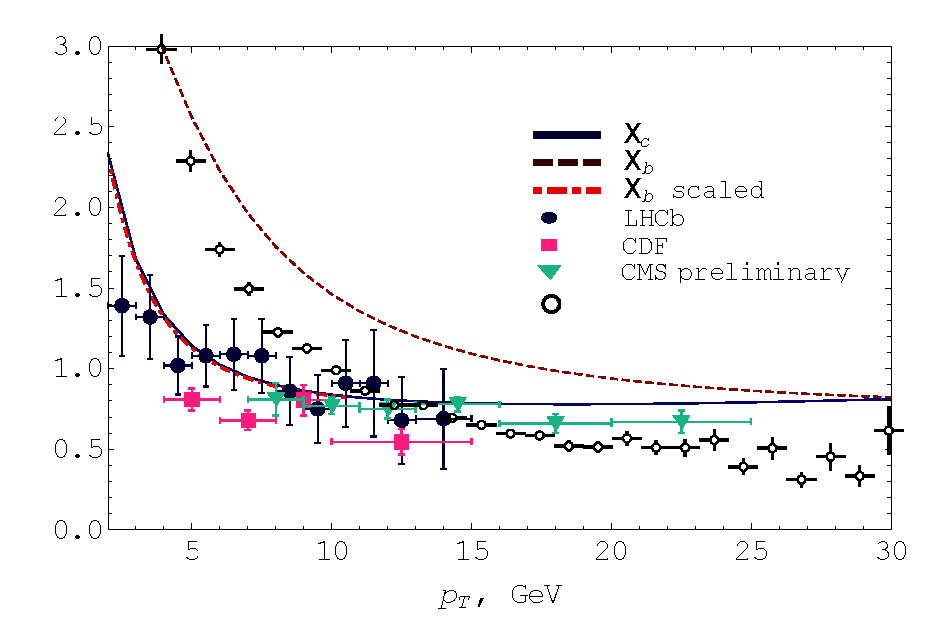
\includegraphics[width=75mm, height=60mm]{ratio/theory}}


     \put(-1,22){\begin{sideways}$\sigma({\chi_2})/\sigma({\chi_1}$)\end{sideways}}
     \put(46,30){\tiny $\chi_b$ scaled}
     \put(45,27){\tiny (this study, MC data)}

    % \graphpaper[5](0,0)(75, 60)
  \end{picture}
  \caption {\small This figure is taken from~\cite{Likhoded:2012hw} and shows
  transverse momentum distributions of the
$d\sigma\left[\chi_{2}\right]/d\sigma[\chi_{1}]$ ratio. Solid and dashed lines
stand for charmonium and bottomonium mesons. The dot-dashed line corresponds to
the rescaled bottomonium ratio:
$\sigma_{b2}/\sigma_{b1}(M_{\chi_c}/M_{\chi)b}\,p_T)$. The experimental results
for charmonium from LHC \cite{LHCb:2012ac} are shown with dots,
CDF~\cite{CDF:2007bra} --- with rectangles, and CMS~
\cite{CMS-PAS-BPH-11-010} --- with triangles. The scaled transverse momentum
distribution of \chib on Monte-Carlo data from this study is shown with open
circles. As it is seen, it almost matches the bottomonium curve. Thus the
results of this work have a reason to be used for fixing the fractions of
\chibone and \chibtwo yields on data. }
  \label{fig:frac:ratio}
\end{figure}

The \chibone and \chibtwo ratio is measured by the following formula in
specified transverse momentum intervals of \Y1S:
\begin{equation}
    \frac{N_{\chibtwo}^{data}}{N_{\chibone}^{data}} = \frac{\sigma(\chibtwo)}{\sigma(\chibone)}
    \frac{Br(\chibtwo\to\Upsilon\gamma)}{Br(\chibone\to\Upsilon\gamma)}\frac{\eps_{\chibtwo}}{\eps_{\chibone}}
\label{eqn:mc_ratio}
\end{equation}
, where $\sigma(\chibtwo) / \sigma(\chibone)$ is a ratio
from~\cite{Likhoded:2012hw}.

\begin{table}[H]
\caption{Branching ratios}
\centering
\begin{tabular}{l}
$Br_1[1P, 1S] = 35\% \pm 8\%$ \\
$Br_2[1P, 1S] = 22\% \pm 4\%$ \\
$Br_1[2P, 1S] = 8.5\% \pm 1.3\%$ \\
$Br_2[2P, 1S] = 7.1\% \pm 1\%$ \\
$Br_1[2P, 2S] = 21\% \pm 4\%$ \\
$Br_2[2P, 2S] = 16\% \pm 2.4\%$ \\
\end{tabular}
\label{tab:branching}
\end{table}


\begin{table}[H]
\caption{Summary of \chibone yield fraction ($\lambda_{\chi_{b1}(1,2P)}$)
determination  in data fits.}
\scalebox{0.6}{
	\begin{tabular}{lcccccccc}
	& \multicolumn8{c}{\OneS transverse momentum interval, \gevc} \\
	 & 6 --- 8 & 8 --- 10 & 10 --- 12 & 12 --- 14 & 14 --- 18 & 18 --- 22 & 22 --- 30 & 18 --- 30 \\
	\hline
	$\frac{\sigma{\chibtwo}}{\sigma{\chibone}}$  & 1.77 $\pm$ 0.17 & 1.50 $\pm$ 0.10 & 1.30 $\pm$ 0.10 & 1.15 $\pm$ 0.05 & 1.05 $\pm$ 0.05 & 0.95 $\pm$ 0.05 & 0.85 $\pm$ 0.05 & 0.90 $\pm$ 0.10 \\

	$\frac{\eps_{\chibtwo(1P)}}{\eps_{\chibone(1P)}}$  & 0.991 $\pm$ 0.013 & 1.029 $\pm$ 0.017 & 0.931 $\pm$ 0.019 & 0.970 $\pm$ 0.025 & 0.963 $\pm$ 0.028 & 1.03 $\pm$ 0.04 & 0.96 $\pm$ 0.05 & 1.003 $\pm$ 0.034 \\
	$\frac{\eps_{\chibtwo(2P)}}{\eps_{\chibone(2P)}}$  & 0.885 $\pm$ 0.015 & 0.873 $\pm$ 0.017 & 0.952 $\pm$ 0.021 & 0.978 $\pm$ 0.026 & 0.961 $\pm$ 0.032 & 1.00 $\pm$ 0.06 & 0.83 $\pm$ 0.07 & 0.95 $\pm$ 0.05 \\


	\rule{0pt}{4ex}$\frac{N_{\chibtwo(1P) \rightarrow \Y1S \gamma}}{N_{\chibone(1P) \rightarrow \Y1S \gamma}}$  & 1.11 $\pm$ 0.34 & 0.97 $\pm$ 0.29 & 0.76 $\pm$ 0.23 & 0.70 $\pm$ 0.21 & 0.64 $\pm$ 0.19 & 0.61 $\pm$ 0.18 & 0.51 $\pm$ 0.16 & 0.57 $\pm$ 0.18 \\

	$\frac{N_{\chibtwo(2P) \rightarrow \Y1S \gamma}}{N_{\chibone(2P) \rightarrow \Y1S \gamma}}$  & 1.31 $\pm$ 0.30 & 1.09 $\pm$ 0.24 & 1.03 $\pm$ 0.23 & 0.94 $\pm$ 0.20 & 0.84 $\pm$ 0.18 & 0.80 $\pm$ 0.18 & 0.59 $\pm$ 0.14 & 0.71 $\pm$ 0.17 \\

	\rule{0pt}{4ex}$\alpha_{\chiboneOneP}$  & 0.47 $\pm$ 0.08 & 0.51 $\pm$ 0.07 & 0.57 $\pm$ 0.07 & 0.59 $\pm$ 0.07 & 0.61 $\pm$ 0.07 & 0.62 $\pm$ 0.07 & 0.66 $\pm$ 0.07 & 0.64 $\pm$ 0.07 \\
	$\alpha_{\chiboneTwoP}$  & 0.43 $\pm$ 0.06 & 0.48 $\pm$ 0.05 & 0.49 $\pm$ 0.06 & 0.52 $\pm$ 0.05 & 0.54 $\pm$ 0.05 & 0.56 $\pm$ 0.06 & 0.63 $\pm$ 0.05 & 0.58 $\pm$ 0.06 \\
	\end{tabular}
}
\label{tab:ratio:lambda}
\end{table}


\section{Simulation}
\label{sec:mc}

% =============================================================================
\subsection{Data - simulation comparison}
\label{sec:mc:datavsmc}

A comparison of the distribution of the relevant observables used in this
analysis was performed on real and simulated data, in order to assess the
reliability of Monte Carlo in computing efficiencies. It should be stressed
that, since a relative branching fraction is measured, systematic effects cancel
at first order.

Combinatorial background has been subtracted in real data by using an
\sPlot  technique~\cite{Pivk:2004ty}.
The resulting signal weights are used to obtain the signal distribution for each
relevant variable. 

% These distributions are compared with simulation, as
% shown in Figures~[\ref{fig:mc:datavsmc:compare1}, \ref{fig:mc:datavsmc:compare2}].

In Figures~\ref{fig:mc:datavsmc:compare1} and \ref{fig:mc:datavsmc:compare2}
these distributions  are shown for signals in $\chib \to \Y1S \gamma$ decays
compared with the corresponding simulated distributions.

The agreement is generally very good except the distribution of photon
transverse momentum ~\ref{fig:mc:datavsmc:gamma}. Imperfect  distribution of
photon transverse momentum can be explained by incorrect sPlot behavior in case
when this technique is applied on variables that affect the background form. In
our study background form depends on the photon transverse momentum.

\begin{figure}[H]
  \setlength{\unitlength}{1mm}
  \centering
  \begin{picture}(150,140)
    %
    \put(0,0){
      \includegraphics*[width=50mm, height=35mm]{mc/vsdata/cl_g_1p}
    }
    \put(50,0){
      \includegraphics*[width=50mm, height=35mm]{mc/vsdata/cl_g_2p}
    }
    \put(100,0){
      \includegraphics*[width=50mm, height=35mm]{mc/vsdata/cl_g_3p}
    }

    \put(0,35){
      \includegraphics*[width=50mm, height=35mm]{mc/vsdata/c2_dtf_1p}
    }
    \put(50,35){
      \includegraphics*[width=50mm, height=35mm]{mc/vsdata/c2_dtf_2p}
    }
    \put(100,35){
      \includegraphics*[width=50mm, height=35mm]{mc/vsdata/c2_dtf_3p}
    }
    \put(0,70){
      \includegraphics*[width=50mm, height=35mm]{mc/vsdata/pt_chib_1p}
    }
    \put(50,70){
      \includegraphics*[width=50mm, height=35mm]{mc/vsdata/pt_chib_2p}
    }
    \put(100,70){
      \includegraphics*[width=50mm, height=35mm]{mc/vsdata/pt_chib_3p}
    }
    \put(0,105){
      \includegraphics*[width=50mm, height=35mm]{mc/vsdata/pt_ups_1p}
    }
    \put(50,105){
      \includegraphics*[width=50mm, height=35mm]{mc/vsdata/pt_ups_2p}
    }
    \put(100,105){
      \includegraphics*[width=50mm, height=35mm]{mc/vsdata/pt_ups_3p}
    }

    \put(15,-1){\scriptsize $\gamma$ confidence level}
    \put(65,-1){\scriptsize $\gamma$ confidence level}
    \put(115,-1){\scriptsize $\gamma$ confidence level}
    \put(10,34){\scriptsize $\chisq$ of decay tree fitter}
    \put(60,34){\scriptsize $\chisq$ of decay tree fitter}
    \put(110,34){\scriptsize $\chisq$ of decay tree fitter}
    \put(20,69){\scriptsize $p_T[\chibOneP] \left[\gevcc\right]$}
    \put(70,69){\scriptsize $p_T[\chibTwoP] \left[\gevcc\right]$}
    \put(120,69){\scriptsize $p_T[\chibThreeP] \left[\gevcc\right]$}
    \put(20,104){\scriptsize $p_T[\Y1S] \left[\gevcc\right]$}
    \put(70,104){\scriptsize $p_T[\Y1S] \left[\gevcc\right]$}
    \put(120,104){\scriptsize $p_T[\Y1S] \left[\gevcc\right]$}

    \put(0,7){\scriptsize \begin{sideways}Arbitrary units\end{sideways}}
    \put(50,7){\scriptsize \begin{sideways}Arbitrary units\end{sideways}}
    \put(100,7){\scriptsize \begin{sideways}Arbitrary units\end{sideways}}
    \put(0,42){\scriptsize \begin{sideways}Arbitrary units\end{sideways}}
    \put(50,42){\scriptsize \begin{sideways}Arbitrary units\end{sideways}}
    \put(100,42){\scriptsize \begin{sideways}Arbitrary units\end{sideways}}
    \put(0,77){\scriptsize \begin{sideways}Arbitrary units\end{sideways}}
    \put(50,77){\scriptsize \begin{sideways}Arbitrary units\end{sideways}}
    \put(100,77){\scriptsize \begin{sideways}Arbitrary units\end{sideways}}
    \put(0,112){\scriptsize \begin{sideways}Arbitrary units\end{sideways}}
    \put(50,112){\scriptsize \begin{sideways}Arbitrary units\end{sideways}}
    \put(100,112){\scriptsize \begin{sideways}Arbitrary units\end{sideways}}

    \put(35,27){\scriptsize \chibOneP}
    \put(85,27){\scriptsize \chibTwoP}
    \put(135,27){\scriptsize \chibThreeP}
    \put(35,62){\scriptsize \chibOneP}
    \put(85,62){\scriptsize \chibTwoP}
    \put(135,62){\scriptsize \chibThreeP}
    \put(35,97){\scriptsize \chibOneP}
    \put(85,97){\scriptsize \chibTwoP}
    \put(135,97){\scriptsize \chibThreeP}
    \put(35,132){\scriptsize \chibOneP}
    \put(85,132){\scriptsize \chibTwoP}
    \put(135,132){\scriptsize \chibThreeP}
 
    % \graphpaper[5](0,0)(150, 175)        
  \end{picture}
  \caption {\small 
    Data (\sqs = 8\tev) --- Monte Carlo values comparison. Square (blue) points
    with errors bars corresponds data values, open circle (red) points with
    errors bars corresponds to simulation values. }
  \label{fig:mc:datavsmc:compare1}
\end{figure}


\begin{figure}[H]
  \setlength{\unitlength}{1mm}
  \centering
  \begin{picture}(150,175)
    %
    \put(0,0){
      \includegraphics*[width=50mm, height=35mm]{mc/vsdata/y_1p}
    }
    \put(50,0){
      \includegraphics*[width=50mm, height=35mm]{mc/vsdata/y_2p}
    }
    \put(100,0){
      \includegraphics*[width=50mm, height=35mm]{mc/vsdata/y_3p}
    }

    \put(0,35){
      \includegraphics*[width=50mm, height=35mm]{mc/vsdata/min_p_mu1_p_mu2_1p}
    }
    \put(50,35){
      \includegraphics*[width=50mm, height=35mm]{mc/vsdata/min_p_mu1_p_mu2_2p}
    }
    \put(100,35){
      \includegraphics*[width=50mm, height=35mm]{mc/vsdata/min_p_mu1_p_mu2_3p}
    }
    \put(0,70){
      \includegraphics*[width=50mm, height=35mm]{mc/vsdata/min_pt_mu1_pt_mu2_1p}
    }
    \put(50,70){
      \includegraphics*[width=50mm, height=35mm]{mc/vsdata/min_pt_mu1_pt_mu2_2p}
    }
    \put(100,70){
      \includegraphics*[width=50mm, height=35mm]{mc/vsdata/min_pt_mu1_pt_mu2_3p}
    }
    \put(0,105){
      \includegraphics*[width=50mm, height=35mm]{mc/vsdata/dll_min_1p}
    }
    \put(50,105){
      \includegraphics*[width=50mm, height=35mm]{mc/vsdata/dll_min_2p}
    }
    \put(100,105){
      \includegraphics*[width=50mm, height=35mm]{mc/vsdata/dll_min_3p}
    }
    \put(0,140){
      \includegraphics*[width=50mm, height=35mm]{mc/vsdata/chi2_vx_1p}
    }
    \put(50,140){
      \includegraphics*[width=50mm, height=35mm]{mc/vsdata/chi2_vx_2p}
    }
    \put(100,140){
      \includegraphics*[width=50mm, height=35mm]{mc/vsdata/chi2_vx_3p}
    }    

    \put(20,-1){\scriptsize \Y1S rapidity}
    \put(70,-1){\scriptsize \Y1S rapidity}
    \put(120,-1){\scriptsize \Y1S rapidity}
    \put(10,34){\scriptsize $min[p(\mu^+), p(\mu^-)] [\gevc]$ }
    \put(60,34){\scriptsize $min[p(\mu^+), p(\mu^-)] [\gevc]$}
    \put(110,34){\scriptsize $min[p(\mu^+), p(\mu^-)] [\gevc]$}
    \put(10,69){\scriptsize $min[p_T(\mu^+), p_T(\mu^-)] [\gevc]$}
    \put(60,69){\scriptsize $min[p_T(\mu^+), p_T(\mu^-)] [\gevc]$}
    \put(110,69){\scriptsize $min[p_T(\mu^+), p_T(\mu^-)] [\gevc]$}
    \put(20,104){\scriptsize $\Delta\log\lum^{\mmu-\Ph}$}
    \put(70,104){\scriptsize $\Delta\log\lum^{\mmu-\Ph}$}
    \put(120,104){\scriptsize $\Delta\log\lum^{\mmu-\Ph}$}
    \put(10,139){\scriptsize $\chisq$ for decay vertex fitter}
    \put(60,139){\scriptsize $\chisq$ for decay vertex fitter}
    \put(110,139){\scriptsize $\chisq$ for decay vertex fitter}

    \put(0,7){\scriptsize \begin{sideways}Arbitrary units\end{sideways}}
    \put(50,7){\scriptsize \begin{sideways}Arbitrary units\end{sideways}}
    \put(100,7){\scriptsize \begin{sideways}Arbitrary units\end{sideways}}
    \put(0,42){\scriptsize \begin{sideways}Arbitrary units\end{sideways}}
    \put(50,42){\scriptsize \begin{sideways}Arbitrary units\end{sideways}}
    \put(100,42){\scriptsize \begin{sideways}Arbitrary units\end{sideways}}
    \put(0,77){\scriptsize \begin{sideways}Arbitrary units\end{sideways}}
    \put(50,77){\scriptsize \begin{sideways}Arbitrary units\end{sideways}}
    \put(100,77){\scriptsize \begin{sideways}Arbitrary units\end{sideways}}
    \put(0,112){\scriptsize \begin{sideways}Arbitrary units\end{sideways}}
    \put(50,112){\scriptsize \begin{sideways}Arbitrary units\end{sideways}}
    \put(100,112){\scriptsize \begin{sideways}Arbitrary units\end{sideways}}
    \put(0,147){\scriptsize \begin{sideways}Arbitrary units\end{sideways}}
    \put(50,147){\scriptsize \begin{sideways}Arbitrary units\end{sideways}}
    \put(100,147){\scriptsize \begin{sideways}Arbitrary units\end{sideways}}

    \put(35,27){\scriptsize \chibOneP}
    \put(85,27){\scriptsize \chibTwoP}
    \put(135,27){\scriptsize \chibThreeP}
    \put(35,62){\scriptsize \chibOneP}
    \put(85,62){\scriptsize \chibTwoP}
    \put(135,62){\scriptsize \chibThreeP}
    \put(35,97){\scriptsize \chibOneP}
    \put(85,97){\scriptsize \chibTwoP}
    \put(135,97){\scriptsize \chibThreeP}
    \put(35,132){\scriptsize \chibOneP}
    \put(85,132){\scriptsize \chibTwoP}
    \put(135,132){\scriptsize \chibThreeP}
    \put(35,167){\scriptsize \chibOneP}
    \put(85,167){\scriptsize \chibTwoP}
    \put(135,167){\scriptsize \chibThreeP}
 
    % \graphpaper[5](0,0)(150, 175)        
  \end{picture}
  \caption {\small 
    Data (\sqs = 8\tev) --- Monte Carlo values comparison. Square (blue) points
    with errors bars corresponds data values, open circle (red) points with
    errors bars corresponds to simulation values. }
  \label{fig:mc:datavsmc:compare2}
\end{figure}

\begin{figure}[H]
  \setlength{\unitlength}{1mm}
  \centering
  \begin{picture}(150,35)
    %
    \put(0,0){
      \includegraphics*[width=50mm, height=35mm]{mc/vsdata/pt_g_1p}
    }
    \put(50,0){
      \includegraphics*[width=50mm, height=35mm]{mc/vsdata/pt_g_2p}
    }
    \put(100,0){
      \includegraphics*[width=50mm, height=35mm]{mc/vsdata/pt_g_3p}
    }

    \put(20,-1){\scriptsize $p_T(\gamma)$ $\left[\gevc\right]$}
    \put(70,-1){\scriptsize $p_T(\gamma)$ $\left[\gevc\right]$}
    \put(120,-1){\scriptsize $p_T(\gamma)$ $\left[\gevc\right]$}


    \put(0,7){\scriptsize \begin{sideways}Arbitrary units\end{sideways}}
    \put(50,7){\scriptsize \begin{sideways}Arbitrary units\end{sideways}}
    \put(100,7){\scriptsize \begin{sideways}Arbitrary units\end{sideways}}

    \put(35,27){\scriptsize \chibOneP}
    \put(85,27){\scriptsize \chibTwoP}
    \put(135,27){\scriptsize \chibThreeP}
 
    % \graphpaper[5](0,0)(150, 175)        
  \end{picture}
  \caption {\small 
    Data (\sqs = 8\tev) - Monte Carlo values comparison. Square (blue) points
    with errors bars corresponds data values, open circle (red) points with
    errors bars corresponds to simulation values. }
  \label{fig:mc:datavsmc:gamma}
\end{figure}

% =============================================================================
\subsection{Selection efficiencies}
\label{sec:mc:eff}

The invariant mass difference distributions of matched events in the \chib
simulation are shown in Figure~\ref{fig:mc:eff:nominal}. The left tails are
almost flat at these plots, so on the real data the signal events in these parts
are hard to separate from background. For this reason the number of MC-true
\chib events for efficiency measurements were obtained by performing a fit with
the background component that matches events the tails. The number of $\Upsilon$
events is obtained by counting MC-true $\Upsilon$ events.

\begin{figure}[H]
  \setlength{\unitlength}{1mm}
  \centering
  \scalebox{0.5}{
  \begin{picture}(225,120)
    \put(0,60){
      \includegraphics*[width=75mm, height=60mm]{mc/eff/cb11_6_40}
    }
    \put(42,114){\scriptsize $\chiboneOneP \to \Y1S \gamma$}
    \put(42,109){\scriptsize $6 < p_T^{\Y1S} < 40 \gevc$}
    \put(10,73){$m_{\mumu \gamma} - m_{\mumu} + 9.4603 \left[\gevcc\right]$}
    \put(3,85){\scriptsize \begin{sideways}Candidates/(10\mevcc)\end{sideways}}    
    \put(45,103){\scriptsize N =34,330 $\pm$ 220}
    \put(45,100){\scriptsize B/N = 15.3 $\pm$ 0.4\%}
    

    \put(75,60){
      \includegraphics*[width=75mm, height=60mm]{mc/eff/cb12_6_40}
    }
    \put(117,114){\scriptsize $\chiboneTwoP \to \Y1S \gamma$}
    \put(117,109){\scriptsize $6 < p_T^{\Y1S} < 40 \gevc$}
    \put(85,73){$m_{\mumu \gamma} - m_{\mumu} + 9.4603 \left[\gevcc\right]$}
    \put(78,85){\scriptsize \begin{sideways}Candidates/(10\mevcc)\end{sideways}}    
    \put(120,103){\scriptsize N =22,210 $\pm$ 170}
    \put(120,100){\scriptsize B/N = 10.3 $\pm$ 0.4\%}
    

    \put(150,60){
      \includegraphics*[width=75mm, height=60mm]{mc/eff/cb13_6_40}
    }
    \put(192,114){\scriptsize $\chiboneThreeP \to \Y1S \gamma$}
    \put(192,109){\scriptsize $6 < p_T^{\Y1S} < 40 \gevc$}
    \put(160,73){$m_{\mumu \gamma} - m_{\mumu} + 9.4603 \left[\gevcc\right]$}
    \put(153,85){\scriptsize \begin{sideways}Candidates/(10\mevcc)\end{sideways}}    
    \put(195,103){\scriptsize N =15,110 $\pm$ 130}
    \put(195,100){\scriptsize B/N = 9.0 $\pm$ 0.4\%}
    

    \put(0,0){
      \includegraphics*[width=75mm, height=60mm]{mc/eff/cb12_18_40}
    }
    \put(42,54){\scriptsize $\chiboneTwoP \to \Y2S \gamma$}
    \put(42,49){\scriptsize $18 < p_T^{\Y1S} < 40 \gevc$}
    \put(10,13){$m_{\mumu \gamma} - m_{\mumu} + 10.02326 \left[\gevcc\right]$}
    \put(3,25){\scriptsize \begin{sideways}Candidates/(10\mevcc)\end{sideways}}    
    \put(45,43){\scriptsize N =194 $\pm$ 21}
    \put(45,40){\scriptsize B/N = 8 $\pm$ 9\%}
    

    \put(75,0){
      \includegraphics*[width=75mm, height=60mm]{mc/eff/cb13_18_40}
    }
    \put(117,54){\scriptsize $\chiboneThreeP \to \Y2S \gamma$}
    \put(117,49){\scriptsize $18 < p_T^{\Y1S} < 40 \gevc$}
    \put(85,13){$m_{\mumu \gamma} - m_{\mumu} + 10.02326 \left[\gevcc\right]$}
    \put(78,25){\scriptsize \begin{sideways}Candidates/(10\mevcc)\end{sideways}}    
    \put(120,43){\scriptsize N =672 $\pm$ 32}
    \put(120,40){\scriptsize B/N = 8.5 $\pm$ 3.1\%}
    

    \put(150,0){
      \includegraphics*[width=75mm, height=60mm]{mc/eff/cb13_27_40}
    }
    \put(192,54){\scriptsize $\chiboneThreeP \to \Y3S \gamma$}
    \put(192,49){\scriptsize $27 < p_T^{\Y1S} < 40 \gevc$}
    \put(160,13){$m_{\mumu \gamma} - m_{\mumu} + 10.355 \left[\gevcc\right]$}
    \put(153,25){\scriptsize \begin{sideways}Candidates/(10\mevcc)\end{sideways}}    
    \put(195,43){\scriptsize N =154 $\pm$ 17}
    \put(195,40){\scriptsize B/N = 73 $\pm$ 13\%}
    

     % \graphpaper[5](0,0)(225, 120)        
  \end{picture}
  }
  \caption {\small 
    Distribution of the mass difference $\mumu \gamma - \mumu$ for matched
    $\chi_{b1}(1,2,3P)$ candidates in $\chib \to \Upsilon \gamma$ decays (black
    points) together with the result of the fit (solid red curve), including
    background (dotted blue curve) contribution.The pull is defined as the
    difference  between the data and fit value divided by the data error. }
  \label{fig:mc:eff:nominal}
\end{figure}

Figure~\ref{fig:mc:eff} show the measured efficiency of \chib reconstruction.
More details on these measurements are show in
Tables~[\ref{tab:mc:eff:chib1_y1}--\ref{tab:mc:eff:chib3_y3}] in Appendix.


\begin{figure}[H]
  \setlength{\unitlength}{1mm}
  \centering
  \scalebox{ 0.7 }{
  \begin{picture}(225,60)
    
    %% =======================================================================
    \put(0,0){
      \includegraphics*[width=75mm, height=60mm]{mc/eff/cb_ups1s}
    }
    \put(2,25){\begin{sideways}Efficiency\end{sideways}}
    \put(35,2){$p_T^{\Y1S} \left[\gevc\right]$}
    \put(50,25){\textcolor{blue}{\chibOneP}}
    \put(50,20){\textcolor{red}{\chibTwoP}}
    \put(50,15){\textcolor{cyan}{\chibThreeP}}
    
    \put(45,25){\includegraphics*[width=3mm, height=2mm]{bsf}}
    \put(45,20){\includegraphics*[width=3mm, height=2mm]{rco}}
    \put(45,15){\includegraphics*[width=3mm, height=2mm]{ctuc}}

    \put(45,30){$\chib \to \Y1S \gamma$}
    
    %% =======================================================================
    \put(75,0){
      \includegraphics*[width=75mm, height=60mm]{mc/eff/cb_ups2s}
    }
    \put(77,25){\begin{sideways}Efficiency\end{sideways}}
    \put(110,2){$p_T^{\Y2S} \left[\gevc\right]$}
    
    \put(125,20){\textcolor{red}{\chibTwoP}}
    \put(125,15){\textcolor{cyan}{\chibThreeP}}
    
    
    \put(120,20){\includegraphics*[width=3mm, height=2mm]{rco}}
    \put(120,15){\includegraphics*[width=3mm, height=2mm]{ctuc}}

    \put(120,30){$\chib \to \Y2S \gamma$}
    
    %% =======================================================================
    \put(150,0){
      \includegraphics*[width=75mm, height=60mm]{mc/eff/cb_ups3s}
    }
    \put(152,25){\begin{sideways}Efficiency\end{sideways}}
    \put(185,2){$p_T^{\Y3S} \left[\gevc\right]$}
    
    
    \put(200,15){\textcolor{cyan}{\chibThreeP}}
    
    
    
    \put(195,15){\includegraphics*[width=3mm, height=2mm]{ctuc}}

    \put(195,30){$\chib \to \Y3S \gamma$}
  % \graphpaper[5](0,0)(75, 60)
  \end{picture}
  }
  \caption {\small
    The \chib reconstruction efficiency as function of $p_T^{\Upsilon}$
  }
  \label{fig:mc:eff}
\end{figure}

\section{The \texorpdfstring{$\Upsilon$}{Y} fractions in \texorpdfstring{$\chib \to \Upsilon \gamma$}{chib --> Y gamma} decays}
\label{sec:mc}

Figure~\ref{fig:frac} shows the measured fractions of $\Upsilon$ originating
from \chib decays for different $p_T^{\Upsilon}$ bins,  assuming production of
unpolarized $\Upsilon$ and \chib mesons. The obtained \Y1S fraction is
consistent with the previous LHCb result~\cite{LHCb-PAPER-2012-015}.

\begin{figure}[H]
  \setlength{\unitlength}{1mm}
  \centering
  \resizebox{\textwidth}{!}{
  \begin{picture}(150,120)
    %% =======================================================================
    \put(0,60){
      \includegraphics*[width=75mm, height=60mm]{frac/ups1s}
    }
    \put(2,85){\begin{sideways}\Y1S fraction, \% \end{sideways}}
    \put(35,62){$p_T^{\Y1S} \left[\gevc\right]$}

    % \put(15,113){\scriptsize $\chi_b(1,2,3P) \to \Y1S \gamma$}
    
    \put(55,113){\scriptsize \textcolor{blue}{\sqs=7\tev}}
    \put(55,109){\scriptsize \textcolor{red}{\sqs=8\tev}}
    % \put(48,140){\scriptsize \textcolor{cyan}{\sqs=7\tev (2010)}}
    
    \put(15,113){\includegraphics*[width=2mm, height=2mm]{markers/circle-blue-open}}
    \put(17,113){\includegraphics*[width=2mm, height=2mm]{markers/circle-red-filled}}
    \put(20,114){\tiny $\chibOneP \to \Y1S \gamma$}

    \put(15,110){\includegraphics*[width=2mm, height=2mm]{markers/tri-blue-open}}
    \put(17,110){\includegraphics*[width=2mm, height=2mm]{markers/tri-red-filled}}
    \put(20,111){\tiny $\chibTwoP \to \Y1S \gamma$}

    \put(15,107){\includegraphics*[width=2mm, height=2mm]{markers/sq-blue-open}}
    \put(17,107){\includegraphics*[width=2mm, height=2mm]{markers/sq-red-filled}}
    \put(20,108){\tiny $\chibThreeP \to \Y1S \gamma$}    

    %% =======================================================================
    \put(75,60){
      \includegraphics*[width=75mm, height=60mm]{frac/ups2s}
    }
    \put(77,85){\begin{sideways}\Y2S fraction, \% \end{sideways}}
    \put(110,62){$p_T^{\Y2S} \left[\gevc\right]$}

    % \put(90,113){\scriptsize $\chi_b(2,3P) \to \Y2S \gamma$}
    
    \put(130,113){\scriptsize \textcolor{blue}{\sqs=7\tev}}
    \put(130,109){\scriptsize \textcolor{red}{\sqs=8\tev}}
    
    
    \put(90,113){\includegraphics*[width=2mm, height=2mm]{markers/tri-blue-open}}
    \put(92,113){\includegraphics*[width=2mm, height=2mm]{markers/tri-red-filled}}
    \put(95,114){\tiny $\chibTwoP \to \Y2S \gamma$}

    \put(90,110){\includegraphics*[width=2mm, height=2mm]{markers/sq-blue-open}}
    \put(92,110){\includegraphics*[width=2mm, height=2mm]{markers/sq-red-filled}}
    \put(95,111){\tiny $\chibThreeP \to \Y2S \gamma$}    

    
    %% =======================================================================
    \put(0,0){
      \includegraphics*[width=75mm, height=60mm]{frac/ups3s}
    }
    \put(2,25){\begin{sideways}\Y3S fraction, \% \end{sideways}}
    \put(35,2){$p_T^{\Y3S} \left[\gevc\right]$}

    % \put(15,53){\scriptsize $\chi_b(3P) \to \Y3S \gamma$}
    
    \put(55,52){\scriptsize \textcolor{blue}{\sqs=7\tev}}
    \put(55,48){\scriptsize \textcolor{red}{\sqs=8\tev}}
    
    \put(15,53){\includegraphics*[width=2mm, height=2mm]{markers/sq-blue-open}}
    \put(17,53){\includegraphics*[width=2mm, height=2mm]{markers/sq-red-filled}}
    \put(20,54){\tiny $\chibThreeP \to \Y3S \gamma$}    

   
  % \graphpaper[5](0,0)(150, 120)
  \end{picture}
  }
  \caption{\small
    Fracton of $\Upsilon$ mesons originated from \chib decays (statistical
    errors only}
  \label{fig:frac}
\end{figure}



Tables~[\ref{tab:frac:ups1s}, \ref{tab:frac:ups2s}] provide the summary
of obtained yields, efficiency and fractions.

\begin{table}[H]
\centering
\caption{\small Summary of \Y1S fraction determination originating from \chib decay}
\subtable[$6 < p_T^{\Y1S} < 14 \gevc$] {
\scalebox{0.6}{

\begin{tabular}{lrrrrrr}\toprule
 & \multicolumn{6}{c}{$\Upsilon(1S)$ transverse momentum intervals, \gevc}\\
 & \multicolumn{2}{c}{6 -- 8} & \multicolumn{2}{c}{8 -- 10} & \multicolumn{2}{c}{10 -- 14}\\
\cmidrule(r){2-3}\cmidrule(r){4-5}\cmidrule(r){6-7}
 & \multicolumn{1}{c}{\sqs = 7\tev} & \multicolumn{1}{c}{\sqs = 8\tev} & \multicolumn{1}{c}{\sqs = 7\tev} & \multicolumn{1}{c}{\sqs = 8\tev} & \multicolumn{1}{c}{\sqs = 7\tev} & \multicolumn{1}{c}{\sqs = 8\tev}\\
\midrule
$N_{\chi_b(1P)}$ & 3030 $\pm$ 220 & 6800 $\pm$ 400 & 2410 $\pm$ 130 & 5690 $\pm$ 210 & 2990 $\pm$ 110 & 7340 $\pm$ 180\\
$N_{\chi_b(2P)}$ & 860 $\pm$ 170 & 1490 $\pm$ 290 & 910 $\pm$ 100 & 1790 $\pm$ 170 & 640 $\pm$ 80 & 1020 $\pm$ 130\\
$N_{\chi_b(3P)}$ & --- & --- & --- & --- & 260 $\pm$ 80 & 450 $\pm$ 130\\

\rule{0pt}{4ex}$N_{\Upsilon(1S)}$ & 124,100 $\pm$ 400 & 282,600 $\pm$ 600 & 70,480 $\pm$ 290 & 164,300 $\pm$ 500 & 60,780 $\pm$ 270 & 143,700 $\pm$ 400\\

\rule{0pt}{4ex}$\eps_{\chi_b(1P) \to \Upsilon(1S) \gamma}^{\gamma}$, \% & 12.60 $\pm$ 0.07 & 12.57 $\pm$ 0.07 & 16.06 $\pm$ 0.11 & 15.75 $\pm$ 0.10 & 19.51 $\pm$ 0.13 & 18.92 $\pm$ 0.13\\
$\eps_{\chi_b(2P) \to \Upsilon(1S) \gamma}^{\gamma}$, \% & 19.54 $\pm$ 0.09 & 19.08 $\pm$ 0.10 & 20.69 $\pm$ 0.12 & 20.29 $\pm$ 0.13 & 22.13 $\pm$ 0.14 & 21.40 $\pm$ 0.16\\
$\eps_{\chi_b(3P) \to \Upsilon(1S) \gamma}^{\gamma}$, \% & --- & --- & --- & --- & 21.18 $\pm$ 0.17 & 21.02 $\pm$ 0.18\\
\midrule
Fraction $\chi_b(1P)$, \% & \textbf{19.4 $\pm$ 1.4} & \textbf{19.1 $\pm$ 1.0} & \textbf{21.3 $\pm$ 1.2} & \textbf{22.0 $\pm$ 0.8} & \textbf{25.2 $\pm$ 1.0} & \textbf{27.0 $\pm$ 0.7}\\
Fraction $\chi_b(2P)$, \% & \textbf{3.5 $\pm$ 0.7} & \textbf{2.8 $\pm$ 0.5} & \textbf{6.3 $\pm$ 0.7} & \textbf{5.4 $\pm$ 0.5} & \textbf{4.8 $\pm$ 0.6} & \textbf{3.3 $\pm$ 0.4}\\
Fraction $\chi_b(3P)$, \% & --- & --- & --- & --- & \textbf{2.0 $\pm$ 0.6} & \textbf{1.5 $\pm$ 0.4}\\
\bottomrule
\end{tabular}
} % scalebox/resizebox

} % subtable
\subtable[$14 < p_T^{\Y1S} < 40 \gevc$] {
\scalebox{0.6}{

\begin{tabular}{lrrrrrr}\toprule
 & \multicolumn{6}{c}{$\Upsilon(1S)$ transverse momentum intervals, \gevc}\\
 & \multicolumn{2}{c}{14 -- 18} & \multicolumn{2}{c}{18 -- 22} & \multicolumn{2}{c}{22 -- 40}\\
\cmidrule(r){2-3}\cmidrule(r){4-5}\cmidrule(r){6-7}
 & \multicolumn{1}{c}{\sqs = 7\tev} & \multicolumn{1}{c}{\sqs = 8\tev} & \multicolumn{1}{c}{\sqs = 7\tev} & \multicolumn{1}{c}{\sqs = 8\tev} & \multicolumn{1}{c}{\sqs = 7\tev} & \multicolumn{1}{c}{\sqs = 8\tev}\\
\midrule
$N_{\chi_b(1P)}$ & 1170 $\pm$ 60 & 2840 $\pm$ 100 & 452 $\pm$ 32 & 1130 $\pm$ 50 & 318 $\pm$ 24 & 740 $\pm$ 40\\
$N_{\chi_b(2P)}$ & 250 $\pm$ 40 & 580 $\pm$ 60 & 85 $\pm$ 16 & 156 $\pm$ 25 & 57 $\pm$ 11 & 167 $\pm$ 19\\
$N_{\chi_b(3P)}$ & 90 $\pm$ 31 & 130 $\pm$ 50 & 25 $\pm$ 10 & 33 $\pm$ 16 & 24 $\pm$ 8 & 42 $\pm$ 11\\

\rule{0pt}{4ex}$N_{\Upsilon(1S)}$ & 18,520 $\pm$ 150 & 45,160 $\pm$ 230 & 5960 $\pm$ 90 & 15,600 $\pm$ 140 & 3690 $\pm$ 70 & 9270 $\pm$ 110\\

\rule{0pt}{4ex}$\eps_{\chi_b(1P) \to \Upsilon(1S) \gamma}^{\gamma}$, \% & 22.70 $\pm$ 0.31 & 22.99 $\pm$ 0.28 & 24.7 $\pm$ 0.6 & 25.2 $\pm$ 0.6 & 26.7 $\pm$ 1.0 & 25.9 $\pm$ 0.9\\
$\eps_{\chi_b(2P) \to \Upsilon(1S) \gamma}^{\gamma}$, \% & 23.26 $\pm$ 0.29 & 23.04 $\pm$ 0.32 & 23.6 $\pm$ 0.6 & 23.0 $\pm$ 0.6 & 23.9 $\pm$ 0.9 & 22.3 $\pm$ 0.9\\
$\eps_{\chi_b(3P) \to \Upsilon(1S) \gamma}^{\gamma}$, \% & 22.4 $\pm$ 0.4 & 21.6 $\pm$ 0.4 & 21.8 $\pm$ 0.7 & 20.8 $\pm$ 0.7 & 21.2 $\pm$ 1.0 & 21.6 $\pm$ 1.0\\
\midrule
Fraction $\chi_b(1P)$, \% & \textbf{27.9 $\pm$ 1.5} & \textbf{27.4 $\pm$ 1.0} & \textbf{30.7 $\pm$ 2.3} & \textbf{28.7 $\pm$ 1.5} & \textbf{32.3 $\pm$ 2.8} & \textbf{30.8 $\pm$ 2.0}\\
Fraction $\chi_b(2P)$, \% & \textbf{5.8 $\pm$ 0.9} & \textbf{5.6 $\pm$ 0.6} & \textbf{6.1 $\pm$ 1.1} & \textbf{4.4 $\pm$ 0.7} & \textbf{6.5 $\pm$ 1.3} & \textbf{8.1 $\pm$ 1.0}\\
Fraction $\chi_b(3P)$, \% & \textbf{2.2 $\pm$ 0.7} & \textbf{1.3 $\pm$ 0.5} & \textbf{1.9 $\pm$ 0.8} & \textbf{1.0 $\pm$ 0.5} & \textbf{3.0 $\pm$ 1.0} & \textbf{2.1 $\pm$ 0.6}\\
\bottomrule
\end{tabular}
} % scalebox/resizebox

} % subtable
\label{tab:frac:ups1s}
\end{table}

\begin{table}[H]
\centering
\caption{\small Summary of \Y2S fraction determination originating from \chib decay}
\subtable[$18 < p_T^{\Y2S} < 24 \gevc$] {
\scalebox{0.5}{

\begin{tabular}{lrrrrrrrr}\toprule
 & \multicolumn{8}{c}{$\Upsilon(2S)$ transverse momentum intervals, \gevc}\\
 & \multicolumn{2}{c}{18 -- 20} & \multicolumn{2}{c}{18 -- 40} & \multicolumn{2}{c}{20 -- 22} & \multicolumn{2}{c}{22 -- 24}\\
\cmidrule(r){2-3}\cmidrule(r){4-5}\cmidrule(r){6-7}\cmidrule(r){8-9}
 & \multicolumn{1}{c}{\sqs = 7\tev} & \multicolumn{1}{c}{\sqs = 8\tev} & \multicolumn{1}{c}{\sqs = 7\tev} & \multicolumn{1}{c}{\sqs = 8\tev} & \multicolumn{1}{c}{\sqs = 7\tev} & \multicolumn{1}{c}{\sqs = 8\tev} & \multicolumn{1}{c}{\sqs = 7\tev} & \multicolumn{1}{c}{\sqs = 8\tev}\\
\midrule
$N_{\chi_b(2P)}$ & 101 $\pm$ 18 & 223 $\pm$ 28 & --- & --- & 65 $\pm$ 15 & 152 $\pm$ 23 & 41 $\pm$ 12 & 94 $\pm$ 18\\
$N_{\chi_b(3P)}$ & --- & --- & 48 $\pm$ 17 & 68 $\pm$ 26 & --- & --- & --- & ---\\

\rule{0pt}{4ex}$N_{\Upsilon(2S)}$ & 1870 $\pm$ 50 & 4420 $\pm$ 80 & 4860 $\pm$ 80 & 11,910 $\pm$ 130 & 1120 $\pm$ 40 & 2790 $\pm$ 60 & 591 $\pm$ 29 & 1480 $\pm$ 50\\

\rule{0pt}{4ex}$\eps_{\chi_b(2P) \to \Upsilon(2S) \gamma}^{\gamma}$, \% & 16.4 $\pm$ 0.7 & 15.9 $\pm$ 0.7 & --- & --- & 18.2 $\pm$ 0.9 & 17.8 $\pm$ 1.0 & 18.5 $\pm$ 1.2 & 20.1 $\pm$ 1.4\\
$\eps_{\chi_b(3P) \to \Upsilon(2S) \gamma}^{\gamma}$, \% & --- & --- & 22.3 $\pm$ 0.6 & 22.3 $\pm$ 0.5 & --- & --- & --- & ---\\
\midrule
Fraction $\chi_b(2P)$, \% & \textbf{33 $\pm$ 6} & \textbf{32 $\pm$ 4} & --- & --- & \textbf{32 $\pm$ 7} & \textbf{31 $\pm$ 5} & \textbf{37 $\pm$ 11} & \textbf{31 $\pm$ 7}\\
Fraction $\chi_b(3P)$, \% & --- & --- & \textbf{4.4 $\pm$ 1.6} & \textbf{2.6 $\pm$ 1.0} & --- & --- & --- & ---\\
\bottomrule
\end{tabular}
} % scalebox/resizebox

} % subtable
\subtable[$24 < p_T^{\Y2S} < 40 \gevc$] {
\scalebox{0.5}{

\begin{tabular}{lrrrr}\toprule
 & \multicolumn{4}{c}{$\Upsilon(2S)$ transverse momentum intervals, \gevc}\\
 & \multicolumn{2}{c}{24 -- 28} & \multicolumn{2}{c}{28 -- 40}\\
\cmidrule(r){2-3}\cmidrule(r){4-5}
 & \multicolumn{1}{c}{\sqs = 7\tev} & \multicolumn{1}{c}{\sqs = 8\tev} & \multicolumn{1}{c}{\sqs = 7\tev} & \multicolumn{1}{c}{\sqs = 8\tev}\\
\midrule
$N_{\chi_b(2P)}$ & 39 $\pm$ 12 & 135 $\pm$ 20 & 35 $\pm$ 9 & 93 $\pm$ 15\\
$N_{\chi_b(3P)}$ & --- & --- & --- & ---\\

\rule{0pt}{4ex}$N_{\Upsilon(2S)}$ & 719 $\pm$ 33 & 1770 $\pm$ 50 & 505 $\pm$ 29 & 1330 $\pm$ 50\\

\rule{0pt}{4ex}$\eps_{\chi_b(2P) \to \Upsilon(2S) \gamma}^{\gamma}$, \% & 19.4 $\pm$ 1.3 & 22.9 $\pm$ 1.4 & 23.6 $\pm$ 1.7 & 23.9 $\pm$ 1.8\\
$\eps_{\chi_b(3P) \to \Upsilon(2S) \gamma}^{\gamma}$, \% & --- & --- & --- & ---\\
\midrule
Fraction $\chi_b(2P)$, \% & \textbf{28 $\pm$ 9} & \textbf{33 $\pm$ 5} & \textbf{29 $\pm$ 8} & \textbf{29 $\pm$ 5}\\
Fraction $\chi_b(3P)$, \% & --- & --- & --- & ---\\
\bottomrule
\end{tabular}
} % scalebox/resizebox

} % subtable
\label{tab:frac:ups2s}
\end{table}

\begin{table}[H]
\caption{\small Summary of \Y3S fraction determination originating from \chib decay}
\centering
\scalebox{1}{

\begin{tabular}{lrrrr}\toprule
 & \multicolumn{4}{c}{$\Upsilon(3S)$ transverse momentum intervals, \gevc}\\
 & \multicolumn{2}{c}{24 -- 29} & \multicolumn{2}{c}{29 -- 40}\\
\cmidrule(r){2-3}\cmidrule(r){4-5}
 & \multicolumn{1}{c}{\sqs = 7\tev} & \multicolumn{1}{c}{\sqs = 8\tev} & \multicolumn{1}{c}{\sqs = 7\tev} & \multicolumn{1}{c}{\sqs = 8\tev}\\
\midrule
$N_{\chi_b(3P)}$ & 32 $\pm$ 8 & 69 $\pm$ 13 & 27 $\pm$ 7 & 86 $\pm$ 12\\

\rule{0pt}{4ex}$N_{\Upsilon(3S)}$ & 521 $\pm$ 30 & 1350 $\pm$ 50 & 274 $\pm$ 23 & 790 $\pm$ 40\\

\rule{0pt}{4ex}$\eps_{\chi_b(3P) \to \Upsilon(3S) \gamma}^{\gamma}$, \% & 15.1 $\pm$ 1.0 & 12.9 $\pm$ 1.0 & 19.8 $\pm$ 2.1 & 22.1 $\pm$ 2.4\\
\midrule
Fraction $\chi_b(3P)$, \% & \textbf{41 $\pm$ 11} & \textbf{40 $\pm$ 8} & \textbf{50 $\pm$ 15} & \textbf{50 $\pm$ 9}\\
\bottomrule
\end{tabular}
} % scalebox/resizebox
\label{tab:frac:ups3s}
\end{table}
\section{Systematic Uncertainties}
\label{sec:syst}

This analysis measures the fraction of $\Upsilon(nS)$ particles originating
from $\chi_b$ decays, most systematic uncertainties cancel in the ratio and
only residual effects need to be taken into account. Systematic uncertainties
can be grouped according to various sources, related respectively to:
\begin{itemize}
\item the fit model of $\Upsilon$ and $\chi_b$ invariant masses, 
\item the determination of the photon reconstruction efficiency, and 
\item the unknown initial polarization of $\chi_b$ and $\Upsilon$ particles. 
\end{itemize}
These uncertainties will be detailed in the following. 

\subsection{Uncertainties related to the fit model}

The uncertainty related to the modeling of the $\Upsilon$ invariant mass
distribution has been estimated by following previous
studies~\ref{Aaij:2013yaa}. An uncertainty of 0.7\% has been assigned to the
yields of $\Upsilon(nS)$ mesons.

In the fit model of the $chi_b$ invariant masses, several sources need to be
taken into account. Firstly, the relative proportion of spin-1 and spin-2
states, which is kept fixed in the fit to values close to 0.5, predicted by
theory, is varied from 0.4 to 0.7. 

Tables [\ref{tab:syst:lambda1s}-\ref{tab:syst:lambda2s}] reports the relative
variation in percent of the $\chi_b$ yields as function of $\lambda$, the
relative proportion of the two $\chi_b$ states, for all examined decays, in
each bin of $\Upsilon(nS)$ transverse momentum. We take as systematic error in
each $p_T$ bin the maximum variation of the $\chi_b$ yields with respect to the
nominal fit.

Another source of systematic is due to the variation of the $\chi_b$ masses as
function of $p_T(\Upsilon)$, observed in Section~\ref{relevant_section_here}.
We repeat the fits by taking the minimum and maximum values of the $\chi_b$
masses and take the maximum difference in the yields as systematic uncertainty.
The resulting uncertainties are reported in
Tables~\ref{tab:syst:m1p}-\ref{tab:syst:m3p}.


Other uncertainties due to parameters taken from PDG (e.g. mass differences)
are assumed to be negligible.

\subsubsection{Uncertainties related to the data-MonteCarlo resolution difference}

In the $\chi_b$ fits, the resolution of the Crystal Ball functions, determined
from simulation, has been scaled by a factor 1.16 in order to account for data ---
MonteCarlo differences. This factor was obtained by fitting a histogram, 
that store the ratio between data and MonteCarlo resolution, by constant function.
The result of fit is shown in Figure~\ref{fig:syst:ratio_data_mc_sigma}.

We estimate the systematic uncertainty due to this assumption by repeating the
fits without scaling the $\sigma$ parameter of the CB functions. Results are
shown in Table~\ref{relevant_tables_here}.

\begin{figure}[H]
  \setlength{\unitlength}{1mm}
  \centering
  \begin{picture}(75, 60)
  \put(0,0){
    \includegraphics*[width=75mm, height=60mm]{syst/sigma_b1_1p}
  }
  \put(50,0){$p_T^{\Y1S} \left[\gevc\right]$}
  \put(0,20){\begin{sideways} $\sigma_{\chiboneOneP} \left[\gevcc\right]$ \end{sideways}}
  
  \put(45,50){\includegraphics*[width=4mm, height=2mm]{blue}}
  \put(45,45){\includegraphics*[width=4mm, height=2mm]{red}}
  \put(49,50){\sqs=7\tev}
  \put(49,45){\sqs=8\tev}



  \end{picture}
  \label{fig:syst:data_sigma}
  \caption{\small \chiboneOneP yield resolution in $\chi_b \to \Y1S \gamma$ decay}
\end{figure}
\begin{figure}[H]
  \setlength{\unitlength}{1mm}
  \centering
  \begin{picture}(150, 60)
  \put(0,0){
    \includegraphics*[width=75mm, height=60mm]{syst/sigma_data_mc_2011}
  }
  \put(75,0){
    \includegraphics*[width=75mm, height=60mm]{syst/sigma_data_mc_2012}
  }

  \put(50,0){$p_T^{\Y1S} \left[\gevc\right]$}
  \put(125,0){$p_T^{\Y1S} \left[\gevc\right]$}
  
  \put(0,10){\begin{sideways} $\sigma_{\chiboneOneP}^{data}/\sigma_{\chiboneOneP}^{MC} \left[\gevcc\right]$ \end{sideways}}
  \put(75,10){\begin{sideways} $\sigma_{\chiboneOneP}^{data}/\sigma_{\chiboneOneP}^{MC} \left[\gevcc\right]$ \end{sideways}}

  \put(45,50){\sqs=7\tev}
  \put(120,50){\sqs=8\tev}




  \end{picture}
  \caption{\small The ratio of \chiboneOneP yield resolution in data to \chiboneOneP
  yield resolution in MonteCarlo in $\chi_b \to \Y1S \gamma$ decay. The black
  line on the plot shows the result of histogram fit by constant function.
  }
  \label{fig:syst:ratio_data_mc_sigma}
\end{figure}



\subsection{Photon reconstruction efficiency}
The photon reconstruction efficiency, taken from simulation, needs not to be
the same as in real data. The detailed comparison between MonteCarlo and data,
presented in Section~\ref{sec:mc:datavsmc}, shows that the differences
are small. We assign a systematic uncertainty based on previous studies of
photon reconstruction efficiencies. These studies compare the $B^+ \rightarrow
J/\psi K^*+$ and $B^+ \rightarrow J/\psi K^+$ yields in data and Monte Carlo in
order to determine the neutral pion, hence the photon  reconstruction
efficiency. A systematic uncertainty of 3\% is assigned to this effect.




\begin{table}[H]
\centering
\caption{\small Systematic uncertainties (\%) related to $\lambda$ values in $\chi_b(1,2,3P) \to \OneS \gamma$ decays}
\subtable[$6 < p_T^{\Y1S} < 12 \gevc$] {
\scalebox{0.5}{
\begin{tabular}{lrrrrrrrrrrrrrrrrrr}\toprule
 & \multicolumn{18}{c}{$\Upsilon(1S)$ transverse momentum range, \gevc}\\
 & \multicolumn{6}{c}{6 --- 8} & \multicolumn{6}{c}{8 --- 10} & \multicolumn{6}{c}{10 --- 12}\\
\cmidrule(r){2-7}\cmidrule(r){8-13}\cmidrule(r){14-19}
 & \multicolumn{3}{c}{\sqs=7\tev} & \multicolumn{3}{c}{\sqs=8\tev} & \multicolumn{3}{c}{\sqs=7\tev} & \multicolumn{3}{c}{\sqs=8\tev} & \multicolumn{3}{c}{\sqs=7\tev} & \multicolumn{3}{c}{\sqs=8\tev}\\
\cmidrule(r){2-4}\cmidrule(r){5-7}\cmidrule(r){8-10}\cmidrule(r){11-13}\cmidrule(r){14-16}\cmidrule(r){17-19}
 & $N_{\chi_{b}(1P)}$ & $N_{\chi_{b}(2P)}$ & $N_{\chi_{b}(3P)}$ & $N_{\chi_{b}(1P)}$ & $N_{\chi_{b}(2P)}$ & $N_{\chi_{b}(3P)}$ & $N_{\chi_{b}(1P)}$ & $N_{\chi_{b}(2P)}$ & $N_{\chi_{b}(3P)}$ & $N_{\chi_{b}(1P)}$ & $N_{\chi_{b}(2P)}$ & $N_{\chi_{b}(3P)}$ & $N_{\chi_{b}(1P)}$ & $N_{\chi_{b}(2P)}$ & $N_{\chi_{b}(3P)}$ & $N_{\chi_{b}(1P)}$ & $N_{\chi_{b}(2P)}$ & $N_{\chi_{b}(3P)}$\\
\midrule
$\lambda=0.0$ & 19.0 & -6.0 & --- & 17.0 & -13.0 & --- & 27.0 & -7.0 & --- & 22.0 & -6.0 & --- & 27.0 & -7.0 & --- & 20.0 & -27.0 & ---\\
$\lambda=0.1$ & 14.0 & -5.0 & --- & 12.0 & -11.0 & --- & 20.0 & -6.0 & --- & 17.0 & -5.0 & --- & 20.0 & -7.0 & --- & 14.0 & -23.0 & ---\\
$\lambda=0.2$ & 9.0 & -4.0 & --- & 8.0 & -8.0 & --- & 14.0 & -5.0 & --- & 11.0 & -4.0 & --- & 13.0 & -8.0 & --- & 4.0 & -18.0 & ---\\

\rule{0pt}{4ex}$\lambda=0.3$ & 5.0 & -3.0 & --- & 4.0 & -5.0 & --- & 8.0 & -3.0 & --- & 7.0 & -3.0 & --- & 7.0 & -8.0 & --- & 1.0 & -14.0 & ---\\
$\lambda=0.4$ & 2.0 & -1.0 & --- & 1.0 & -3.0 & --- & 4.0 & -2.0 & --- & 3.0 & -1.0 & --- & 2.0 & -8.0 & --- & 0.0 & -10.0 & ---\\
$\lambda=0.5$ & 0.0 & 0.0 & --- & 0.0 & 0.0 & --- & 0.0 & 0.0 & --- & 0.0 & 0.0 & --- & -2.0 & -7.0 & --- & -3.0 & -7.0 & ---\\
$\lambda=0.6$ & -1.0 & 1.0 & --- & -1.0 & 3.0 & --- & -2.0 & 1.0 & --- & -2.0 & 1.0 & --- & -5.0 & -7.0 & --- & -2.0 & -7.0 & ---\\
$\lambda=0.7$ & -1.0 & 3.0 & --- & 0.0 & 3.0 & --- & -4.0 & 3.0 & --- & -2.0 & 2.0 & --- & -6.0 & -7.0 & --- & -2.0 & -5.0 & ---\\

\rule{0pt}{4ex}$\lambda=0.8$ & 0.0 & 3.0 & --- & 3.0 & 3.0 & --- & -4.0 & 3.0 & --- & -1.0 & 2.0 & --- & -6.0 & -7.0 & --- & -1.0 & -6.0 & ---\\
$\lambda=0.9$ & 3.0 & 4.0 & --- & 5.0 & 1.0 & --- & -2.0 & 4.0 & --- & 1.0 & 2.0 & --- & -5.0 & -7.0 & --- & 2.0 & -7.0 & ---\\
$\lambda=1.0$ & 6.0 & 4.0 & --- & 9.0 & -3.0 & --- & -0.0 & 4.0 & --- & 4.0 & 2.0 & --- & -2.0 & -7.0 & --- & 5.0 & -9.0 & ---\\
\bottomrule
\end{tabular}
} % scalebox

} % subtable
\subtable[$12 < p_T^{\Y1S} < 18 \gevc$] {
\scalebox{0.5}{
\begin{tabular}{lrrrrrrrrrrrrrrrrrr}\toprule
 & \multicolumn{18}{c}{$\Upsilon(1S)$ transverse momentum range, \gevc}\\
 & \multicolumn{6}{c}{12 --- 14} & \multicolumn{6}{c}{10 --- 14} & \multicolumn{6}{c}{14 --- 18}\\
\cmidrule(r){2-7}\cmidrule(r){8-13}\cmidrule(r){14-19}
 & \multicolumn{3}{c}{\sqs=7\tev} & \multicolumn{3}{c}{\sqs=8\tev} & \multicolumn{3}{c}{\sqs=7\tev} & \multicolumn{3}{c}{\sqs=8\tev} & \multicolumn{3}{c}{\sqs=7\tev} & \multicolumn{3}{c}{\sqs=8\tev}\\
\cmidrule(r){2-4}\cmidrule(r){5-7}\cmidrule(r){8-10}\cmidrule(r){11-13}\cmidrule(r){14-16}\cmidrule(r){17-19}
 & $N_{\chi_{b}(1P)}$ & $N_{\chi_{b}(2P)}$ & $N_{\chi_{b}(3P)}$ & $N_{\chi_{b}(1P)}$ & $N_{\chi_{b}(2P)}$ & $N_{\chi_{b}(3P)}$ & $N_{\chi_{b}(1P)}$ & $N_{\chi_{b}(2P)}$ & $N_{\chi_{b}(3P)}$ & $N_{\chi_{b}(1P)}$ & $N_{\chi_{b}(2P)}$ & $N_{\chi_{b}(3P)}$ & $N_{\chi_{b}(1P)}$ & $N_{\chi_{b}(2P)}$ & $N_{\chi_{b}(3P)}$ & $N_{\chi_{b}(1P)}$ & $N_{\chi_{b}(2P)}$ & $N_{\chi_{b}(3P)}$\\
\midrule
$\lambda=0.0$ & 10.0 & 3.0 & 4.0 & 12.0 & -2.0 & -7.0 & 24.0 & -1.0 & 59.0 & 22.0 & -12.0 & 62.0 & 11.0 & 0.0 & 2.0 & 12.0 & -0.0 & -15.0\\
$\lambda=0.1$ & 6.0 & 3.0 & 7.0 & 9.0 & -2.0 & -4.0 & 18.0 & -2.0 & 47.0 & 16.0 & -11.0 & 49.0 & 7.0 & 0.0 & 2.0 & 8.0 & -0.0 & -11.0\\
$\lambda=0.2$ & 4.0 & 2.0 & 8.0 & 6.0 & -2.0 & -3.0 & 12.0 & -2.0 & 33.0 & 10.0 & -8.0 & 32.0 & 5.0 & -0.0 & 3.0 & 5.0 & -1.0 & -7.0\\

\rule{0pt}{4ex}$\lambda=0.3$ & 2.0 & 1.0 & 8.0 & 3.0 & -2.0 & -1.0 & 7.0 & -1.0 & 19.0 & 6.0 & -5.0 & 20.0 & 2.0 & -0.0 & 3.0 & 3.0 & -1.0 & -4.0\\
$\lambda=0.4$ & 1.0 & 1.0 & 5.0 & 1.0 & -1.0 & -0.0 & 3.0 & -1.0 & 9.0 & 2.0 & -3.0 & 6.0 & 1.0 & -0.0 & 2.0 & 1.0 & -0.0 & -1.0\\
$\lambda=0.5$ & 0.0 & 0.0 & 0.0 & 0.0 & 0.0 & 0.0 & 0.0 & 0.0 & 0.0 & 0.0 & 0.0 & 0.0 & 0.0 & 0.0 & 0.0 & 0.0 & 0.0 & 0.0\\
$\lambda=0.6$ & 0.0 & -0.0 & -7.0 & -1.0 & 1.0 & -0.0 & -1.0 & 0.0 & -6.0 & -2.0 & 3.0 & -15.0 & -0.0 & 0.0 & -3.0 & -0.0 & 0.0 & 1.0\\
$\lambda=0.7$ & 1.0 & -1.0 & -15.0 & -1.0 & 3.0 & -0.0 & -2.0 & 0.0 & -10.0 & -2.0 & 3.0 & -17.0 & 0.0 & 1.0 & -5.0 & 0.0 & 1.0 & -0.0\\

\rule{0pt}{4ex}$\lambda=0.8$ & 2.0 & -1.0 & -25.0 & -0.0 & 4.0 & -1.0 & -0.0 & -0.0 & -12.0 & -0.0 & 3.0 & -16.0 & 1.0 & 2.0 & -9.0 & 1.0 & 2.0 & -1.0\\
$\lambda=0.9$ & 4.0 & -1.0 & -35.0 & 1.0 & 7.0 & -2.0 & 2.0 & -1.0 & -13.0 & 3.0 & 3.0 & -6.0 & 2.0 & 3.0 & -11.0 & 3.0 & 3.0 & -2.0\\
$\lambda=1.0$ & 6.0 & 0.0 & -45.0 & 3.0 & 9.0 & -3.0 & 5.0 & -2.0 & -13.0 & 6.0 & 2.0 & -5.0 & 4.0 & 6.0 & -9.0 & 5.0 & 5.0 & -4.0\\
\bottomrule
\end{tabular}
} % scalebox

} % subtable
\subtable[$18 < p_T^{\Y1S} < 40 \gevc$] {
\scalebox{0.5}{
\begin{tabular}{lrrrrrrrrrrrr}\toprule
 & \multicolumn{12}{c}{$\Upsilon(1S)$ transverse momentum range, \gevc}\\
 & \multicolumn{6}{c}{18 --- 22} & \multicolumn{6}{c}{22 --- 40}\\
\cmidrule(r){2-7}\cmidrule(r){8-13}
 & \multicolumn{3}{c}{\sqs=7\tev} & \multicolumn{3}{c}{\sqs=8\tev} & \multicolumn{3}{c}{\sqs=7\tev} & \multicolumn{3}{c}{\sqs=8\tev}\\
\cmidrule(r){2-4}\cmidrule(r){5-7}\cmidrule(r){8-10}\cmidrule(r){11-13}
 & $N_{\chi_{b}(1P)}$ & $N_{\chi_{b}(2P)}$ & $N_{\chi_{b}(3P)}$ & $N_{\chi_{b}(1P)}$ & $N_{\chi_{b}(2P)}$ & $N_{\chi_{b}(3P)}$ & $N_{\chi_{b}(1P)}$ & $N_{\chi_{b}(2P)}$ & $N_{\chi_{b}(3P)}$ & $N_{\chi_{b}(1P)}$ & $N_{\chi_{b}(2P)}$ & $N_{\chi_{b}(3P)}$\\
\midrule
$\lambda=0.0$ & 11.0 & 1.0 & -12.0 & 9.0 & -2.0 & -6.0 & 7.0 & 2.0 & -1.0 & 3.0 & 5.0 & 12.0\\
$\lambda=0.1$ & 8.0 & 1.0 & -9.0 & 6.0 & -2.0 & -4.0 & 5.0 & 1.0 & -1.0 & -1.0 & 3.0 & 19.0\\
$\lambda=0.2$ & 5.0 & 0.0 & -7.0 & 4.0 & -2.0 & -2.0 & 3.0 & 0.0 & -1.0 & -3.0 & 7.0 & 16.0\\

\rule{0pt}{4ex}$\lambda=0.3$ & 2.0 & -0.0 & -4.0 & 2.0 & -1.0 & -0.0 & 1.0 & -0.0 & -0.0 & -4.0 & 8.0 & 17.0\\
$\lambda=0.4$ & 1.0 & -0.0 & -2.0 & 1.0 & -1.0 & 0.0 & 0.0 & -0.0 & -0.0 & -5.0 & 9.0 & 19.0\\
$\lambda=0.5$ & 0.0 & 0.0 & 0.0 & 0.0 & 0.0 & 0.0 & 0.0 & 0.0 & 0.0 & 0.0 & 0.0 & 0.0\\
$\lambda=0.6$ & -0.0 & 0.0 & 2.0 & 0.0 & 1.0 & -1.0 & 0.0 & 1.0 & 0.0 & -5.0 & 10.0 & 20.0\\
$\lambda=0.7$ & 0.0 & 1.0 & 3.0 & 1.0 & 1.0 & -3.0 & 1.0 & 2.0 & 1.0 & -3.0 & 10.0 & 21.0\\

\rule{0pt}{4ex}$\lambda=0.8$ & 1.0 & 2.0 & 5.0 & 2.0 & 3.0 & -5.0 & 2.0 & 3.0 & 2.0 & -1.0 & 10.0 & 21.0\\
$\lambda=0.9$ & 3.0 & 3.0 & 6.0 & 4.0 & 4.0 & -7.0 & 4.0 & 4.0 & 2.0 & 2.0 & 10.0 & 21.0\\
$\lambda=1.0$ & 5.0 & 4.0 & 8.0 & 6.0 & 7.0 & -8.0 & 6.0 & 7.0 & 4.0 & 6.0 & 11.0 & 21.0\\
\bottomrule
\end{tabular}
} % scalebox

} % subtable
\label{tab:syst:lambda_ups1s}
\end{table}

\begin{table}[H]
\centering
\caption{\small Systematic uncertainties due to $\lambda$ values in
$\chi_b(2,3P) \to \TwoS \gamma$ decays.
}

\scalebox{1}{
\begin{tabular}{crrrrrr}\toprule
& \multicolumn{ 6 }{c}{\TwoS transverse momentum intervals} \\
 & & \multicolumn{2}{c}{$18 < p_T < 25 \gevc$} & & \multicolumn{2}{c}{$25 < p_T < 40 \gevc$} \\
\cmidrule{3-4}\cmidrule{6-7}
$\lambda$ / Change (\%)  & & $N_{\chibTwoP}$ & $N_{\chibThreeP}$ & & $N_{\chibTwoP}$ & $N_{\chibThreeP}$ \\
\midrule
0.0  &  & 12 & 10 &  & 12 & -4\\
0.1  &  & 7 & 6 &  & 8 & -3\\
0.2  &  & 4 & 3 &  & 6 & -7\\
0.3  &  & 1 & 1 &  & 3 & -5\\
0.4  &  & 0 & 0 &  & 1 & -3\\
0.5  &  & 0 & 0 &  & 0 & 0\\
0.6  &  & 1 & 1 &  & -2 & 11\\
0.7  &  & 4 & 4 &  & 1 & 8\\
0.8  &  & 7 & 8 &  & 3 & 12\\
0.9  &  & 11 & 13 &  & 6 & 17\\
1.0  &  & 17 & 19 &  & 10 & 22\\
\bottomrule
\end{tabular}
}

\label{tab:syst:lambda2s}
\end{table}
\begin{table}[H]
\centering
\caption{\small Systematic uncertainties due to $m(\chiboneOneP)$ mass range
$\chi_b(1,2,3P) \to \OneS \gamma$ decays.
}
\subtable[$6 < p_T < 14 \gevcc$]{
\scalebox{0.5}{
\begin{tabular}{crrrrrrrrrrrrrrrr}\toprule
& \multicolumn{ 16 }{c}{\OneS transverse momentum intervals} \\
 & & \multicolumn{3}{c}{$6 < p_T < 8 \gevc$} & & \multicolumn{3}{c}{$8 < p_T < 10 \gevc$} & & \multicolumn{3}{c}{$10 < p_T < 12 \gevc$} & & \multicolumn{3}{c}{$12 < p_T < 14 \gevc$} \\
\cmidrule{3-5}\cmidrule{7-9}\cmidrule{11-13}\cmidrule{15-17}
$\m(\chiboneOneP)$ / Change (\%)  & & $N_{\chibOneP}$ & $N_{\chibTwoP}$ & $N_{\chibThreeP}$ & & $N_{\chibOneP}$ & $N_{\chibTwoP}$ & $N_{\chibThreeP}$ & & $N_{\chibOneP}$ & $N_{\chibTwoP}$ & $N_{\chibThreeP}$ & & $N_{\chibOneP}$ & $N_{\chibTwoP}$ & $N_{\chibThreeP}$ \\
\midrule
9.885 \gevcc ($min\left[m(\chiboneOneP)\right]$) &  & -1 & 0 & -  &  & -6 & 2 & -  &  & 0 & 5 & -  &  & -2 & 6 & 1\\
9.896 \gevcc ($max\left[m(\chiboneOneP)\right]$) &  & 4 & -1 & -  &  & 6 & -1 & -  &  & 4 & -5 & -  &  & 3 & -2 & -1\\
\bottomrule
\end{tabular}
}
}
\subtable[$14 < p_T < 30 \gevcc$]{
\scalebox{0.5}{
\begin{tabular}{crrrrrrrrrrrrrrrr}\toprule
& \multicolumn{ 16 }{c}{\OneS transverse momentum intervals} \\
 & & \multicolumn{3}{c}{$14 < p_T < 18 \gevc$} & & \multicolumn{3}{c}{$18 < p_T < 22 \gevc$} & & \multicolumn{3}{c}{$22 < p_T < 30 \gevc$} & & \multicolumn{3}{c}{$18 < p_T < 30 \gevc$} \\
\cmidrule{3-5}\cmidrule{7-9}\cmidrule{11-13}\cmidrule{15-17}
$\m(\chiboneOneP)$ / Change (\%)  & & $N_{\chibOneP}$ & $N_{\chibTwoP}$ & $N_{\chibThreeP}$ & & $N_{\chibOneP}$ & $N_{\chibTwoP}$ & $N_{\chibThreeP}$ & & $N_{\chibOneP}$ & $N_{\chibTwoP}$ & $N_{\chibThreeP}$ & & $N_{\chibOneP}$ & $N_{\chibTwoP}$ & $N_{\chibThreeP}$ \\
\midrule
9.885 \gevcc ($min\left[m(\chiboneOneP)\right]$) &  & -1 & 2 & 4 &  & 1 & 4 & -2 &  & 3 & 5 & 8 &  & 2 & 5 & 2\\
9.896 \gevcc ($max\left[m(\chiboneOneP)\right]$) &  & 2 & 0 & -3 &  & 1 & 0 & 1 &  & 0 & -2 & -5 &  & 1 & -2 & -2\\
\bottomrule
\end{tabular}
}
}
\label{tab:syst:m1p}
\end{table}
\begin{table}[H]
\centering
\caption{\small Systematic uncertainties due to $m(\chiboneTwoP)$ mass range
$\chi_b(2,3P) \to \TwoS \gamma$ decays.
}

\scalebox{1}{
\begin{tabular}{crrrrrr}\toprule
& \multicolumn{ 6 }{c}{\TwoS transverse momentum intervals} \\
 & & \multicolumn{2}{c}{$18 < p_T < 25 \gevc$} & & \multicolumn{2}{c}{$25 < p_T < 40 \gevc$} \\
\cmidrule{3-4}\cmidrule{6-7}
$\m(\chiboneTwoP)$ / Change (\%)  & & $N_{\chibTwoP}$ & $N_{\chibThreeP}$ & & $N_{\chibTwoP}$ & $N_{\chibThreeP}$ \\
\midrule
10.245 \gevcc ($min\left[m(\chiboneTwoP)\right]$) &  & 4 & 4 &  & -2 & 19\\
10.255 \gevcc ($max\left[m(\chiboneTwoP)\right]$) &  & 3 & 2 &  & 8 & -11\\
\bottomrule
\end{tabular}
}

\label{tab:syst:m2p}
\end{table}

\begin{table}[H]
\centering
\caption{\small Systematic uncertainties due to $m(\chiboneThreeP)$ mass range in
$\chi_b(1,2,3P) \to \OneS \gamma$ decays.
}

\scalebox{0.5}{
\begin{tabular}{crrrrrrrrrrrrrrrr}\toprule
& \multicolumn{ 16 }{c}{\OneS transverse momentum intervals} \\
 & & \multicolumn{3}{c}{$14 < p_T < 18 \gevc$} & & \multicolumn{3}{c}{$18 < p_T < 22 \gevc$} & & \multicolumn{3}{c}{$22 < p_T < 30 \gevc$} & & \multicolumn{3}{c}{$18 < p_T < 30 \gevc$} \\
\cmidrule{3-5}\cmidrule{7-9}\cmidrule{11-13}\cmidrule{15-17}
$\m(\chiboneThreeP)$ / Change (\%)  & & $N_{\chibOneP}$ & $N_{\chibTwoP}$ & $N_{\chibThreeP}$ & & $N_{\chibOneP}$ & $N_{\chibTwoP}$ & $N_{\chibThreeP}$ & & $N_{\chibOneP}$ & $N_{\chibTwoP}$ & $N_{\chibThreeP}$ & & $N_{\chibOneP}$ & $N_{\chibTwoP}$ & $N_{\chibThreeP}$ \\
\midrule
10.503 \gevcc ($min\left[m(\chiboneThreeP)\right]$) &  & 0 & -1 & -6 &  & 0 & 1 & 7 &  & 0 & 0 & 1 &  & 0 & 1 & 5\\
10.517 \gevcc ($max\left[m(\chiboneThreeP)\right]$) &  & 0 & 3 & 19 &  & 0 & -2 & -14 &  & 0 & 0 & -2 &  & 0 & -1 & -9\\
\bottomrule
\end{tabular}
}

\label{tab:syst:m3p1s}
\end{table}
\begin{table}[H]
\centering
\caption{\small Systematic uncertainties due to $m(\chiboneThreeP)$ mass range in
$\chi_b(2,3P) \to \TwoS \gamma$ decays.
}

\scalebox{1}{
\begin{tabular}{crrrrrr}\toprule
& \multicolumn{ 6 }{c}{\TwoS transverse momentum intervals} \\
 & & \multicolumn{2}{c}{$18 < p_T < 25 \gevc$} & & \multicolumn{2}{c}{$25 < p_T < 40 \gevc$} \\
\cmidrule{3-4}\cmidrule{6-7}
$\m(\chiboneThreeP)$ / Change (\%)  & & $N_{\chibTwoP}$ & $N_{\chibThreeP}$ & & $N_{\chibTwoP}$ & $N_{\chibThreeP}$ \\
\midrule
10.503 \gevcc ($min\left[m(\chiboneThreeP)\right]$) &  & 0 & -1 &  & 0 & -4\\
10.517 \gevcc ($max\left[m(\chiboneThreeP)\right]$) &  & 0 & 4 &  & 0 & -8\\
\bottomrule
\end{tabular}
}

\label{tab:syst:m3p2s}
\end{table}


\subsection{\chib polarization}
\label{sec:syst:pol}

The prompt \chib polarization is unknown. The simulated \chib mesons are
unpolarized and all the efficiencies given in the previous sections are
therefore determined under the assumption that the $\chi_{b1}$ and the
$\chi_{b2}$ mesons are produced unpolarized. The photon and $\Upsilon$ momentum
distributions depend on the polarization of the \chib state and the same is
true for the ratio of efficiencies. The correction factors for the ratio of
efficiencies under other polarization scenarios are derived here.

The angular distribution of the $\chib \to \Upsilon \gamma$ decay is described
by the angles $\theta_{\Upsilon}$ , $\theta_{\chib}$ and $\phi$ where:
$\theta_{\Upsilon}$ is the angle between the directions of the positive muon in
the $\Upsilon$ rest frame and the $\Upsilon$ in the $\chib$ rest frame;
$\theta_{\chib}$ is the angle between the directions of the $\Upsilon$ in the
\chib rest frame and the \chib in the laboratory frame; $\phi$ is the angle
between the $\Upsilon$ decay plane in the \chib rest frame and the plane formed
by the \chib direction in the laboratory frame and the direction of the
$\Upsilon$ in the \chib rest frame. The angular distributions of the
\chib states depend on $m_{\chi_{bJ}}$ , which is the azimuthal angular
momentum quantum number of the $\chi_{bJ}$ state. For each simulated event in
the unpolarized sample, a weight is calculated from the values of described
angles in the various polarization hypotheses and the ratio of efficiencies is
deduced for each ($m_{\chi_{b1}}$, $m_{\chi_{b2}}$) polarization combination.

As an example,
Figures~\ref{sec:syst:polarization:angles_chib11p_ups1s}-\ref{sec:syst:polarization:angles_chib21p_ups1s}
show the angular distributions distribution in the $\chi_{b1,2}(1P) \to
\Upsilon(1S) \gamma$ decay for unpolarized and various polarization scenarios
for the $\chi_b$. The resulting efficiency ratios are shown in
Figure~\ref{sec:syst:polarization:eratio_chib1p}.

\begin{figure}[H]
  \setlength{\unitlength}{1mm}
  \centering
  \scalebox{0.6} {
  \begin{picture}(225,120)
  	\put(0,0){
      \includegraphics*[width=75mm, height=45mm]{polarization/angles/w1_cosphi_chib11p_ups1s}
    }
    \put(75,0){
      \includegraphics*[width=75mm, height=45mm]{polarization/angles/w1_theta_chib11p_ups1s}
    }
    \put(150,0){
      \includegraphics*[width=75mm, height=45mm]{polarization/angles/w1_thetap_chib11p_ups1s}
    }
	\put(0,60){
      \includegraphics*[width=75mm, height=45mm]{polarization/angles/w0_cosphi_chib11p_ups1s}
    }
    \put(75,60){
      \includegraphics*[width=75mm, height=45mm]{polarization/angles/w0_theta_chib11p_ups1s}
    }
    \put(150,60){
      \includegraphics*[width=75mm, height=45mm]{polarization/angles/w0_thetap_chib11p_ups1s}
    }

    \put(60,0){$\cos(\phi)$}
    \put(60,60){$\cos(\phi)$}

    \put(135,0){$\cos(\theta_{\chib})$}
    \put(135,60){$\cos(\theta_{\chib})$}

    \put(210,0){$\cos(\theta_{\Upsilon})$}
    \put(210,60){$\cos(\theta_{\Upsilon})$}


	\put(2,10){\begin{sideways}Arbitrary units\end{sideways}}
    \put(2,70){\begin{sideways}Arbitrary units\end{sideways}}

    \put(77,10){\begin{sideways}Arbitrary units\end{sideways}}
    \put(77,70){\begin{sideways}Arbitrary units\end{sideways}}

    \put(152,10){\begin{sideways}Arbitrary units\end{sideways}}
    \put(152,70){\begin{sideways}Arbitrary units\end{sideways}}

    \put(45,35){\includegraphics*[width=4mm, height=2mm]{blue}}
    \put(45,32){\includegraphics*[width=4mm, height=2mm]{red}}

    \put(45,95){\includegraphics*[width=4mm, height=2mm]{blue}}
    \put(45,92){\includegraphics*[width=4mm, height=2mm]{red}}

    \put(120,35){\includegraphics*[width=4mm, height=2mm]{blue}}
    \put(120,32){\includegraphics*[width=4mm, height=2mm]{red}}

    \put(120,95){\includegraphics*[width=4mm, height=2mm]{blue}}
    \put(120,92){\includegraphics*[width=4mm, height=2mm]{red}}

    \put(195,15){\includegraphics*[width=4mm, height=2mm]{blue}}
    \put(195,12){\includegraphics*[width=4mm, height=2mm]{red}}

    \put(195,75){\includegraphics*[width=4mm, height=2mm]{blue}}
    \put(195,72){\includegraphics*[width=4mm, height=2mm]{red}}    


    \put(50,35){unpolarized}
    \put(50,32){$|m_{\chi_{b1}}|=1$}

    \put(50,95){unpolarized}
    \put(50,92){$|m_{\chi_{b1}}|=0$}

    \put(125,35){unpolarized}
    \put(125,32){$|m_{\chi_{b1}}|=1$}

    \put(125,95){unpolarized}
    \put(125,92){$|m_{\chi_{b1}}|=0$}

    \put(200,15){unpolarized}
    \put(200,12){$|m_{\chi_{b1}}|=1$}

    \put(200,75){unpolarized}
    \put(200,72){$|m_{\chi_{b1}}|=0$}    

  \end{picture}
  }
\caption {\small
	Angular distributions of simulated events in $\boldsymbol{\chi_{b1}(1P) \to \Y1S \gamma}$
	decay. The blue curves corresponds to unpolarized events distribution and
	the red curves corresponds to specified polarized events distribution. All
	histograms are normalized by the corresponding integral. }
\label{fig:syst:polarization:angles_chib11p_ups1s}
\end{figure}


\begin{figure}[H]
  \setlength{\unitlength}{1mm}
  \centering
  \scalebox{0.6} {
  \begin{picture}(225,180)
  	\put(0,0){
      \includegraphics*[width=75mm, height=45mm]{polarization/angles/w2_cosphi_chib21p_ups1s}
    }
    \put(75,0){
      \includegraphics*[width=75mm, height=45mm]{polarization/angles/w2_theta_chib21p_ups1s}
    }
    \put(150,0){
      \includegraphics*[width=75mm, height=45mm]{polarization/angles/w2_thetap_chib21p_ups1s}
    }
	\put(0,60){
      \includegraphics*[width=75mm, height=45mm]{polarization/angles/w1_cosphi_chib21p_ups1s}
    }
    \put(75,60){
      \includegraphics*[width=75mm, height=45mm]{polarization/angles/w1_theta_chib21p_ups1s}
    }
    \put(150,60){
      \includegraphics*[width=75mm, height=45mm]{polarization/angles/w1_thetap_chib21p_ups1s}
    }
    \put(0,120){
      \includegraphics*[width=75mm, height=45mm]{polarization/angles/w0_cosphi_chib21p_ups1s}
    }
    \put(75,120){
      \includegraphics*[width=75mm, height=45mm]{polarization/angles/w0_theta_chib21p_ups1s}
    }
    \put(150,120){
      \includegraphics*[width=75mm, height=45mm]{polarization/angles/w0_thetap_chib21p_ups1s}
    }

    \put(60,0){$\cos(\phi)$}
    \put(60,60){$\cos(\phi)$}
    \put(60,120){$\cos(\phi)$}

    \put(135,0){$\cos(\theta_{\chib})$}
    \put(135,60){$\cos(\theta_{\chib})$}
    \put(135,120){$\cos(\theta_{\chib})$}

    \put(210,0){$\cos(\theta_{\Upsilon})$}
    \put(210,60){$\cos(\theta_{\Upsilon})$}
    \put(210,120){$\cos(\theta_{\Upsilon})$}


	  \put(2,10){\begin{sideways}Arbitrary units\end{sideways}}
    \put(2,70){\begin{sideways}Arbitrary units\end{sideways}}
    \put(2,130){\begin{sideways}Arbitrary units\end{sideways}}

    \put(77,10){\begin{sideways}Arbitrary units\end{sideways}}
    \put(77,70){\begin{sideways}Arbitrary units\end{sideways}}
    \put(77,130){\begin{sideways}Arbitrary units\end{sideways}}

    \put(152,10){\begin{sideways}Arbitrary units\end{sideways}}
    \put(152,70){\begin{sideways}Arbitrary units\end{sideways}}
    \put(152,130){\begin{sideways}Arbitrary units\end{sideways}}

    \put(40,37){\includegraphics*[width=4mm, height=2mm]{blue}}
    \put(40,34){\includegraphics*[width=4mm, height=2mm]{red}}

    \put(40,97){\includegraphics*[width=4mm, height=2mm]{blue}}
    \put(40,94){\includegraphics*[width=4mm, height=2mm]{red}}

    \put(40,156){\includegraphics*[width=4mm, height=2mm]{blue}}
    \put(40,154){\includegraphics*[width=4mm, height=2mm]{red}}

    \put(115,37){\includegraphics*[width=4mm, height=2mm]{blue}}
    \put(115,34){\includegraphics*[width=4mm, height=2mm]{red}}

    \put(115,97){\includegraphics*[width=4mm, height=2mm]{blue}}
    \put(115,94){\includegraphics*[width=4mm, height=2mm]{red}}

    \put(115,136){\includegraphics*[width=4mm, height=2mm]{blue}}
    \put(115,133){\includegraphics*[width=4mm, height=2mm]{red}}


    \put(190,37){\includegraphics*[width=4mm, height=2mm]{blue}}
    \put(190,34){\includegraphics*[width=4mm, height=2mm]{red}}

    \put(190,97){\includegraphics*[width=4mm, height=2mm]{blue}}
    \put(190,94){\includegraphics*[width=4mm, height=2mm]{red}}    

    \put(190,156){\includegraphics*[width=4mm, height=2mm]{blue}}
    \put(190,154){\includegraphics*[width=4mm, height=2mm]{red}}    




    \put(45,37){unpolarized}
    \put(45,34){$|m_{\chi_{b2}}|=2$}

    \put(45,97){unpolarized}
    \put(45,94){$|m_{\chi_{b2}}|=1$}

    \put(45,156){unpolarized}
    \put(45,153){$|m_{\chi_{b2}}|=0$}



    \put(120,37){unpolarized}
    \put(120,34){$|m_{\chi_{b2}}|=2$}

    \put(120,97){unpolarized}
    \put(120,94){$|m_{\chi_{b2}}|=1$}

    \put(120,136){unpolarized}
    \put(120,133){$|m_{\chi_{b2}}|=0$}

    
    \put(195,37){unpolarized}
    \put(195,34){$|m_{\chi_{b2}}|=2$}

    \put(195,97){unpolarized}
    \put(195,94){$|m_{\chi_{b2}}|=1$}    

    \put(195,156){unpolarized}
    \put(195,153){$|m_{\chi_{b2}}|=0$}        

  \end{picture}
  }
\caption {\small
  Angular distributions of simulated events in
  $\boldsymbol{\chi_{b2}(1P) \to \Y1S \gamma}$ decay.
  The blue curves corresponds to unpolarized events
  distribution and the red curves corresponds to specified polarized events
  distribution. All histograms are normalized by the corresponding integral. }
\label{fig:syst:polarization:angles_chib21p_ups1s}
\end{figure}
\begin{figure}[H]
  \setlength{\unitlength}{1mm}
  \centering
  \begin{picture}(150,180)
  	\put(0,0){
      \includegraphics*[width=75mm, height=45mm]{polarization/chib21p_ups1s_w2_ratio}
    }
    \put(0,60){
      \includegraphics*[width=75mm, height=45mm]{polarization/chib21p_ups1s_w0_ratio}
    }
    \put(75,60){
      \includegraphics*[width=75mm, height=45mm]{polarization/chib21p_ups1s_w1_ratio}
    }
    \put(0,120){
      \includegraphics*[width=75mm, height=45mm]{polarization/chib11p_ups1s_w0_ratio}
    }
    \put(75,120){
      \includegraphics*[width=75mm, height=45mm]{polarization/chib11p_ups1s_w1_ratio}
    }

    \put(55,0){$p_T^{\Y1S} \left[\gevc\right]$}
    \put(55,60){$p_T^{\Y1S} \left[\gevc\right]$}
    \put(55,120){$p_T^{\Y1S} \left[\gevc\right]$}

    \put(130,60){$p_T^{\Y1S} \left[\gevc\right]$}
    \put(130,120){$p_T^{\Y1S} \left[\gevc\right]$}


    \put(0,20){\begin{sideways}$\eps_{m_{\chi_{b2}}} / \eps_{unpol}$\end{sideways}}
    \put(0,80){\begin{sideways}$\eps_{m_{\chi_{b2}}} / \eps_{unpol}$\end{sideways}}
    \put(0,140){\begin{sideways}$\eps_{m_{\chi_{b1}}} / \eps_{unpol}$\end{sideways}}

    \put(75,80){\begin{sideways}$\eps_{m_{\chi_{b2}}} / \eps_{unpol}$\end{sideways}}
    \put(75,140){\begin{sideways}$\eps_{m_{\chi_{b1}}} / \eps_{unpol}$\end{sideways}}

    % \put(65,37){$m_2$}
    % \put(65,97){$m_0$}
    % \put(140,97){$m_1$}

    % \put(65,157){$m_0$}
    % \put(140,157){$m_1$}

    % \put(25,37){\small $\chi_{\bm{b2}}(1P) \to \Y1S \gamma$}
    % \put(25,97){\small $\chi_{\bm{b2}}(1P) \to \Y1S \gamma$}
    % \put(25,157){\small $\chi_{\bm{b1}}(1P) \to \Y1S \gamma$}

    % \put(100,97){\small $\chi_{\bm{b2}}(1P) \to \Y1S \gamma$}
    % \put(100,157){\small $\chi_{\bm{b1}}(1P) \to \Y1S \gamma$}


    \put(25,37){\small $|m_{\chi_{b2}}|=2$}
    \put(25,97){\small $|m_{\chi_{b2}}|=0$}
    \put(25,157){\small $|m_{\chi_{b1}}|=0$}

    \put(100,97){\small $|m_{\chi_{b2}}|=1$}
    \put(100,157){\small $|m_{\chi_{b1}}|=1$}


    % \put(65,97){$m_0$}
    % \put(140,97){$m_1$}

    % \put(65,157){$m_0$}
    % \put(140,157){$m_1$}

  \end{picture}
\caption {\small
Ratio between  efficiency for polarized events and the corresponding
efficiency for unpolarized events  in $\chi_{b}(1P) \to \Y1S \gamma$ decays.
The results are shown in specified intervals of \Y1S transverse momentum. }
\label{fig:syst:polarization:eratio_chib1p}
\end{figure}

\begin{figure}[H]
  \setlength{\unitlength}{1mm}
  \centering
  \begin{picture}(150,180)
    \put(0,0){
      \includegraphics*[width=75mm, height=45mm]{polarization/chib22p_ups1s_w2_ratio}
    }
    \put(0,60){
      \includegraphics*[width=75mm, height=45mm]{polarization/chib22p_ups1s_w0_ratio}
    }
    \put(75,60){
      \includegraphics*[width=75mm, height=45mm]{polarization/chib22p_ups1s_w1_ratio}
    }
    \put(0,120){
      \includegraphics*[width=75mm, height=45mm]{polarization/chib12p_ups1s_w0_ratio}
    }
    \put(75,120){
      \includegraphics*[width=75mm, height=45mm]{polarization/chib12p_ups1s_w1_ratio}
    }

    \put(55,0){$p_T^{\Y1S} \left[\gevc\right]$}
    \put(55,60){$p_T^{\Y1S} \left[\gevc\right]$}
    \put(55,120){$p_T^{\Y1S} \left[\gevc\right]$}

    \put(130,60){$p_T^{\Y1S} \left[\gevc\right]$}
    \put(130,120){$p_T^{\Y1S} \left[\gevc\right]$}


    \put(0,20){\begin{sideways}$\eps_{unpol} / \eps_{m_{\chi_{b2}}}$\end{sideways}}
    \put(0,80){\begin{sideways}$\eps_{unpol} / \eps_{m_{\chi_{b2}}}$\end{sideways}}
    \put(0,140){\begin{sideways}$\eps_{unpol} / \eps_{m_{\chi_{b1}}}$\end{sideways}}

    \put(75,80){\begin{sideways}$\eps_{unpol} / \eps_{m_{\chi_{b2}}}$\end{sideways}}
    \put(75,140){\begin{sideways}$\eps_{unpol} / \eps_{m_{\chi_{b1}}}$\end{sideways}}


    \put(25,37){\small $|m_{\chi_{b2}}|=2$}
    \put(25,97){\small $|m_{\chi_{b2}}|=0$}
    \put(25,157){\small $|m_{\chi_{b1}}|=0$}

    \put(100,97){\small $|m_{\chi_{b2}}|=1$}
    \put(100,157){\small $|m_{\chi_{b1}}|=1$}


    % \put(65,97){$m_0$}
    % \put(140,97){$m_1$}

    % \put(65,157){$m_0$}
    % \put(140,157){$m_1$}

  \end{picture}
\caption {\small
Ratio between  efficiency for polarized events and the corresponding
efficiency for unpolarized events  in $\chi_{b}(2P) \to \Y1S \gamma$ decays.
The results are shown in specified intervals of \Y1S transverse momentum. }
\label{fig:syst:polarization:eratio_chib2p}
\end{figure}






The systematic uncertainty for different polarization scenarios is estimated
as a maximum deviation of ratio between efficiency measured for unpolarized
particles and all possible polarization scenarios. The results  are
shown in Tables~\ref{tab:syst:pol:chib1p_ups1s}-~\ref{tab:syst:pol:chib3p_ups3s}.

\begin{table}[H]
\caption{\small Maximum deviation (\%) of ratio between efficiency measured for unpolarized particles and all possible polarization scenarios in $\chi_{b} \to \Upsilon(1S) \gamma$ decays}
\centering
\scalebox{1}{
\begin{tabular}{lrrrrrr}\toprule
 & \multicolumn{6}{c}{$\Upsilon(1S)$ transverse momentum intervals, \gevc}\\
 & \multicolumn{1}{c}{6 -- 8} & \multicolumn{1}{c}{8 -- 10} & \multicolumn{1}{c}{10 -- 14} & \multicolumn{1}{c}{14 -- 18} & \multicolumn{1}{c}{18 -- 22} & \multicolumn{1}{c}{22 -- 40}\\
\midrule
$\chi_b(1P) \to \Y1S \gamma$ & ${}^{+2.4}_{-4.0}$ & ${}^{+3.5}_{-5.1}$ & ${}^{+2.9}_{-3.3}$ & ${}^{+1.1}_{-1.1}$ & ${}^{+2.3}_{-1.8}$ & ${}^{+4.0}_{-2.9}$\\

\rule{0pt}{4ex}$\chi_b(2P) \to \Y1S \gamma$ & ${}^{+0.9}_{-2.0}$ & ${}^{+0.9}_{-1.5}$ & ${}^{+0.7}_{-0.8}$ & ${}^{+2.7}_{-2.8}$ & ${}^{+5.3}_{-5.8}$ & ${}^{+6.8}_{-5.5}$\\

\rule{0pt}{4ex}$\chi_b(3P) \to \Y1S \gamma$ & --- & --- & ${}^{+2.2}_{-2.4}$ & ${}^{+5.2}_{-5.3}$ & ${}^{+6.7}_{-6.9}$ & ${}^{+5.9}_{-6.3}$\\
\bottomrule
\end{tabular}
} % scalebox
\label{tab:syst:pol:ups1s}
\end{table}

\begin{table}[H]
\caption{\small Maximum deviation (\%) of ratio between efficiency measured for unpolarized particles and all possible polarization scenarios in $\chi_{b} \to \Upsilon(2S) \gamma$ decays}
\centering
\scalebox{1}{
\begin{tabular}{lrrrr}\toprule
 & \multicolumn{4}{c}{$\Upsilon(2S)$ transverse momentum intervals, \gevc}\\
 & \multicolumn{1}{c}{18 -- 22} & \multicolumn{1}{c}{18 -- 24} & \multicolumn{1}{c}{22 -- 24} & \multicolumn{1}{c}{24 -- 40}\\
\midrule
$\chi_b(2P) \to \Y2S \gamma$ & ${}^{+7.8}_{-8.7}$ & --- & ${}^{+6.1}_{-3.6}$ & ${}^{+4.6}_{-4.3}$\\

\rule{0pt}{4ex}$\chi_b(3P) \to \Y2S \gamma$ & --- & ${}^{+2.7}_{-2.6}$ & --- & ${}^{+4.2}_{-4.5}$\\
\bottomrule
\end{tabular}
} % scalebox
\label{tab:syst:pol:ups2s}
\end{table}

\begin{table}[H]
\caption{\small Maximum deviation (\%) of ratio between efficiency measured for unpolarized particles and all possible polarization scenarios in $\chi_{b} \to \Upsilon(3S) \gamma$ decays}
\centering
\scalebox{1}{
\begin{tabular}{lr}\toprule
 & \multicolumn{1}{c}{$\Upsilon(3S)$ transverse momentum intervals, \gevc}\\
 & \multicolumn{1}{c}{27 -- 40}\\
\midrule
$\chi_b(3P) \to \Y3S \gamma$ & ${}^{+7.5}_{-6.4}$\\
\bottomrule
\end{tabular}
} % scalebox
\label{tab:syst:pol:ups3s}
\end{table}


\section{Results and summary}
\label{sec:results}

In summary, the fractions of $\Upsilon(1,2,3S)$ mesons originating from $\chi_b(1,2,3P)$ 
radiative decays has been measured on the full data sample collected by LHCb in 2011 and 2012 
at center of mass energies of 7 and 8 \tev respectively, as a function of the $\Upsilon$ 
transverse momentum. Results are shown in~\Cref{fig:results}
and~\Crefrange{tab:frac:ups1s_final}{tab:frac:ups3s_final}.
\Cref{fig:results_2010} shows previous \lhcb results which
are consistent with the current ones.


\begin{figure}[H]
  \setlength{\unitlength}{1mm}
  \centering
  \resizebox{\textwidth}{!}{
  \begin{picture}(150,120)
    %% =======================================================================
    \put(0,60){
      \includegraphics*[width=75mm, height=60mm]{results/ups1s}
    }
    \put(2,85){\begin{sideways}\Y1S fraction, \% \end{sideways}}
    \put(35,62){$p_T^{\Y1S} \left[\gevc\right]$}

    % \put(15,113){\scriptsize $\chi_b(1,2,3P) \to \Y1S \gamma$}
    
    \put(55,113){\scriptsize \textcolor{blue}{\sqs=7\tev}}
    \put(55,109){\scriptsize \textcolor{red}{\sqs=8\tev}}
    % \put(48,140){\scriptsize \textcolor{cyan}{\sqs=7\tev (2010)}}
    
    \put(15,113){\includegraphics*[width=2mm, height=2mm]{markers/circle-blue-open}}
    \put(17,113){\includegraphics*[width=2mm, height=2mm]{markers/circle-red-filled}}
    \put(20,114){\tiny $\chibOneP \to \Y1S \gamma$}

    \put(15,110){\includegraphics*[width=2mm, height=2mm]{markers/tri-blue-open}}
    \put(17,110){\includegraphics*[width=2mm, height=2mm]{markers/tri-red-filled}}
    \put(20,111){\tiny $\chibTwoP \to \Y1S \gamma$}

    \put(15,107){\includegraphics*[width=2mm, height=2mm]{markers/sq-blue-open}}
    \put(17,107){\includegraphics*[width=2mm, height=2mm]{markers/sq-red-filled}}
    \put(20,108){\tiny $\chibThreeP \to \Y1S \gamma$}    

    %% =======================================================================
    \put(75,60){
      \includegraphics*[width=75mm, height=60mm]{results/ups2s}
    }
    \put(77,85){\begin{sideways}\Y2S fraction, \% \end{sideways}}
    \put(110,62){$p_T^{\Y2S} \left[\gevc\right]$}

    % \put(90,113){\scriptsize $\chi_b(2,3P) \to \Y2S \gamma$}
    
    \put(130,113){\scriptsize \textcolor{blue}{\sqs=7\tev}}
    \put(130,109){\scriptsize \textcolor{red}{\sqs=8\tev}}
    
    
    \put(90,113){\includegraphics*[width=2mm, height=2mm]{markers/tri-blue-open}}
    \put(92,113){\includegraphics*[width=2mm, height=2mm]{markers/tri-red-filled}}
    \put(95,114){\tiny $\chibTwoP \to \Y2S \gamma$}

    \put(90,110){\includegraphics*[width=2mm, height=2mm]{markers/sq-blue-open}}
    \put(92,110){\includegraphics*[width=2mm, height=2mm]{markers/sq-red-filled}}
    \put(95,111){\tiny $\chibThreeP \to \Y2S \gamma$}    

    
    %% =======================================================================
    \put(0,0){
      \includegraphics*[width=75mm, height=60mm]{results/ups3s}
    }
    \put(2,25){\begin{sideways}\Y3S fraction, \% \end{sideways}}
    \put(35,2){$p_T^{\Y3S} \left[\gevc\right]$}

    % \put(15,53){\scriptsize $\chi_b(3P) \to \Y3S \gamma$}
    
    \put(55,52){\scriptsize \textcolor{blue}{\sqs=7\tev}}
    \put(55,48){\scriptsize \textcolor{red}{\sqs=8\tev}}
    
    \put(15,53){\includegraphics*[width=2mm, height=2mm]{markers/sq-blue-open}}
    \put(17,53){\includegraphics*[width=2mm, height=2mm]{markers/sq-red-filled}}
    \put(20,54){\tiny $\chibThreeP \to \Y3S \gamma$}    

   
  % \graphpaper[5](0,0)(150, 120)
  \end{picture}
  }
  \caption{\small
    Fraction of $\Upsilon$ originated from \chib decays in the specified
    $p_T^{\Upsilon}$ ranges. Outer error bars show
    statistical and systematics errors, inner error bars --- only statistical
    errors.}
  \label{fig:results}
\end{figure}
\begin{figure}[H]
  \setlength{\unitlength}{1mm}
  \centering
  \resizebox{\textwidth}{!}{
  \begin{picture}(150,60)
    %% =======================================================================
    \put(0,0){
      \includegraphics*[width=75mm, height=60mm]{results/ups1s_23p}
    }
    \put(2,25){\begin{sideways}\Y1S fraction, \% \end{sideways}}
    \put(35,2){$p_T^{\Y1S} \left[\gevc\right]$}

    % \put(15,113){\scriptsize $\chi_b(1,2,3P) \to \Y1S \gamma$}
    
    \put(55,54){\scriptsize \textcolor{blue}{\sqs=7\tev}}
    \put(55,51){\scriptsize \textcolor{red}{\sqs=8\tev}}
    % \put(48,140){\scriptsize \textcolor{cyan}{\sqs=7\tev (2010)}}
    
    \put(15,53){\includegraphics*[width=2mm, height=2mm]{markers/circle-blue-open}}
    \put(17,53){\includegraphics*[width=2mm, height=2mm]{markers/circle-red-filled}}
    \put(20,54){\tiny $\chibOneP \to \Y1S \gamma$}

    \put(15,50){\includegraphics*[width=2mm, height=2mm]{markers/tri-blue-open}}
    \put(17,50){\includegraphics*[width=2mm, height=2mm]{markers/tri-red-filled}}
    \put(20,51){\tiny $\chibTwoP \to \Y1S \gamma$}

    \put(15,47){\includegraphics*[width=2mm, height=2mm]{markers/sq-blue-open}}
    \put(17,47){\includegraphics*[width=2mm, height=2mm]{markers/sq-red-filled}}
    \put(20,48){\tiny $\chibThreeP \to \Y1S \gamma$}    

    %% =======================================================================
    \put(75,0){
      \includegraphics*[width=75mm, height=60mm]{results/ups2s_3p}
    }
    \put(77,25){\begin{sideways}\Y2S fraction, \% \end{sideways}}
    \put(110,2){$p_T^{\Y2S} \left[\gevc\right]$}

    % \put(90,113){\scriptsize $\chi_b(2,3P) \to \Y2S \gamma$}
    
    \put(130,53){\scriptsize \textcolor{blue}{\sqs=7\tev}}
    \put(130,49){\scriptsize \textcolor{red}{\sqs=8\tev}}
    
    
    \put(90,53){\includegraphics*[width=2mm, height=2mm]{markers/tri-blue-open}}
    \put(92,53){\includegraphics*[width=2mm, height=2mm]{markers/tri-red-filled}}
    \put(95,54){\tiny $\chibTwoP \to \Y2S \gamma$}

    \put(90,50){\includegraphics*[width=2mm, height=2mm]{markers/sq-blue-open}}
    \put(92,50){\includegraphics*[width=2mm, height=2mm]{markers/sq-red-filled}}
    \put(95,51){\tiny $\chibThreeP \to \Y2S \gamma$}    
   
  % \graphpaper[5](0,0)(150, 120)
  \end{picture}
  }
  \caption{\small
    Fraction of $\Upsilon(2,3S)$ originated from $\chi_b(2,3P)$ decays in the specified
    $p_T^{\Upsilon}$ ranges (enlarged parts of \Cref{fig:results}). Outer error bars show
    statistical and systematics errors, inner error bars --- only statistical
    errors.}
  \label{fig:results_23p}
\end{figure}
\begin{figure}[H]
  \setlength{\unitlength}{1mm}
  \centering
  \resizebox{0.75\textwidth}{!}{
  \begin{picture}(80,60)
    %% =======================================================================
    \put(0,0){
      \includegraphics*[width=75mm, height=60mm]{results/ups1s_1_old}
    }
    \put(2,15){\begin{sideways}\Y1S fraction, \% \end{sideways}}
    \put(40,0){$p_T^{\Y1S} \left[\gevc\right]$}

    \put(40,30){\scriptsize $\chibOneP \to \Y1S \gamma$}
    
    \put(45,26){\scriptsize \textcolor{blue}{\sqs=7\tev}}
    \put(45,22){\scriptsize \textcolor{red}{\sqs=8\tev}}
    \put(45,18){\scriptsize \sqs=7\tev (2010)}
    
    \put(40,26){\includegraphics*[width=4mm, height=2mm]{blue}}
    \put(40,22){\includegraphics*[width=4mm, height=2mm]{red}}
    \put(40,18){\includegraphics*[width=4mm, height=2mm]{black}}

    
  % \graphpaper[5](0,0)(80, 60)
  \end{picture}
  }
  \caption{\small
    Fracton of $\Y1S$ originated from \chibOneP decays with comparison to the
    previous results. Outer error bars show  statistical and systematics
    errors, inner error bars --- only statistical errors. }
  \label{fig:results_2010}
\end{figure}
%% Final tables ============ 
\begin{table}[H]
\centering
\caption{\small \Y1S fraction originating from \chib decay}
\subtable[$6 < p_T^{\Y1S} < 8 \gevc$] {
\scalebox{0.55}{
\begin{tabular}{lrr}\toprule
 & \multicolumn{2}{c}{$\Upsilon(1S)$ transverse momentum intervals, \gevc}\\
 & \multicolumn{2}{c}{6 -- 8}\\
\cmidrule(r){2-3}
 & \multicolumn{1}{c}{\sqs = 7\tev} & \multicolumn{1}{c}{\sqs = 8\tev}\\
\midrule
$\chi_b(1P) \to \Y1S \gamma$ & 23.0 $\pm$ 1.6\stat${}^{+1.1}_{-1.3}\syst^{+0.9}_{-0.6}\systpol \%$ & 22.9 $\pm$ 1.0\stat${}^{+1.1}_{-1.4}\syst^{+0.9}_{-0.6}\systpol \%$\\

\rule{0pt}{4ex}$\chi_b(2P) \to \Y1S \gamma$ & 3.8 $\pm$ 0.8\stat${}^{+0.2}_{-0.2}\syst^{+0.1}_{-0.0}\systpol \%$ & 2.9 $\pm$ 0.5\stat${}^{+0.2}_{-0.1}\syst^{+0.1}_{-0.0}\systpol \%$\\

\rule{0pt}{4ex}$\chi_b(3P) \to \Y1S \gamma$ & --- & ---\\
\bottomrule
\end{tabular}
} % scalebox

} % subtable
\subtable[$8 < p_T^{\Y1S} < 10 \gevc$] {
\scalebox{0.55}{
\begin{tabular}{lrr}\toprule
 & \multicolumn{2}{c}{$\Upsilon(1S)$ transverse momentum intervals, \gevc}\\
 & \multicolumn{2}{c}{8 -- 10}\\
\cmidrule(r){2-3}
 & \multicolumn{1}{c}{\sqs = 7\tev} & \multicolumn{1}{c}{\sqs = 8\tev}\\
\midrule
$\chi_b(1P) \to \Y1S \gamma$ & 24.7 $\pm$ 1.7\stat${}^{+1.3}_{-1.6}\syst^{+1.3}_{-0.9}\systpol \%$ & 25.2 $\pm$ 1.2\stat${}^{+1.2}_{-1.4}\syst^{+1.3}_{-0.9}\systpol \%$\\

\rule{0pt}{4ex}$\chi_b(2P) \to \Y1S \gamma$ & 6.7 $\pm$ 0.9\stat${}^{+0.3}_{-0.3}\syst^{+0.1}_{-0.1}\systpol \%$ & 6.1 $\pm$ 0.6\stat${}^{+0.3}_{-0.2}\syst^{+0.1}_{-0.1}\systpol \%$\\

\rule{0pt}{4ex}$\chi_b(3P) \to \Y1S \gamma$ & --- & ---\\
\bottomrule
\end{tabular}
} % scalebox

} % subtable
\subtable[$10 < p_T^{\Y1S} < 14 \gevc$] {
\scalebox{0.55}{
\begin{tabular}{lrr}\toprule
 & \multicolumn{2}{c}{$\Upsilon(1S)$ transverse momentum intervals, \gevc}\\
 & \multicolumn{2}{c}{10 -- 14}\\
\cmidrule(r){2-3}
 & \multicolumn{1}{c}{\sqs = 7\tev} & \multicolumn{1}{c}{\sqs = 8\tev}\\
\midrule
$\chi_b(1P) \to \Y1S \gamma$ & 26.4 $\pm$ 1.4\stat${}^{+1.1}_{-1.4}\syst^{+0.9}_{-0.8}\systpol \%$ & 29.3 $\pm$ 0.9\stat${}^{+1.3}_{-1.5}\syst^{+1.0}_{-0.9}\systpol \%$\\

\rule{0pt}{4ex}$\chi_b(2P) \to \Y1S \gamma$ & 6.3 $\pm$ 0.8\stat${}^{+0.3}_{-0.2}\syst^{+0.1}_{-0.0}\systpol \%$ & 4.3 $\pm$ 0.6\stat${}^{+0.2}_{-0.2}\syst^{+0.0}_{-0.0}\systpol \%$\\

\rule{0pt}{4ex}$\chi_b(3P) \to \Y1S \gamma$ & 2.0 $\pm$ 0.7\stat${}^{+0.2}_{-0.3}\syst^{+0.0}_{-0.0}\systpol \%$ & 1.5 $\pm$ 0.5\stat${}^{+0.2}_{-0.2}\syst^{+0.0}_{-0.0}\systpol \%$\\
\bottomrule
\end{tabular}
} % scalebox

} % subtable
\subtable[$14 < p_T^{\Y1S} < 18 \gevc$] {
\scalebox{0.55}{
\begin{tabular}{lrr}\toprule
 & \multicolumn{2}{c}{$\Upsilon(1S)$ transverse momentum intervals, \gevc}\\
 & \multicolumn{2}{c}{14 -- 18}\\
\cmidrule(r){2-3}
 & \multicolumn{1}{c}{\sqs = 7\tev} & \multicolumn{1}{c}{\sqs = 8\tev}\\
\midrule
$\chi_b(1P) \to \Y1S \gamma$ & 30.5 $\pm$ 1.6\stat${}^{+1.1}_{-1.2}\syst^{+0.3}_{-0.3}\systpol \%$ & 30.1 $\pm$ 1.1\stat${}^{+1.1}_{-1.2}\syst^{+0.3}_{-0.3}\systpol \%$\\

\rule{0pt}{4ex}$\chi_b(2P) \to \Y1S \gamma$ & 6.8 $\pm$ 1.0\stat${}^{+0.3}_{-0.4}\syst^{+0.2}_{-0.2}\systpol \%$ & 6.3 $\pm$ 0.7\stat${}^{+0.3}_{-0.3}\syst^{+0.2}_{-0.2}\systpol \%$\\

\rule{0pt}{4ex}$\chi_b(3P) \to \Y1S \gamma$ & 2.4 $\pm$ 0.9\stat${}^{+0.3}_{-0.4}\syst^{+0.1}_{-0.1}\systpol \%$ & 1.5 $\pm$ 0.6\stat${}^{+0.1}_{-0.1}\syst^{+0.1}_{-0.1}\systpol \%$\\
\bottomrule
\end{tabular}
} % scalebox

} % subtable
\subtable[$18 < p_T^{\Y1S} < 22 \gevc$] {
\scalebox{0.55}{
\begin{tabular}{lrr}\toprule
 & \multicolumn{2}{c}{$\Upsilon(1S)$ transverse momentum intervals, \gevc}\\
 & \multicolumn{2}{c}{18 -- 22}\\
\cmidrule(r){2-3}
 & \multicolumn{1}{c}{\sqs = 7\tev} & \multicolumn{1}{c}{\sqs = 8\tev}\\
\midrule
$\chi_b(1P) \to \Y1S \gamma$ & 33.2 $\pm$ 2.5\stat${}^{+1.1}_{-1.3}\syst^{+0.6}_{-0.8}\systpol \%$ & 31.0 $\pm$ 1.6\stat${}^{+1.1}_{-1.3}\syst^{+0.5}_{-0.7}\systpol \%$\\

\rule{0pt}{4ex}$\chi_b(2P) \to \Y1S \gamma$ & 6.6 $\pm$ 1.2\stat${}^{+0.3}_{-0.3}\syst^{+0.4}_{-0.4}\systpol \%$ & 4.9 $\pm$ 0.8\stat${}^{+0.2}_{-0.2}\syst^{+0.3}_{-0.3}\systpol \%$\\

\rule{0pt}{4ex}$\chi_b(3P) \to \Y1S \gamma$ & 2.0 $\pm$ 0.9\stat${}^{+0.4}_{-0.3}\syst^{+0.1}_{-0.1}\systpol \%$ & 1.2 $\pm$ 0.6\stat${}^{+0.1}_{-0.1}\syst^{+0.1}_{-0.1}\systpol \%$\\
\bottomrule
\end{tabular}
} % scalebox

} % subtable
\subtable[$22 < p_T^{\Y1S} < 40 \gevc$] {
\scalebox{0.55}{
\begin{tabular}{lrr}\toprule
 & \multicolumn{2}{c}{$\Upsilon(1S)$ transverse momentum intervals, \gevc}\\
 & \multicolumn{2}{c}{22 -- 40}\\
\cmidrule(r){2-3}
 & \multicolumn{1}{c}{\sqs = 7\tev} & \multicolumn{1}{c}{\sqs = 8\tev}\\
\midrule
$\chi_b(1P) \to \Y1S \gamma$ & 34.6 $\pm$ 2.9\stat${}^{+1.2}_{-1.3}\syst^{+1.0}_{-1.4}\systpol \%$ & 33.5 $\pm$ 2.3\stat${}^{+1.3}_{-1.9}\syst^{+1.0}_{-1.3}\systpol \%$\\

\rule{0pt}{4ex}$\chi_b(2P) \to \Y1S \gamma$ & 7.4 $\pm$ 1.3\stat${}^{+0.3}_{-0.5}\syst^{+0.4}_{-0.5}\systpol \%$ & 8.6 $\pm$ 1.1\stat${}^{+0.5}_{-0.3}\syst^{+0.5}_{-0.6}\systpol \%$\\

\rule{0pt}{4ex}$\chi_b(3P) \to \Y1S \gamma$ & 3.6 $\pm$ 1.1\stat${}^{+0.1}_{-0.3}\syst^{+0.2}_{-0.2}\systpol \%$ & 2.4 $\pm$ 0.6\stat${}^{+0.4}_{-0.2}\syst^{+0.2}_{-0.1}\systpol \%$\\
\bottomrule
\end{tabular}
} % scalebox

} % subtable
\label{tab:frac:ups1s_final}
\end{table}

\begin{table}[H]
\centering
\caption{\small \Y2S fraction originating from \chib decay}
\subtable[$18 < p_T^{\Y2S} < 22 \gevc$] {
\scalebox{0.55}{
\begin{tabular}{lrr}\toprule
 & \multicolumn{2}{c}{$\Upsilon(2S)$ transverse momentum intervals, \gevc}\\
 & \multicolumn{2}{c}{18 -- 22}\\
\cmidrule(r){2-3}
 & \multicolumn{1}{c}{\sqs = 7\tev} & \multicolumn{1}{c}{\sqs = 8\tev}\\
\midrule
$\chi_b(2P) \to \Y2S \gamma$ & 31 $\pm$ 5\stat${}^{+1.1}_{-2.0}\syst^{+2.7}_{-2.4}\systpol \%$ & 34 $\pm$ 4\stat${}^{+1.0}_{-1.6}\syst^{+2.9}_{-2.6}\systpol \%$\\

\rule{0pt}{4ex}$\chi_b(3P) \to \Y2S \gamma$ & --- & ---\\
\bottomrule
\end{tabular}
} % scalebox

} % subtable
\subtable[$18 < p_T^{\Y2S} < 24 \gevc$] {
\scalebox{0.55}{
\begin{tabular}{lrr}\toprule
 & \multicolumn{2}{c}{$\Upsilon(2S)$ transverse momentum intervals, \gevc}\\
 & \multicolumn{2}{c}{18 -- 24}\\
\cmidrule(r){2-3}
 & \multicolumn{1}{c}{\sqs = 7\tev} & \multicolumn{1}{c}{\sqs = 8\tev}\\
\midrule
$\chi_b(2P) \to \Y2S \gamma$ & --- & ---\\

\rule{0pt}{4ex}$\chi_b(3P) \to \Y2S \gamma$ & 3.5 $\pm$ 2.2\stat${}^{+0.2}_{-0.5}\syst^{+0.1}_{-0.1}\systpol \%$ & 3.3 $\pm$ 1.3\stat${}^{+0.1}_{-0.3}\syst^{+0.1}_{-0.1}\systpol \%$\\
\bottomrule
\end{tabular}
} % scalebox

} % subtable
\subtable[$22 < p_T^{\Y2S} < 24 \gevc$] {
\scalebox{0.55}{
\begin{tabular}{lrr}\toprule
 & \multicolumn{2}{c}{$\Upsilon(2S)$ transverse momentum intervals, \gevc}\\
 & \multicolumn{2}{c}{22 -- 24}\\
\cmidrule(r){2-3}
 & \multicolumn{1}{c}{\sqs = 7\tev} & \multicolumn{1}{c}{\sqs = 8\tev}\\
\midrule
$\chi_b(2P) \to \Y2S \gamma$ & 34 $\pm$ 11\stat${}^{+1.3}_{-2.6}\syst^{+1.2}_{-2.1}\systpol \%$ & 31 $\pm$ 7\stat${}^{+1.2}_{-2.1}\syst^{+1.1}_{-1.9}\systpol \%$\\

\rule{0pt}{4ex}$\chi_b(3P) \to \Y2S \gamma$ & --- & ---\\
\bottomrule
\end{tabular}
} % scalebox

} % subtable
\subtable[$24 < p_T^{\Y2S} < 40 \gevc$] {
\scalebox{0.55}{
\begin{tabular}{lrr}\toprule
 & \multicolumn{2}{c}{$\Upsilon(2S)$ transverse momentum intervals, \gevc}\\
 & \multicolumn{2}{c}{24 -- 40}\\
\cmidrule(r){2-3}
 & \multicolumn{1}{c}{\sqs = 7\tev} & \multicolumn{1}{c}{\sqs = 8\tev}\\
\midrule
$\chi_b(2P) \to \Y2S \gamma$ & 26 $\pm$ 7\stat${}^{+0.8}_{-1.4}\syst^{+1.1}_{-1.2}\systpol \%$ & 31 $\pm$ 4\stat${}^{+1.0}_{-1.4}\syst^{+1.4}_{-1.4}\systpol \%$\\

\rule{0pt}{4ex}$\chi_b(3P) \to \Y2S \gamma$ & 9.0 $\pm$ 3.3\stat${}^{+0.3}_{-1.0}\syst^{+0.4}_{-0.4}\systpol \%$ & 3.0 $\pm$ 1.6\stat${}^{+0.6}_{-0.6}\syst^{+0.1}_{-0.1}\systpol \%$\\
\bottomrule
\end{tabular}
} % scalebox

} % subtable
\label{tab:frac:ups2s_final}
\end{table}

\begin{table}[H]
\caption{\small \Y3S fraction originating from \chib decay}
\centering
\scalebox{0.55}{
\begin{tabular}{lrr}\toprule
 & \multicolumn{2}{c}{$\Upsilon(3S)$ transverse momentum intervals, \gevc}\\
 & \multicolumn{2}{c}{27 -- 40}\\
\cmidrule(r){2-3}
 & \multicolumn{1}{c}{\sqs = 7\tev} & \multicolumn{1}{c}{\sqs = 8\tev}\\
\midrule
$\chi_b(3P) \to \Y3S \gamma$ & 42 $\pm$ 12\stat${}^{+8.9}_{-11.6}\syst^{+2.7}_{-3.1}\systpol \%$ & 41 $\pm$ 8\stat${}^{+1.3}_{-8.6}\syst^{+2.6}_{-3.1}\systpol \%$\\
\bottomrule
\end{tabular}
} % scalebox
\label{tab:frac:ups3s_final}
\end{table}


The results in this study extend previous \lhcb measurements to considerably
more decays, higher transverse momentum regions and increased statistical
precision. The measurement of the 
\Y3S production fraction due to radiative \chibThreeP decays is performed for the first time.

Also, in this study the \chiboneThreeP mass was measured to be $10{,}510 \pm
1.6\stat \pm 6\syst \mevc$, which is in good agreement with a recent
unpublished \lhcb measurement with converted photons.




\clearpage

{\noindent\bf\Large Appendices}
\appendix
\section{Data fits for \texorpdfstring{$\Upsilon \to \mumu$}{Y --> mu+mu-} decays}
\label{sec:upsilon:fits}

The fit model for obtaining $\Upsilon$ yields  is described at
Section~\ref{sec:upsilon:fit}. Floating fit parameters and fit quality are shown
in Table~\ref{tab:upsilon:result:fits} and corresponding plots are presented in
Figures~\ref{fig:upsilon:result:fits2011}-\ref{fig:upsilon:result:fits2012}

\begin{table}[H]
\centering
\caption{\small \mumu invariant mass data fit parameters}
\subtable[$6 < p_T^{\mumu} < 14 \gevc$] {
\resizebox{0.7\textwidth}{!}{

\begin{tabular}{lrrrrrr}\toprule
 & \multicolumn{6}{c}{$\mumu$ transverse momentum intervals, \gevc}\\
 & \multicolumn{2}{c}{6 -- 8} & \multicolumn{2}{c}{8 -- 10} & \multicolumn{2}{c}{10 -- 14}\\
\cmidrule(r){2-3}\cmidrule(r){4-5}\cmidrule(r){6-7}
 & \multicolumn{1}{c}{\sqs = 7\tev} & \multicolumn{1}{c}{\sqs = 8\tev} & \multicolumn{1}{c}{\sqs = 7\tev} & \multicolumn{1}{c}{\sqs = 8\tev} & \multicolumn{1}{c}{\sqs = 7\tev} & \multicolumn{1}{c}{\sqs = 8\tev}\\
\midrule
$N_{\Y1S}$ & 144,300 $\pm$ 400 & 322,900 $\pm$ 600 & 81,390 $\pm$ 320 & 186,600 $\pm$ 500 & 69,500 $\pm$ 290 & 161,700 $\pm$ 400\\
$N_{\Y2S}$ & 39,280 $\pm$ 250 & 88,400 $\pm$ 400 & 24,810 $\pm$ 200 & 56,060 $\pm$ 300 & 23,690 $\pm$ 180 & 54,070 $\pm$ 270\\
$N_{\Y3S}$ & 20,490 $\pm$ 200 & 45,400 $\pm$ 310 & 13,850 $\pm$ 150 & 30,660 $\pm$ 230 & 14,570 $\pm$ 150 & 33,000 $\pm$ 230\\

\rule{0pt}{4ex}Background & 182,300 $\pm$ 500 & 437,600 $\pm$ 800 & 87,600 $\pm$ 400 & 211,700 $\pm$ 600 & 62,470 $\pm$ 320 & 149,600 $\pm$ 500\\

\rule{0pt}{4ex}$\mu_{\Y1S}, \mevcc$ & 9456.71 $\pm$ 0.14 & 9455.45 $\pm$ 0.10 & 9456.84 $\pm$ 0.19 & 9455.43 $\pm$ 0.13 & 9457.44 $\pm$ 0.22 & 9455.55 $\pm$ 0.13\\
$\sigma_{\Y1S}, \mevcc$ & 41.64 $\pm$ 0.13 & 41.71 $\pm$ 0.09 & 42.90 $\pm$ 0.18 & 42.71 $\pm$ 0.12 & 44.34 $\pm$ 0.21 & 44.99 $\pm$ 0.12\\

\rule{0pt}{4ex}$\mu_{\Y2S}, \mevcc$ & 10,018.88 $\pm$ 0.33 & 10,017.51 $\pm$ 0.22 & 10,019.2 $\pm$ 0.4 & 10,017.95 $\pm$ 0.28 & 10,019.51 $\pm$ 0.05 & 10,018.26 $\pm$ 0.18\\
$\sigma_{\Y2S}, \mevcc$ & 44.58 $\pm$ 0.32 & 44.55 $\pm$ 0.21 & 45.8 $\pm$ 0.4 & 45.95 $\pm$ 0.28 & 48.214 $\pm$ 0.011 & 47.57 $\pm$ 0.16\\

\rule{0pt}{4ex}$\mu_{\Y3S}, \mevcc$ & 10,351.6 $\pm$ 0.5 & 10,349.29 $\pm$ 0.35 & 10,350.2 $\pm$ 0.7 & 10,348.6 $\pm$ 0.4 & 10,350.7 $\pm$ 0.6 & 10,349.9 $\pm$ 0.4\\
$\sigma_{\Y3S}, \mevcc$ & 46.7 $\pm$ 0.5 & 46.2 $\pm$ 0.4 & 48.3 $\pm$ 0.6 & 47.8 $\pm$ 0.4 & 50.6 $\pm$ 0.6 & 49.7 $\pm$ 0.4\\

\rule{0pt}{4ex}$\tau$ & -0.4813 $\pm$ 0.0030 & -0.4780 $\pm$ 0.0019 & -0.377 $\pm$ 0.004 & -0.3745 $\pm$ 0.0027 & -0.279 $\pm$ 0.005 & -0.2643 $\pm$ 0.0032\\

\rule{0pt}{4ex}$\chi^2 / n.d.f$ & 3371.75 & 6703.84 & 1323.41 & 3182.21 & 925.04 & 2316.71\\
\bottomrule
\end{tabular}
} % scalebox/resizebox

} % subtable
\subtable[$14 < p_T^{\mumu} < 40 \gevc$] {
\resizebox{0.7\textwidth}{!}{

\begin{tabular}{lrrrrrr}\toprule
 & \multicolumn{6}{c}{$\mumu$ transverse momentum intervals, \gevc}\\
 & \multicolumn{2}{c}{14 -- 18} & \multicolumn{2}{c}{18 -- 22} & \multicolumn{2}{c}{22 -- 40}\\
\cmidrule(r){2-3}\cmidrule(r){4-5}\cmidrule(r){6-7}
 & \multicolumn{1}{c}{\sqs = 7\tev} & \multicolumn{1}{c}{\sqs = 8\tev} & \multicolumn{1}{c}{\sqs = 7\tev} & \multicolumn{1}{c}{\sqs = 8\tev} & \multicolumn{1}{c}{\sqs = 7\tev} & \multicolumn{1}{c}{\sqs = 8\tev}\\
\midrule
$N_{\Y1S}$ & 20,930 $\pm$ 160 & 50,380 $\pm$ 250 & 6630 $\pm$ 90 & 17,110 $\pm$ 140 & 4040 $\pm$ 70 & 10,030 $\pm$ 110\\
$N_{\Y2S}$ & 8280 $\pm$ 110 & 19,530 $\pm$ 170 & 2990 $\pm$ 70 & 7210 $\pm$ 100 & 1870 $\pm$ 50 & 4690 $\pm$ 80\\
$N_{\Y3S}$ & 5550 $\pm$ 90 & 12,810 $\pm$ 140 & 2140 $\pm$ 60 & 4960 $\pm$ 90 & 1360 $\pm$ 50 & 3470 $\pm$ 80\\

\rule{0pt}{4ex}Background & 17,150 $\pm$ 170 & 41,070 $\pm$ 270 & 5770 $\pm$ 100 & 13,660 $\pm$ 160 & 5140 $\pm$ 90 & 12,010 $\pm$ 140\\

\rule{0pt}{4ex}$\mu_{\Y1S}, \mevcc$ & 9457.1 $\pm$ 0.4 & 9456.35 $\pm$ 0.27 & 9460.0 $\pm$ 0.7 & 9455.4 $\pm$ 0.5 & 9458.7 $\pm$ 1.0 & 9456.2 $\pm$ 0.7\\
$\sigma_{\Y1S}, \mevcc$ & 47.2 $\pm$ 0.4 & 46.92 $\pm$ 0.25 & 48.3 $\pm$ 0.7 & 49.2 $\pm$ 0.4 & 50.3 $\pm$ 1.0 & 52.2 $\pm$ 0.6\\

\rule{0pt}{4ex}$\mu_{\Y2S}, \mevcc$ & 10,019.3 $\pm$ 0.7 & 10,019.3 $\pm$ 0.5 & 10,019.5 $\pm$ 1.4 & 10,018.3 $\pm$ 0.9 & 10,018.2 $\pm$ 1.8 & 10,020.8 $\pm$ 1.1\\
$\sigma_{\Y2S}, \mevcc$ & 50.1 $\pm$ 0.7 & 50.6 $\pm$ 0.5 & 55.5 $\pm$ 1.3 & 53.1 $\pm$ 0.8 & 53.8 $\pm$ 1.8 & 54.7 $\pm$ 1.1\\

\rule{0pt}{4ex}$\mu_{\Y3S}, \mevcc$ & 10,351.9 $\pm$ 1.0 & 10,349.7 $\pm$ 0.7 & 10,351.0 $\pm$ 1.8 & 10,351.4 $\pm$ 1.1 & 10,351.2 $\pm$ 2.3 & 10,352.6 $\pm$ 1.4\\
$\sigma_{\Y3S}, \mevcc$ & 52.3 $\pm$ 1.0 & 53.3 $\pm$ 0.7 & 57.3 $\pm$ 1.7 & 55.0 $\pm$ 1.1 & 57.9 $\pm$ 2.3 & 57.0 $\pm$ 1.4\\

\rule{0pt}{4ex}$\tau$ & -0.183 $\pm$ 0.009 & -0.170 $\pm$ 0.006 & -0.128 $\pm$ 0.016 & -0.115 $\pm$ 0.011 & -0.125 $\pm$ 0.017 & -0.110 $\pm$ 0.011\\

\rule{0pt}{4ex}$\chi^2 / n.d.f$ & 277.21 & 595.63 & 71.17 & 218.51 & 56.36 & 143.18\\
\bottomrule
\end{tabular}
} % scalebox/resizebox

} % subtable
\label{tab:upsilon:result:fits}
\end{table}

\begin{figure}[H]
  \setlength{\unitlength}{1mm}
  \centering
  \begin{picture}(150,135)
    \put(0,0){
      \includegraphics*[width=75mm, height=45mm]{upsilon/f2011_18_22}
    }
    \put(75,0){
      \includegraphics*[width=75mm, height=45mm]{upsilon/f2011_22_40}
    }
    \put(0,45){
      \includegraphics*[width=75mm, height=45mm]{upsilon/f2011_10_14}
    }
    \put(75,45){
      \includegraphics*[width=75mm, height=45mm]{upsilon/f2011_14_18}
    }
    \put(0,90){
      \includegraphics*[width=75mm, height=45mm]{upsilon/f2011_6_8}
    }
    \put(75,90){
      \includegraphics*[width=75mm, height=45mm]{upsilon/f2011_8_10}
    }

     \put(35,37){\tiny $18 < p_T^{\mumu}< 22 \gevc$}
     \put(120,37){\tiny $22 < p_T^{\mumu}< 40 \gevc$}
     \put(40,82){\tiny $10 < p_T^{\mumu}< 14 \gevc$}
     \put(120,82){\tiny $14 < p_T^{\mumu}< 18 \gevc$}
     \put(40,127){\tiny $6 < p_T^{\mumu}< 8 \gevc$}
     \put(120,127){\tiny $8 < p_T^{\mumu}< 10 \gevc$}
     
     \put(3,12){\scriptsize \begin{sideways}Candidates/(12\mevcc)\end{sideways}}
     \put(79,12){\scriptsize \begin{sideways}Candidates/(12\mevcc)\end{sideways}}
     \put(3,57){\scriptsize \begin{sideways}Candidates/(12\mevcc)\end{sideways}}
     \put(79,57){\scriptsize \begin{sideways}Candidates/(12\mevcc)\end{sideways}}
     \put(3,102){\scriptsize \begin{sideways}Candidates/(12\mevcc)\end{sideways}}
     \put(79,102){\scriptsize \begin{sideways}Candidates/(12\mevcc)\end{sideways}}
     
     \put(25,9){$m_{\mumu} \left[\gevcc\right]$}
     \put(100,9){$m_{\mumu} \left[\gevcc\right]$}
     \put(25,54){$m_{\mumu} \left[\gevcc\right]$}
     \put(100,54){$m_{\mumu} \left[\gevcc\right]$}
     \put(25,99){$m_{\mumu} \left[\gevcc\right]$}
     \put(100,99){$m_{\mumu} \left[\gevcc\right]$}

     \put(8,2){\scriptsize \begin{sideways}Pull\end{sideways}}
     \put(83,2){\scriptsize \begin{sideways}Pull\end{sideways}}
     \put(8,47){\scriptsize \begin{sideways}Pull\end{sideways}}
     \put(83,47){\scriptsize \begin{sideways}Pull\end{sideways}}
     \put(8,92){\scriptsize \begin{sideways}Pull\end{sideways}}
     \put(83,92){\scriptsize \begin{sideways}Pull\end{sideways}}

     % \graphpaper[5](0,0)(150, 180)        
  \end{picture}
  \caption {\small 
    $\sqrt{s} = 7  \tev$. Distribution of the  $\mumu$ invariant mass
    of the selected $\Upsilon$ candidates (black points) with background
    (dotted blue curve). Plots
    show the distribution in specified intervals of $\mumu$ transverse momentum.
    The bottom insert shows the  pull distribution of the fit. The pull is
    defined as the difference  between the data and fit value divided by the
    data error. 
   }
  \label{fig:upsilon:result:fits2011}
\end{figure}

\begin{figure}[H]
  \setlength{\unitlength}{1mm}
  \centering
  \begin{picture}(150,135)
    \put(0,0){
      \includegraphics*[width=75mm, height=45mm]{upsilon/f2011_18_22}
    }
    \put(75,0){
      \includegraphics*[width=75mm, height=45mm]{upsilon/f2011_22_40}
    }
    \put(0,45){
      \includegraphics*[width=75mm, height=45mm]{upsilon/f2011_10_14}
    }
    \put(75,45){
      \includegraphics*[width=75mm, height=45mm]{upsilon/f2011_14_18}
    }
    \put(0,90){
      \includegraphics*[width=75mm, height=45mm]{upsilon/f2011_6_8}
    }
    \put(75,90){
      \includegraphics*[width=75mm, height=45mm]{upsilon/f2011_8_10}
    }

     \put(35,37){\tiny $18 < p_T^{\mumu}< 22 \gevc$}
     \put(120,37){\tiny $22 < p_T^{\mumu}< 40 \gevc$}
     \put(40,82){\tiny $10 < p_T^{\mumu}< 14 \gevc$}
     \put(120,82){\tiny $14 < p_T^{\mumu}< 18 \gevc$}
     \put(40,127){\tiny $6 < p_T^{\mumu}< 8 \gevc$}
     \put(120,127){\tiny $8 < p_T^{\mumu}< 10 \gevc$}
     
     \put(3,12){\scriptsize \begin{sideways}Candidates/(12\mevcc)\end{sideways}}
     \put(79,12){\scriptsize \begin{sideways}Candidates/(12\mevcc)\end{sideways}}
     \put(3,57){\scriptsize \begin{sideways}Candidates/(12\mevcc)\end{sideways}}
     \put(79,57){\scriptsize \begin{sideways}Candidates/(12\mevcc)\end{sideways}}
     \put(3,102){\scriptsize \begin{sideways}Candidates/(12\mevcc)\end{sideways}}
     \put(79,102){\scriptsize \begin{sideways}Candidates/(12\mevcc)\end{sideways}}
     
     \put(25,9){$m_{\mumu} \left[\gevcc\right]$}
     \put(100,9){$m_{\mumu} \left[\gevcc\right]$}
     \put(25,54){$m_{\mumu} \left[\gevcc\right]$}
     \put(100,54){$m_{\mumu} \left[\gevcc\right]$}
     \put(25,99){$m_{\mumu} \left[\gevcc\right]$}
     \put(100,99){$m_{\mumu} \left[\gevcc\right]$}

     \put(8,2){\scriptsize \begin{sideways}Pull\end{sideways}}
     \put(83,2){\scriptsize \begin{sideways}Pull\end{sideways}}
     \put(8,47){\scriptsize \begin{sideways}Pull\end{sideways}}
     \put(83,47){\scriptsize \begin{sideways}Pull\end{sideways}}
     \put(8,92){\scriptsize \begin{sideways}Pull\end{sideways}}
     \put(83,92){\scriptsize \begin{sideways}Pull\end{sideways}}

     % \graphpaper[5](0,0)(150, 180)        
  \end{picture}
  \caption {\small 
    $\sqrt{s} = 8  \tev$. Distribution of the  $\mumu$ invariant mass
    of the selected $\Upsilon$ candidates (black points) with background
    (dotted blue curve). Plots
    show the distribution in specified intervals of $\mumu$ transverse momentum.
    The bottom insert shows the  pull distribution of the fit. The pull is
    defined as the difference  between the data and fit value divided by the
    data error. 
   }
  \label{fig:upsilon:result:fits2012}
\end{figure}
\subsection{Data fits for \texorpdfstring{$\chib \to \Y1S \gamma$}{chib --> Y(1S) gamma} decays}
\label{sec:chib:ups1s:fits}


\begin{figure}[H]
  \setlength{\unitlength}{1mm}
  \centering
  \scalebox{0.9}{
  \begin{picture}(150,180)
    %
    \put(0,0){
      \includegraphics*[width=75mm, height=45mm]{chib/ups1s/f2011_22_40}
    }
    \put(0,45){
      \includegraphics*[width=75mm, height=45mm]{chib/ups1s/f2011_14_18}
    }
    \put(75,45){
      \includegraphics*[width=75mm, height=45mm]{chib/ups1s/f2011_18_22}
    }
    \put(0,90){
      \includegraphics*[width=75mm, height=45mm]{chib/ups1s/f2011_10_12}
    }
    \put(75,90){
      \includegraphics*[width=75mm, height=45mm]{chib/ups1s/f2011_12_14}
    }
    \put(0,135){
      \includegraphics*[width=75mm, height=45mm]{chib/ups1s/f2011_6_8}
    }
    \put(75,135){
      \includegraphics*[width=75mm, height=45mm]{chib/ups1s/f2011_10_12}
    }

     \put(35,37){$22 < p_T^{\Y1S} < 40 \gevc$}
     \put(35,82){$14 < p_T^{\Y1S} < 18 \gevc$}
     \put(110,82){$18 < p_T^{\Y1S} < 22 \gevc$}
     \put(35,127){$10 < p_T^{\Y1S} < 12 \gevc$}
     \put(110,127){$12 < p_T^{\Y1S} < 14 \gevc$}
     \put(35,172){$6 < p_T^{\Y1S} < 8 \gevc$}
     \put(110,172){$8 < p_T^{\Y1S} < 10 \gevc$}
     
     \put(3,12){\scriptsize \begin{sideways}Candidates/(40\mevcc)\end{sideways}}
     % \put(79,12){\scriptsize \begin{sideways}Candidates/(40\mevcc)\end{sideways}}
     \put(3,57){\scriptsize \begin{sideways}Candidates/(40\mevcc)\end{sideways}}
     \put(79,57){\scriptsize \begin{sideways}Candidates/(40\mevcc)\end{sideways}}
     \put(3,102){\scriptsize \begin{sideways}Candidates/(40\mevcc)\end{sideways}}
     \put(79,102){\scriptsize \begin{sideways}Candidates/(40\mevcc)\end{sideways}}
     \put(3,147){\scriptsize \begin{sideways}Candidates/(40\mevcc)\end{sideways}}
     \put(79,147){\scriptsize \begin{sideways}Candidates/(40\mevcc)\end{sideways}}
     
     \put(10,9){$m_{\mumu \gamma} - m_{\mumu} + m_{\Y1S}^{PDG} \left[\gevcc\right]$}
     \put(10,54){$m_{\mumu \gamma} - m_{\mumu} + m_{\Y1S}^{PDG} \left[\gevcc\right]$}
     \put(85,54){$m_{\mumu \gamma} - m_{\mumu} + m_{\Y1S}^{PDG} \left[\gevcc\right]$}
     \put(10,99){$m_{\mumu \gamma} - m_{\mumu} + m_{\Y1S}^{PDG} \left[\gevcc\right]$}
     \put(85,99){$m_{\mumu \gamma} - m_{\mumu} + m_{\Y1S}^{PDG} \left[\gevcc\right]$}
     \put(10,144){$m_{\mumu \gamma} - m_{\mumu} + m_{\Y1S}^{PDG} \left[\gevcc\right]$}
     \put(85,144){$m_{\mumu \gamma} - m_{\mumu} + m_{\Y1S}^{PDG} \left[\gevcc\right]$}

     \put(8,2){\scriptsize \begin{sideways}Pull\end{sideways}}
     % \put(83,2){\scriptsize \begin{sideways}Pull\end{sideways}}
     \put(8,47){\scriptsize \begin{sideways}Pull\end{sideways}}
     \put(83,47){\scriptsize \begin{sideways}Pull\end{sideways}}
     \put(8,92){\scriptsize \begin{sideways}Pull\end{sideways}}
     \put(83,92){\scriptsize \begin{sideways}Pull\end{sideways}}
     \put(8,137){\scriptsize \begin{sideways}Pull\end{sideways}}
     \put(83,137){\scriptsize \begin{sideways}Pull\end{sideways}}

     % \graphpaper[5](0,0)(150, 180)        
  \end{picture}
  }
  \caption {\small 
    $\sqrt{s} = 7\tev$. Distribution of the mass difference $m(\mumu \gamma) - m(\mumu)$ for selected
    \chib candidates (black points) together with the result of the fit 
    (solid red curve), including the background (dotted blue curve) and the signal 
    (dashed green and magenta curves) contributions. Green dashed curve corresponds
    to \chibone signal and magenta dashed curve to \chibtwo signal. Plots
    show the distribution in specified intervals of \Y1S transverse momentum.
    The bottom insert shows the  pull distribution of the fit. The pull is
    defined as the difference  between the data and fit value divided by the
    data error.
   }
  \label{fig:chib:ups1s:fits2011}
\end{figure}

\begin{figure}[H]
  \setlength{\unitlength}{1mm}
  \centering
  \begin{picture}(150,180)
    %
    \put(0,0){
      \includegraphics*[width=75mm, height=45mm]{chib/ups1s/f2012_22_40}
    }
    \put(0,45){
      \includegraphics*[width=75mm, height=45mm]{chib/ups1s/f2012_14_18}
    }
    \put(75,45){
      \includegraphics*[width=75mm, height=45mm]{chib/ups1s/f2012_18_22}
    }
    \put(0,90){
      \includegraphics*[width=75mm, height=45mm]{chib/ups1s/f2012_10_12}
    }
    \put(75,90){
      \includegraphics*[width=75mm, height=45mm]{chib/ups1s/f2012_12_14}
    }
    \put(0,135){
      \includegraphics*[width=75mm, height=45mm]{chib/ups1s/f2012_6_8}
    }
    \put(75,135){
      \includegraphics*[width=75mm, height=45mm]{chib/ups1s/f2012_10_12}
    }

     \put(25,37){$22 < p_T^{\Y1S} < 40 \gevc$}
     \put(25,82){$14 < p_T^{\Y1S} < 18 \gevc$}
     \put(100,82){$18 < p_T^{\Y1S} < 22 \gevc$}
     \put(25,127){$10 < p_T^{\Y1S} < 12 \gevc$}
     \put(100,127){$12 < p_T^{\Y1S} < 14 \gevc$}
     \put(25,172){$6 < p_T^{\Y1S} < 8 \gevc$}
     \put(100,172){$8 < p_T^{\Y1S} < 10 \gevc$}
     
     \put(3,12){\scriptsize \begin{sideways}Candidates/(40\mevcc)\end{sideways}}
     % \put(79,12){\scriptsize \begin{sideways}Candidates/(40\mevcc)\end{sideways}}
     \put(3,57){\scriptsize \begin{sideways}Candidates/(40\mevcc)\end{sideways}}
     \put(79,57){\scriptsize \begin{sideways}Candidates/(40\mevcc)\end{sideways}}
     \put(3,102){\scriptsize \begin{sideways}Candidates/(40\mevcc)\end{sideways}}
     \put(79,102){\scriptsize \begin{sideways}Candidates/(40\mevcc)\end{sideways}}
     \put(3,147){\scriptsize \begin{sideways}Candidates/(40\mevcc)\end{sideways}}
     \put(79,147){\scriptsize \begin{sideways}Candidates/(40\mevcc)\end{sideways}}
     
     \put(10,9){$m_{\mumu \gamma} - m_{\mumu} + 9.4603 \left[\gevcc\right]$}
     \put(10,54){$m_{\mumu \gamma} - m_{\mumu} + 9.4603 \left[\gevcc\right]$}
     \put(85,54){$m_{\mumu \gamma} - m_{\mumu} + 9.4603 \left[\gevcc\right]$}
     \put(10,99){$m_{\mumu \gamma} - m_{\mumu} + 9.4603 \left[\gevcc\right]$}
     \put(85,99){$m_{\mumu \gamma} - m_{\mumu} + 9.4603 \left[\gevcc\right]$}
     \put(10,144){$m_{\mumu \gamma} - m_{\mumu} + 9.4603 \left[\gevcc\right]$}
     \put(85,144){$m_{\mumu \gamma} - m_{\mumu} + 9.4603 \left[\gevcc\right]$}

     \put(8,2){\scriptsize \begin{sideways}Pull\end{sideways}}
     % \put(83,2){\scriptsize \begin{sideways}Pull\end{sideways}}
     \put(8,47){\scriptsize \begin{sideways}Pull\end{sideways}}
     \put(83,47){\scriptsize \begin{sideways}Pull\end{sideways}}
     \put(8,92){\scriptsize \begin{sideways}Pull\end{sideways}}
     \put(83,92){\scriptsize \begin{sideways}Pull\end{sideways}}
     \put(8,137){\scriptsize \begin{sideways}Pull\end{sideways}}
     \put(83,137){\scriptsize \begin{sideways}Pull\end{sideways}}

     % \graphpaper[5](0,0)(150, 180)        
  \end{picture}

  \caption {\small 
    $\sqrt{s} = 8\tev$. Distribution of the mass difference $m(\mumu \gamma) - m(\mumu)$ for selected
    \chib candidates (black points) together with the result of the fit 
    (solid red curve), including the background (dotted blue curve) and the signal 
    (dashed green and magenta curves) contributions. Green dashed curve corresponds
    to \chibone signal and magenta dashed curve to \chibtwo signal. Plots
    show the distribution in specified intervals of \Y1S transverse momentum.
    The bottom insert shows the  pull distribution of the fit. The pull is
    defined as the difference  between the data and fit value divided by the
    data error.
   }
    \label{fig:chib:ups1s:fits2012}
\end{figure}
\begin{table}[H]
\centering
\caption{\small Data fit parameters for $\chi_{b1,2}(1,2,3P) \to \Y1S \gamma$ decays}
\subtable[$6 < p_T^{\Y1S} < 14 \gevc$] {
\resizebox{\textwidth}{!}{
\begin{tabular}{lrrrrrr}\toprule
 & \multicolumn{6}{c}{$\Upsilon(1S)$ transverse momentum intervals, \gevc}\\
 & \multicolumn{2}{c}{6 -- 8} & \multicolumn{2}{c}{8 -- 10} & \multicolumn{2}{c}{10 -- 14}\\
\cmidrule(r){2-3}\cmidrule(r){4-5}\cmidrule(r){6-7}
 & \multicolumn{1}{c}{\sqs = 7\tev} & \multicolumn{1}{c}{\sqs = 8\tev} & \multicolumn{1}{c}{\sqs = 7\tev} & \multicolumn{1}{c}{\sqs = 8\tev} & \multicolumn{1}{c}{\sqs = 7\tev} & \multicolumn{1}{c}{\sqs = 8\tev}\\
\midrule
$N_{\chibOneP}$ & 3590 $\pm$ 240 & 8100 $\pm$ 400 & 2800 $\pm$ 190 & 6520 $\pm$ 310 & 3140 $\pm$ 160 & 7970 $\pm$ 230\\
$N_{\chibTwoP}$ & 920 $\pm$ 190 & 1540 $\pm$ 290 & 980 $\pm$ 130 & 2020 $\pm$ 200 & 840 $\pm$ 100 & 1310 $\pm$ 170\\
$N_{\chibThreeP}$ & --- & --- & --- & --- & 250 $\pm$ 90 & 450 $\pm$ 150\\

\rule{0pt}{4ex}Background & 116,200 $\pm$ 400 & 305,500 $\pm$ 700 & 53,580 $\pm$ 300 & 142,000 $\pm$ 500 & 34,810 $\pm$ 270 & 92,300 $\pm$ 400\\

\rule{0pt}{4ex}$\sigma_{\chiboneOneP}, \mevcc$ & 26.7 & 27.2 & 25.5 & 26.0 & 24.4 & 24.9\\

\rule{0pt}{4ex}$\tau$ & -5.17 $\pm$ 0.13 & -4.69 $\pm$ 0.08 & -3.8 $\pm$ 0.4 & -4.07 $\pm$ 0.27 & -3.6 $\pm$ 0.8 & -1.8 $\pm$ 1.0\\
$c_0$ & 0.3865 $\pm$ 0.0030 & 0.3798 $\pm$ 0.0024 & 0.283 $\pm$ 0.032 & 0.308 $\pm$ 0.018 & 0.21 $\pm$ 0.08 & 0.00 $\pm$ 0.15\\
$c_1$ & 0.281 $\pm$ 0.008 & 0.252 $\pm$ 0.005 & 0.21 $\pm$ 0.05 & 0.233 $\pm$ 0.030 & 0.18 $\pm$ 0.09 & 0.01 $\pm$ 0.12\\
$c_2$ & 0.524 $\pm$ 0.032 & 0.523 $\pm$ 0.016 & 0.335 $\pm$ 0.029 & 0.370 $\pm$ 0.017 & 0.28 $\pm$ 0.05 & 0.11 $\pm$ 0.09\\
$c_3$ & 0.255 $\pm$ 0.006 & 0.2240 $\pm$ 0.0033 & 0.30 $\pm$ 0.09 & 0.32 $\pm$ 0.06 & 0.26 $\pm$ 0.14 & 0.03 $\pm$ 0.10\\
$c_4$ & 0.59 $\pm$ 0.06 & 0.525 $\pm$ 0.026 & --- & --- & --- & ---\\

\rule{0pt}{4ex}$\chi^2 / n.d.f$ & 0.75 & 1.31 & 1.16 & 1.27 & 1.32 & 1.1\\
\bottomrule
\end{tabular}
} % scalebox

} % subtable
\subtable[$14 < p_T^{\Y1S} < 40 \gevc$] {
\resizebox{\textwidth}{!}{
\begin{tabular}{lrrrrrr}\toprule
 & \multicolumn{6}{c}{$\Upsilon(1S)$ transverse momentum intervals, \gevc}\\
 & \multicolumn{2}{c}{14 -- 18} & \multicolumn{2}{c}{18 -- 22} & \multicolumn{2}{c}{22 -- 40}\\
\cmidrule(r){2-3}\cmidrule(r){4-5}\cmidrule(r){6-7}
 & \multicolumn{1}{c}{\sqs = 7\tev} & \multicolumn{1}{c}{\sqs = 8\tev} & \multicolumn{1}{c}{\sqs = 7\tev} & \multicolumn{1}{c}{\sqs = 8\tev} & \multicolumn{1}{c}{\sqs = 7\tev} & \multicolumn{1}{c}{\sqs = 8\tev}\\
\midrule
$N_{\chibOneP}$ & 1280 $\pm$ 60 & 3120 $\pm$ 110 & 489 $\pm$ 34 & 1220 $\pm$ 60 & 341 $\pm$ 25 & 800 $\pm$ 50\\
$N_{\chibTwoP}$ & 290 $\pm$ 40 & 650 $\pm$ 70 & 93 $\pm$ 17 & 174 $\pm$ 28 & 65 $\pm$ 12 & 179 $\pm$ 21\\
$N_{\chibThreeP}$ & 101 $\pm$ 35 & 150 $\pm$ 60 & 26 $\pm$ 11 & 39 $\pm$ 19 & 28 $\pm$ 8 & 48 $\pm$ 12\\

\rule{0pt}{4ex}Background & 6790 $\pm$ 110 & 18,410 $\pm$ 180 & 1480 $\pm$ 50 & 3940 $\pm$ 80 & 528 $\pm$ 31 & 1470 $\pm$ 50\\

\rule{0pt}{4ex}$\sigma_{\chiboneOneP}, \mevcc$ & 23.2 & 23.7 & 20.9 & 21.4 & 20.9 & 21.4\\

\rule{0pt}{4ex}$\tau$ & -2.2 $\pm$ 0.7 & -2.9 $\pm$ 0.4 & -3.2 $\pm$ 0.9 & -3.9 $\pm$ 1.5 & -2.8 $\pm$ 0.6 & -6.0 $\pm$ 1.0\\
$c_0$ & -0.10 $\pm$ 0.17 & 0.05 $\pm$ 0.08 & -0.17 $\pm$ 0.23 & 0.06 $\pm$ 0.28 & -1.59 $\pm$ 0.16 & 0.23 $\pm$ 0.13\\
$c_1$ & 0.17 $\pm$ 0.06 & 0.24 $\pm$ 0.06 & 0.34 $\pm$ 0.19 & 1.42 $\pm$ 0.22 & 0.8 $\pm$ 0.4 & -2.14 $\pm$ 0.19\\
$c_2$ & --- & --- & --- & --- & --- & ---\\
$c_3$ & --- & --- & --- & --- & --- & ---\\
$c_4$ & --- & --- & --- & --- & --- & ---\\

\rule{0pt}{4ex}$\chi^2 / n.d.f$ & 1.31 & 0.86 & 0.99 & 1.37 & 1.17 & 1.8\\
\bottomrule
\end{tabular}
} % scalebox

} % subtable
\label{tab:chib:ups1s:fits}
\end{table}

\section{Data fits for \texorpdfstring{$\chib \to \Y2S \gamma$}{chib --> Y(2S) gamma} decays}
\label{sec:chib:ups2s:fits}

\begin{figure}[H]
  \setlength{\unitlength}{1mm}
  \centering
  \begin{picture}(150,120)
    %
    \put(0,0){
      \includegraphics*[width=75mm, height=45mm]{chib/ups2s/f2012_18_24}
    }
    \put(75,0){
      \includegraphics*[width=75mm, height=45mm]{chib/ups2s/f2012_24_40}
    }
    \put(0,45){
      \includegraphics*[width=75mm, height=45mm]{chib/ups2s/f2011_18_24}
    }
    \put(75,45){
      \includegraphics*[width=75mm, height=45mm]{chib/ups2s/f2011_24_40}
    }

     \put(25,37){$18 < p_T^{\Y2S} < 24 \gevc$}
     \put(100,37){$24 < p_T^{\Y2S} < 40 \gevc$}
     \put(25,82){$18 < p_T^{\Y2S} < 24 \gevc$}
     \put(100,82){$24 < p_T^{\Y2S} < 40 \gevc$}

     \put(36,30){\sqs=8\tev}
     \put(111,30){\sqs=8\tev}
     \put(36,75){\sqs=7\tev}
     \put(111,75){\sqs=7\tev}



     \put(3,12){\scriptsize \begin{sideways}Candidates/(20\mevcc)\end{sideways}}
     \put(79,12){\scriptsize \begin{sideways}Candidates/(20\mevcc)\end{sideways}}
     \put(3,57){\scriptsize \begin{sideways}Candidates/(20\mevcc)\end{sideways}}
     \put(79,57){\scriptsize \begin{sideways}Candidates/(20\mevcc)\end{sideways}}

     \put(10,9.5){$m_{\mumu \gamma} - m_{\mumu} + m_{\Y2S}^{PDG} \left[\gevcc\right]$}
     \put(85,9.5){$m_{\mumu \gamma} - m_{\mumu} + m_{\Y2S}^{PDG} \left[\gevcc\right]$}
     \put(10,54.5){$m_{\mumu \gamma} - m_{\mumu} + m_{\Y2S}^{PDG} \left[\gevcc\right]$}
     \put(85,54.5){$m_{\mumu \gamma} - m_{\mumu} + m_{\Y2S}^{PDG} \left[\gevcc\right]$}


     \put(8,2){\scriptsize \begin{sideways}Pull\end{sideways}}
     \put(83,2){\scriptsize \begin{sideways}Pull\end{sideways}}
     \put(8,47){\scriptsize \begin{sideways}Pull\end{sideways}}
     \put(83,47){\scriptsize \begin{sideways}Pull\end{sideways}}

     % \graphpaper[5](0,0)(150, 180)
  \end{picture}
  \caption {\small
    Distribution of the mass difference $\mumu \gamma - \mumu$ for selected
    \chib(2,3P) candidates (black points) together with the result of the fit
    (solid red curve), including background (dotted blue curve) and signals
    (dashed green and magenta curves) contributions. Green dashed curve corresponds
    to \chibone signal and magenta dashed curve to \chibtwo signal. Plots
    show the distribution in specified intervals of \Y2S transverse momentum.
    The bottom insert shows the  pull distribution of the fit. The pull is
    defined as the difference  between the data and fit value divided by the
    data error.
   }
  \label{fig:chib-2s:fits}
\end{figure}

\begin{table}[H]
\centering
\caption{\small Data fit parameters for $\chi_{b1,2}(2,3P) \to \Y2S \gamma$ decays}
\subtable[$18 < p_T^{\Y2S} < 24 \gevc$] {
\scalebox{0.6}{

\begin{tabular}{lrrrrrrrr}\toprule
 & \multicolumn{8}{c}{$\Upsilon(2S)$ transverse momentum intervals, \gevc}\\
 & \multicolumn{2}{c}{18 -- 20} & \multicolumn{2}{c}{18 -- 40} & \multicolumn{2}{c}{20 -- 22} & \multicolumn{2}{c}{22 -- 24}\\
\cmidrule(r){2-3}\cmidrule(r){4-5}\cmidrule(r){6-7}\cmidrule(r){8-9}
 & \multicolumn{1}{c}{\sqs = 7\tev} & \multicolumn{1}{c}{\sqs = 8\tev} & \multicolumn{1}{c}{\sqs = 7\tev} & \multicolumn{1}{c}{\sqs = 8\tev} & \multicolumn{1}{c}{\sqs = 7\tev} & \multicolumn{1}{c}{\sqs = 8\tev} & \multicolumn{1}{c}{\sqs = 7\tev} & \multicolumn{1}{c}{\sqs = 8\tev}\\
\midrule
$N_{\chibTwoP}$ & 95 $\pm$ 18 & 221 $\pm$ 28 & --- & --- & 61 $\pm$ 17 & 149 $\pm$ 24 & 40 $\pm$ 12 & 96 $\pm$ 19\\
$N_{\chibThreeP}$ & --- & --- & 47 $\pm$ 17 & 73 $\pm$ 26 & --- & --- & --- & ---\\

\rule{0pt}{4ex}Background & 869 $\pm$ 35 & 2210 $\pm$ 50 & 2100 $\pm$ 60 & 5320 $\pm$ 90 & 501 $\pm$ 28 & 1260 $\pm$ 40 & 289 $\pm$ 21 & 678 $\pm$ 32\\

\rule{0pt}{4ex}$\mu_{\chiboneTwoP}, \mevcc$ & 10,252.0 & 10,252.0 & 10,252.0 & 10,252.0 & 10,252.0 & 10,252.0 & 10,252.0 & 10,252.0\\
$\sigma_{\chiboneTwoP}, \mevc$ & 12.0 & 12.0 & 12.0 & 12.0 & 12.0 & 12.0 & 12.0 & 12.0\\
$\sigma_{\chi_{b1}(3P)} / \sigma_{\chi_{b1}(2P)}$ & 1.65 & 1.65 & 1.65 & 1.65 & 1.65 & 1.65 & 1.65 & 1.65\\

\rule{0pt}{4ex}$\tau$ & -7.2 $\pm$ 0.8 & -6.9 $\pm$ 0.6 & -7.8 $\pm$ 0.6 & -7.8 $\pm$ 0.4 & -9 $\pm$ 4 & -8.0 $\pm$ 1.4 & -8.4 $\pm$ 1.5 & -10.2 $\pm$ 1.5\\
$c_0$ & 0.524 $\pm$ 0.019 & 0.524 $\pm$ 0.013 & 0.440 $\pm$ 0.020 & 0.440 $\pm$ 0.014 & 0.52 $\pm$ 0.13 & 0.474 $\pm$ 0.033 & 0.45 $\pm$ 0.05 & 0.462 $\pm$ 0.035\\
$c_1$ & 0.21 $\pm$ 0.09 & 0.21 $\pm$ 0.07 & -2.11 $\pm$ 0.07 & -2.13 $\pm$ 0.04 & -2.22 $\pm$ 0.26 & -2.12 $\pm$ 0.15 & 0.19 $\pm$ 0.16 & -2.29 $\pm$ 0.09\\
$c_2$ & 0.79 $\pm$ 0.27 & 0.55 $\pm$ 0.10 & 0.79 $\pm$ 0.18 & 0.79 $\pm$ 0.16 & -2.5 $\pm$ 0.8 & -2.63 $\pm$ 0.17 & -2.4 $\pm$ 0.4 & -2.50 $\pm$ 0.35\\

\rule{0pt}{4ex}$\chi^2 / n.d.f$ & 1.29 & 1.69 & 0.93 & 1.07 & 0.5 & 0.76 & 0.75 & 0.92\\
\bottomrule
\end{tabular}
} % scalebox/resizebox

} % subtable
\subtable[$24 < p_T^{\Y2S} < 40 \gevc$] {
\scalebox{0.6}{

\begin{tabular}{lrrrr}\toprule
 & \multicolumn{4}{c}{$\Upsilon(2S)$ transverse momentum intervals, \gevc}\\
 & \multicolumn{2}{c}{24 -- 28} & \multicolumn{2}{c}{28 -- 40}\\
\cmidrule(r){2-3}\cmidrule(r){4-5}
 & \multicolumn{1}{c}{\sqs = 7\tev} & \multicolumn{1}{c}{\sqs = 8\tev} & \multicolumn{1}{c}{\sqs = 7\tev} & \multicolumn{1}{c}{\sqs = 8\tev}\\
\midrule
$N_{\chibTwoP}$ & --- & 151 $\pm$ 19 & 34 $\pm$ 9 & 90 $\pm$ 15\\
$N_{\chibThreeP}$ & --- & --- & --- & ---\\

\rule{0pt}{4ex}Background & --- & 675 $\pm$ 31 & 161 $\pm$ 15 & 473 $\pm$ 26\\

\rule{0pt}{4ex}$\mu_{\chiboneTwoP}, \mevcc$ & --- & 10,252.0 & 10,252.0 & 10,252.0\\
$\sigma_{\chiboneTwoP}, \mevc$ & --- & 12.0 & 12.0 & 12.0\\
$\sigma_{\chi_{b1}(3P)} / \sigma_{\chi_{b1}(2P)}$ & --- & 1.65 & 1.65 & 1.65\\

\rule{0pt}{4ex}$\tau$ & --- & -0.04 $\pm$ 0.35 & -4.5 $\pm$ 1.2 & -3.7 $\pm$ 0.7\\
$c_0$ & --- & -0.84 $\pm$ 0.04 & -0.40 $\pm$ 0.25 & -0.45 $\pm$ 0.14\\
$c_1$ & --- & -2.52 $\pm$ 0.30 & -2.3 $\pm$ 1.7 & -2.4 $\pm$ 1.6\\
$c_2$ & --- & 0.8 $\pm$ 0.8 & --- & ---\\

\rule{0pt}{4ex}$\chi^2 / n.d.f$ & --- & 0.95 & 0.56 & 0.68\\
\bottomrule
\end{tabular}
} % scalebox/resizebox

} % subtable
\label{tab:chib:ups2s:fits}
\end{table}
\subsection{Simulation}
\label{sec:mc:appendix}


\begin{figure}[H]
  \setlength{\unitlength}{1mm}
  \centering
  \scalebox{0.5}{
  \begin{picture}(300,240)
    %
    \put(0,180){
      \includegraphics*[width=75mm, height=60mm]{mc/ups1s/cb11_6_8}
    }
    \put(75,180){
      \includegraphics*[width=75mm, height=60mm]{mc/ups1s/cb21_6_8}
    }
    \put(150,180){
      \includegraphics*[width=75mm, height=60mm]{mc/ups1s/cb11_8_10}
    }
    \put(225,180){
      \includegraphics*[width=75mm, height=60mm]{mc/ups1s/cb21_8_10}
    }    

    \put(0,120){
      \includegraphics*[width=75mm, height=60mm]{mc/ups1s/cb11_10_12}
    }
    \put(75,120){
      \includegraphics*[width=75mm, height=60mm]{mc/ups1s/cb21_10_12}
    }
    \put(150,120){
      \includegraphics*[width=75mm, height=60mm]{mc/ups1s/cb11_12_14}
    }
    \put(225,120){
      \includegraphics*[width=75mm, height=60mm]{mc/ups1s/cb21_12_14}
    }
   
    \put(0,60){
      \includegraphics*[width=75mm, height=60mm]{mc/ups1s/cb11_14_18}
    }
    \put(75,60){
      \includegraphics*[width=75mm, height=60mm]{mc/ups1s/cb21_14_18}
    }
    \put(150,60){
      \includegraphics*[width=75mm, height=60mm]{mc/ups1s/cb11_18_22}
    }
    \put(225,60){
      \includegraphics*[width=75mm, height=60mm]{mc/ups1s/cb21_18_22}
    }           


    \put(0,0){
      \includegraphics*[width=75mm, height=60mm]{mc/ups1s/cb11_22_40}
    }
    \put(75,0){
      \includegraphics*[width=75mm, height=60mm]{mc/ups1s/cb21_22_40}
    }
    
     
     \put(42,234){\scriptsize $\chiboneOneP \to \Y1S \gamma$}
     \put(42,229){\scriptsize $6 < p_T^{\Y1S} < 8 \gevc$}

     
     \put(117,234){\scriptsize $\chibtwoOneP \to \Y1S \gamma$}
     \put(117,229){\scriptsize $6 < p_T^{\Y1S} < 8 \gevc$}

     \put(192,234){\scriptsize $\chiboneOneP \to \Y1S \gamma$}
     \put(192,229){\scriptsize $8 < p_T^{\Y1S} < 10 \gevc$}

     \put(267,234){\scriptsize $\chibtwoOneP \to \Y1S \gamma$}
     \put(267,229){\scriptsize $8 < p_T^{\Y1S} < 10 \gevc$}


     \put(42,174){\scriptsize $\chiboneOneP \to \Y1S \gamma$}
     \put(42,169){\scriptsize $10 < p_T^{\Y1S} < 12 \gevc$}

     \put(117,174){\scriptsize $\chibtwoOneP \to \Y1S \gamma$}
     \put(117,169){\scriptsize $10 < p_T^{\Y1S} < 12 \gevc$}

     \put(192,174){\scriptsize $\chiboneOneP \to \Y1S \gamma$}
     \put(192,169){\scriptsize $12 < p_T^{\Y1S} < 14 \gevc$}

     \put(267,174){\scriptsize $\chibtwoOneP \to \Y1S \gamma$}
     \put(267,169){\scriptsize $12 < p_T^{\Y1S} < 14 \gevc$}


     \put(42,114){\scriptsize $\chiboneOneP \to \Y1S \gamma$}
     \put(42,109){\scriptsize $14 < p_T^{\Y1S} < 18 \gevc$}

     \put(117,114){\scriptsize $\chibtwoOneP \to \Y1S \gamma$}
     \put(117,109){\scriptsize $14 < p_T^{\Y1S} < 18 \gevc$}

     \put(192,114){\scriptsize $\chiboneOneP \to \Y1S \gamma$}
     \put(192,109){\scriptsize $18 < p_T^{\Y1S} < 22 \gevc$}

     \put(267,114){\scriptsize $\chibtwoOneP \to \Y1S \gamma$}
     \put(267,109){\scriptsize $18 < p_T^{\Y1S} < 22 \gevc$}

     
     \put(42,54){\scriptsize $\chiboneOneP \to \Y1S \gamma$}
     \put(42,49){\scriptsize $22 < p_T^{\Y1S} < 40 \gevc$}

     \put(117,54){\scriptsize $\chibtwoOneP \to \Y1S \gamma$}
     \put(117,49){\scriptsize $22 < p_T^{\Y1S} < 40 \gevc$}


     \put(3,205){\scriptsize \begin{sideways}Candidates/(10\mevcc)\end{sideways}}
     \put(78,205){\scriptsize \begin{sideways}Candidates/(10\mevcc)\end{sideways}}
     \put(153,205){\scriptsize \begin{sideways}Candidates/(10\mevcc)\end{sideways}}
     \put(228,205){\scriptsize \begin{sideways}Candidates/(10\mevcc)\end{sideways}}

     \put(3,145){\scriptsize \begin{sideways}Candidates/(10\mevcc)\end{sideways}}
     \put(78,145){\scriptsize \begin{sideways}Candidates/(10\mevcc)\end{sideways}}
     \put(153,145){\scriptsize \begin{sideways}Candidates/(10\mevcc)\end{sideways}}
     \put(228,145){\scriptsize \begin{sideways}Candidates/(10\mevcc)\end{sideways}}     

     \put(3,85){\scriptsize \begin{sideways}Candidates/(10\mevcc)\end{sideways}}
     \put(78,85){\scriptsize \begin{sideways}Candidates/(10\mevcc)\end{sideways}}
     \put(153,85){\scriptsize \begin{sideways}Candidates/(10\mevcc)\end{sideways}}
     \put(228,85){\scriptsize \begin{sideways}Candidates/(10\mevcc)\end{sideways}}     

     \put(3,25){\scriptsize \begin{sideways}Candidates/(10\mevcc)\end{sideways}}
     \put(78,25){\scriptsize \begin{sideways}Candidates/(10\mevcc)\end{sideways}}

     \put(10,193){$m_{\mumu \gamma} - m_{\mumu} + 9.4603 \left[\gevcc\right]$}
     \put(85,193){$m_{\mumu \gamma} - m_{\mumu} + 9.4603 \left[\gevcc\right]$}
     \put(160,193){$m_{\mumu \gamma} - m_{\mumu} + 9.4603 \left[\gevcc\right]$}
     \put(235,193){$m_{\mumu \gamma} - m_{\mumu} + 9.4603 \left[\gevcc\right]$}

     \put(10,133){$m_{\mumu \gamma} - m_{\mumu} + 9.4603 \left[\gevcc\right]$}
     \put(85,133){$m_{\mumu \gamma} - m_{\mumu} + 9.4603 \left[\gevcc\right]$}
     \put(160,133){$m_{\mumu \gamma} - m_{\mumu} + 9.4603 \left[\gevcc\right]$}
     \put(235,133){$m_{\mumu \gamma} - m_{\mumu} + 9.4603 \left[\gevcc\right]$}

     \put(10,73){$m_{\mumu \gamma} - m_{\mumu} + 9.4603 \left[\gevcc\right]$}
     \put(85,73){$m_{\mumu \gamma} - m_{\mumu} + 9.4603 \left[\gevcc\right]$}
     \put(160,73){$m_{\mumu \gamma} - m_{\mumu} + 9.4603 \left[\gevcc\right]$}
     \put(235,73){$m_{\mumu \gamma} - m_{\mumu} + 9.4603 \left[\gevcc\right]$}

     \put(10,13){$m_{\mumu \gamma} - m_{\mumu} + 9.4603 \left[\gevcc\right]$}
     \put(85,13){$m_{\mumu \gamma} - m_{\mumu} + 9.4603 \left[\gevcc\right]$}

     \put(8,183){\scriptsize \begin{sideways}Pull\end{sideways}}
     \put(83,183){\scriptsize \begin{sideways}Pull\end{sideways}}
     \put(158,183){\scriptsize \begin{sideways}Pull\end{sideways}}
     \put(233,183){\scriptsize \begin{sideways}Pull\end{sideways}}

     \put(8,123){\scriptsize \begin{sideways}Pull\end{sideways}}
     \put(83,123){\scriptsize \begin{sideways}Pull\end{sideways}}
     \put(158,123){\scriptsize \begin{sideways}Pull\end{sideways}}
     \put(233,123){\scriptsize \begin{sideways}Pull\end{sideways}}

     \put(8,63){\scriptsize \begin{sideways}Pull\end{sideways}}
     \put(83,63){\scriptsize \begin{sideways}Pull\end{sideways}}
     \put(158,63){\scriptsize \begin{sideways}Pull\end{sideways}}
     \put(233,63){\scriptsize \begin{sideways}Pull\end{sideways}}

     \put(8,3){\scriptsize \begin{sideways}Pull\end{sideways}}
     \put(83,3){\scriptsize \begin{sideways}Pull\end{sideways}}





     % \put(8,2){\scriptsize \begin{sideways}Pull\end{sideways}}
     % % \put(83,2){\scriptsize \begin{sideways}Pull\end{sideways}}
     % \put(8,47){\scriptsize \begin{sideways}Pull\end{sideways}}
     % \put(83,47){\scriptsize \begin{sideways}Pull\end{sideways}}
     % \put(8,92){\scriptsize \begin{sideways}Pull\end{sideways}}
     % \put(83,92){\scriptsize \begin{sideways}Pull\end{sideways}}
     % \put(8,137){\scriptsize \begin{sideways}Pull\end{sideways}}
     % \put(83,137){\scriptsize \begin{sideways}Pull\end{sideways}}

     % \graphpaper[5](0,0)(300, 240)        
  \end{picture}
  }
  \caption {\small 
    Distribution of the mass difference $\mumu \gamma - \mumu$ for matched
    $\chi_{b1,2}(1P)$ candidates in $\chibOneP \to \Y1S \gamma$ decays
    (black points) together with the result of the fit (solid red curve),
    including background (dotted blue curve) contribution. Plots show the
    distribution in specified intervals of \Y1S transverse momentum. The bottom
    insert shows the  pull distribution of the fit. The pull is defined as the
    difference  between the data and fit value divided by the data error. }
  \label{fig:mc:ups1s:fits1p}
\end{figure}

%% ============================================================================

\begin{figure}[H]
  \setlength{\unitlength}{1mm}
  \centering
  \scalebox{0.5}{
  \begin{picture}(300,240)
    %
    \put(0,180){
      \includegraphics*[width=75mm, height=60mm]{mc/ups1s/cb12_6_8}
    }
    \put(75,180){
      \includegraphics*[width=75mm, height=60mm]{mc/ups1s/cb22_6_8}
    }
    \put(150,180){
      \includegraphics*[width=75mm, height=60mm]{mc/ups1s/cb12_8_10}
    }
    \put(225,180){
      \includegraphics*[width=75mm, height=60mm]{mc/ups1s/cb22_8_10}
    }    

    \put(0,120){
      \includegraphics*[width=75mm, height=60mm]{mc/ups1s/cb12_10_12}
    }
    \put(75,120){
      \includegraphics*[width=75mm, height=60mm]{mc/ups1s/cb22_10_12}
    }
    \put(150,120){
      \includegraphics*[width=75mm, height=60mm]{mc/ups1s/cb12_12_14}
    }
    \put(225,120){
      \includegraphics*[width=75mm, height=60mm]{mc/ups1s/cb22_12_14}
    }
   
    \put(0,60){
      \includegraphics*[width=75mm, height=60mm]{mc/ups1s/cb12_14_18}
    }
    \put(75,60){
      \includegraphics*[width=75mm, height=60mm]{mc/ups1s/cb22_14_18}
    }
    \put(150,60){
      \includegraphics*[width=75mm, height=60mm]{mc/ups1s/cb12_18_22}
    }
    \put(225,60){
      \includegraphics*[width=75mm, height=60mm]{mc/ups1s/cb22_18_22}
    }           


    \put(0,0){
      \includegraphics*[width=75mm, height=60mm]{mc/ups1s/cb12_22_40}
    }
    \put(75,0){
      \includegraphics*[width=75mm, height=60mm]{mc/ups1s/cb22_22_40}
    }
    
     
     \put(42,234){\scriptsize $\chiboneTwoP \to \Y1S \gamma$}
     \put(42,229){\scriptsize $6 < p_T^{\Y1S} < 8 \gevc$}

     
     \put(117,234){\scriptsize $\chibtwoTwoP \to \Y1S \gamma$}
     \put(117,229){\scriptsize $6 < p_T^{\Y1S} < 8 \gevc$}

     \put(192,234){\scriptsize $\chiboneTwoP \to \Y1S \gamma$}
     \put(192,229){\scriptsize $8 < p_T^{\Y1S} < 10 \gevc$}

     \put(267,234){\scriptsize $\chibtwoTwoP \to \Y1S \gamma$}
     \put(267,229){\scriptsize $8 < p_T^{\Y1S} < 10 \gevc$}


     \put(42,174){\scriptsize $\chiboneTwoP \to \Y1S \gamma$}
     \put(42,169){\scriptsize $10 < p_T^{\Y1S} < 12 \gevc$}

     \put(117,174){\scriptsize $\chibtwoTwoP \to \Y1S \gamma$}
     \put(117,169){\scriptsize $10 < p_T^{\Y1S} < 12 \gevc$}

     \put(192,174){\scriptsize $\chiboneTwoP \to \Y1S \gamma$}
     \put(192,169){\scriptsize $12 < p_T^{\Y1S} < 14 \gevc$}

     \put(267,174){\scriptsize $\chibtwoTwoP \to \Y1S \gamma$}
     \put(267,169){\scriptsize $12 < p_T^{\Y1S} < 14 \gevc$}


     \put(42,114){\scriptsize $\chiboneTwoP \to \Y1S \gamma$}
     \put(42,109){\scriptsize $14 < p_T^{\Y1S} < 18 \gevc$}

     \put(117,114){\scriptsize $\chibtwoTwoP \to \Y1S \gamma$}
     \put(117,109){\scriptsize $14 < p_T^{\Y1S} < 18 \gevc$}

     \put(192,114){\scriptsize $\chiboneTwoP \to \Y1S \gamma$}
     \put(192,109){\scriptsize $18 < p_T^{\Y1S} < 22 \gevc$}

     \put(267,114){\scriptsize $\chibtwoTwoP \to \Y1S \gamma$}
     \put(267,109){\scriptsize $18 < p_T^{\Y1S} < 22 \gevc$}

     
     \put(42,54){\scriptsize $\chiboneTwoP \to \Y1S \gamma$}
     \put(42,49){\scriptsize $22 < p_T^{\Y1S} < 40 \gevc$}

     \put(117,54){\scriptsize $\chibtwoTwoP \to \Y1S \gamma$}
     \put(117,49){\scriptsize $22 < p_T^{\Y1S} < 40 \gevc$}


     \put(3,205){\scriptsize \begin{sideways}Candidates/(10\mevcc)\end{sideways}}
     \put(78,205){\scriptsize \begin{sideways}Candidates/(10\mevcc)\end{sideways}}
     \put(153,205){\scriptsize \begin{sideways}Candidates/(10\mevcc)\end{sideways}}
     \put(228,205){\scriptsize \begin{sideways}Candidates/(10\mevcc)\end{sideways}}

     \put(3,145){\scriptsize \begin{sideways}Candidates/(10\mevcc)\end{sideways}}
     \put(78,145){\scriptsize \begin{sideways}Candidates/(10\mevcc)\end{sideways}}
     \put(153,145){\scriptsize \begin{sideways}Candidates/(10\mevcc)\end{sideways}}
     \put(228,145){\scriptsize \begin{sideways}Candidates/(10\mevcc)\end{sideways}}     

     \put(3,85){\scriptsize \begin{sideways}Candidates/(10\mevcc)\end{sideways}}
     \put(78,85){\scriptsize \begin{sideways}Candidates/(10\mevcc)\end{sideways}}
     \put(153,85){\scriptsize \begin{sideways}Candidates/(10\mevcc)\end{sideways}}
     \put(228,85){\scriptsize \begin{sideways}Candidates/(10\mevcc)\end{sideways}}     

     \put(3,25){\scriptsize \begin{sideways}Candidates/(10\mevcc)\end{sideways}}
     \put(78,25){\scriptsize \begin{sideways}Candidates/(10\mevcc)\end{sideways}}

     \put(10,193){$m_{\mumu \gamma} - m_{\mumu} + 9.4603 \left[\gevcc\right]$}
     \put(85,193){$m_{\mumu \gamma} - m_{\mumu} + 9.4603 \left[\gevcc\right]$}
     \put(160,193){$m_{\mumu \gamma} - m_{\mumu} + 9.4603 \left[\gevcc\right]$}
     \put(235,193){$m_{\mumu \gamma} - m_{\mumu} + 9.4603 \left[\gevcc\right]$}

     \put(10,133){$m_{\mumu \gamma} - m_{\mumu} + 9.4603 \left[\gevcc\right]$}
     \put(85,133){$m_{\mumu \gamma} - m_{\mumu} + 9.4603 \left[\gevcc\right]$}
     \put(160,133){$m_{\mumu \gamma} - m_{\mumu} + 9.4603 \left[\gevcc\right]$}
     \put(235,133){$m_{\mumu \gamma} - m_{\mumu} + 9.4603 \left[\gevcc\right]$}

     \put(10,73){$m_{\mumu \gamma} - m_{\mumu} + 9.4603 \left[\gevcc\right]$}
     \put(85,73){$m_{\mumu \gamma} - m_{\mumu} + 9.4603 \left[\gevcc\right]$}
     \put(160,73){$m_{\mumu \gamma} - m_{\mumu} + 9.4603 \left[\gevcc\right]$}
     \put(235,73){$m_{\mumu \gamma} - m_{\mumu} + 9.4603 \left[\gevcc\right]$}

     \put(10,13){$m_{\mumu \gamma} - m_{\mumu} + 9.4603 \left[\gevcc\right]$}
     \put(85,13){$m_{\mumu \gamma} - m_{\mumu} + 9.4603 \left[\gevcc\right]$}

     \put(8,183){\scriptsize \begin{sideways}Pull\end{sideways}}
     \put(83,183){\scriptsize \begin{sideways}Pull\end{sideways}}
     \put(158,183){\scriptsize \begin{sideways}Pull\end{sideways}}
     \put(233,183){\scriptsize \begin{sideways}Pull\end{sideways}}

     \put(8,123){\scriptsize \begin{sideways}Pull\end{sideways}}
     \put(83,123){\scriptsize \begin{sideways}Pull\end{sideways}}
     \put(158,123){\scriptsize \begin{sideways}Pull\end{sideways}}
     \put(233,123){\scriptsize \begin{sideways}Pull\end{sideways}}

     \put(8,63){\scriptsize \begin{sideways}Pull\end{sideways}}
     \put(83,63){\scriptsize \begin{sideways}Pull\end{sideways}}
     \put(158,63){\scriptsize \begin{sideways}Pull\end{sideways}}
     \put(233,63){\scriptsize \begin{sideways}Pull\end{sideways}}

     \put(8,3){\scriptsize \begin{sideways}Pull\end{sideways}}
     \put(83,3){\scriptsize \begin{sideways}Pull\end{sideways}}





     % \put(8,2){\scriptsize \begin{sideways}Pull\end{sideways}}
     % % \put(83,2){\scriptsize \begin{sideways}Pull\end{sideways}}
     % \put(8,47){\scriptsize \begin{sideways}Pull\end{sideways}}
     % \put(83,47){\scriptsize \begin{sideways}Pull\end{sideways}}
     % \put(8,92){\scriptsize \begin{sideways}Pull\end{sideways}}
     % \put(83,92){\scriptsize \begin{sideways}Pull\end{sideways}}
     % \put(8,137){\scriptsize \begin{sideways}Pull\end{sideways}}
     % \put(83,137){\scriptsize \begin{sideways}Pull\end{sideways}}

     % \graphpaper[5](0,0)(300, 240)        
  \end{picture}
  }
  \caption {\small 
    Distribution of the mass difference $\mumu \gamma - \mumu$ for matched
    $\chi_{b1,2}(2P)$ candidates in $\chibTwoP \to \Y1S \gamma$ decays
    (black points) together with the result of the fit (solid red curve),
    including background (dotted blue curve) contribution. Plots show the
    distribution in specified intervals of \Y1S transverse momentum. The bottom
    insert shows the  pull distribution of the fit. The pull is defined as the
    difference  between the data and fit value divided by the data error. }`
  \label{fig:mc:ups1s:fits2p}
\end{figure}


%% ============================================================================

\begin{figure}[H]
  \setlength{\unitlength}{1mm}
  \centering
  \scalebox{0.5}{
  \begin{picture}(300,120)
   
    \put(0,60){
      \includegraphics*[width=75mm, height=60mm]{mc/ups1s/cb13_12_14}
    }
    \put(75,60){
      \includegraphics*[width=75mm, height=60mm]{mc/ups1s/cb23_12_14}
    }
    \put(150,60){
      \includegraphics*[width=75mm, height=60mm]{mc/ups1s/cb13_14_18}
    }
    \put(225,60){
      \includegraphics*[width=75mm, height=60mm]{mc/ups1s/cb23_14_18}
    }           


    \put(0,0){
      \includegraphics*[width=75mm, height=60mm]{mc/ups1s/cb12_18_22}
    }
    \put(75,0){
      \includegraphics*[width=75mm, height=60mm]{mc/ups1s/cb22_18_22}
    }
    \put(150,0){
      \includegraphics*[width=75mm, height=60mm]{mc/ups1s/cb12_22_40}
    }
    \put(225,0){
      \includegraphics*[width=75mm, height=60mm]{mc/ups1s/cb22_22_40}
    }

    
     \put(42,114){\scriptsize $\chiboneThreeP \to \Y1S \gamma$}
     \put(42,109){\scriptsize $12 < p_T^{\Y1S} < 14 \gevc$}

     \put(117,114){\scriptsize $\chibtwoThreeP \to \Y1S \gamma$}
     \put(117,109){\scriptsize $12 < p_T^{\Y1S} < 14 \gevc$}

     \put(192,114){\scriptsize $\chiboneThreeP \to \Y1S \gamma$}
     \put(192,109){\scriptsize $14 < p_T^{\Y1S} < 18 \gevc$}

     \put(267,114){\scriptsize $\chibtwoThreeP \to \Y1S \gamma$}
     \put(267,109){\scriptsize $14 < p_T^{\Y1S} < 18 \gevc$}

     
     \put(42,54){\scriptsize $\chiboneThreeP \to \Y1S \gamma$}
     \put(42,49){\scriptsize $18 < p_T^{\Y1S} < 22 \gevc$}

     \put(117,54){\scriptsize $\chibtwoThreeP \to \Y1S \gamma$}
     \put(117,49){\scriptsize $18 < p_T^{\Y1S} < 22 \gevc$}

     \put(192,54){\scriptsize $\chiboneThreeP \to \Y1S \gamma$}
     \put(192,49){\scriptsize $22 < p_T^{\Y1S} < 40 \gevc$}

     \put(267,54){\scriptsize $\chibtwoThreeP \to \Y1S \gamma$}
     \put(267,49){\scriptsize $22 < p_T^{\Y1S} < 40 \gevc$}





     \put(3,85){\scriptsize \begin{sideways}Candidates/(10\mevcc)\end{sideways}}
     \put(78,85){\scriptsize \begin{sideways}Candidates/(10\mevcc)\end{sideways}}
     \put(153,85){\scriptsize \begin{sideways}Candidates/(10\mevcc)\end{sideways}}
     \put(228,85){\scriptsize \begin{sideways}Candidates/(10\mevcc)\end{sideways}}     

     \put(3,25){\scriptsize \begin{sideways}Candidates/(10\mevcc)\end{sideways}}
     \put(78,25){\scriptsize \begin{sideways}Candidates/(10\mevcc)\end{sideways}}
     \put(153,25){\scriptsize \begin{sideways}Candidates/(10\mevcc)\end{sideways}}
     \put(228,25){\scriptsize \begin{sideways}Candidates/(10\mevcc)\end{sideways}}     


     \put(10,73){$m_{\mumu \gamma} - m_{\mumu} + 9.4603 \left[\gevcc\right]$}
     \put(85,73){$m_{\mumu \gamma} - m_{\mumu} + 9.4603 \left[\gevcc\right]$}
     \put(160,73){$m_{\mumu \gamma} - m_{\mumu} + 9.4603 \left[\gevcc\right]$}
     \put(235,73){$m_{\mumu \gamma} - m_{\mumu} + 9.4603 \left[\gevcc\right]$}

     \put(10,13){$m_{\mumu \gamma} - m_{\mumu} + 9.4603 \left[\gevcc\right]$}
     \put(85,13){$m_{\mumu \gamma} - m_{\mumu} + 9.4603 \left[\gevcc\right]$}
     \put(160,13){$m_{\mumu \gamma} - m_{\mumu} + 9.4603 \left[\gevcc\right]$}
     \put(235,13){$m_{\mumu \gamma} - m_{\mumu} + 9.4603 \left[\gevcc\right]$}



     \put(8,63){\scriptsize \begin{sideways}Pull\end{sideways}}
     \put(83,63){\scriptsize \begin{sideways}Pull\end{sideways}}
     \put(158,63){\scriptsize \begin{sideways}Pull\end{sideways}}
     \put(233,63){\scriptsize \begin{sideways}Pull\end{sideways}}

     \put(8,3){\scriptsize \begin{sideways}Pull\end{sideways}}
     \put(83,3){\scriptsize \begin{sideways}Pull\end{sideways}}
     \put(158,3){\scriptsize \begin{sideways}Pull\end{sideways}}
     \put(233,3){\scriptsize \begin{sideways}Pull\end{sideways}}



     % \graphpaper[5](0,0)(300, 240)        
  \end{picture}
  }
  \caption {\small 
    Distribution of the mass difference $\mumu \gamma - \mumu$ for matched
    $\chi_{b1,2}(3P)$ candidates in $\chibThreeP \to \Y1S \gamma$ decays
    (black points) together with the result of the fit (solid red curve),
    including background (dotted blue curve) contribution. Plots show the
    distribution in specified intervals of \Y1S transverse momentum. The bottom
    insert shows the  pull distribution of the fit. The pull is defined as the
    difference  between the data and fit value divided by the data error. }`
  \label{fig:mc:ups1s:fits3p}
\end{figure}
\begin{figure}[H]
  \setlength{\unitlength}{1mm}
  \centering
  \scalebox{0.5}{
  \begin{picture}(300,120)

    \put(0,60){
      \includegraphics*[width=75mm, height=60mm]{mc/ups2s/cb12_18_24}
    }
    \put(75,60){
      \includegraphics*[width=75mm, height=60mm]{mc/ups2s/cb22_18_24}
    }

    \put(150,60){
      \includegraphics*[width=75mm, height=60mm]{mc/ups2s/cb12_24_40}
    }
    \put(225,60){
      \includegraphics*[width=75mm, height=60mm]{mc/ups2s/cb22_24_40}
    }    



    \put(0,0){
      \includegraphics*[width=75mm, height=60mm]{mc/ups2s/cb13_18_24}
    }
    \put(75,0){
      \includegraphics*[width=75mm, height=60mm]{mc/ups2s/cb23_18_24}
    }

    \put(150,0){
      \includegraphics*[width=75mm, height=60mm]{mc/ups2s/cb13_24_40}
    }
    \put(225,0){
      \includegraphics*[width=75mm, height=60mm]{mc/ups2s/cb23_24_40}
    }    
    
     
     \put(42,114){\scriptsize $\chiboneTwoP \to \Y2S \gamma$}
     \put(42,109){\scriptsize $18 < p_T^{\Y2S} < 24 \gevc$}

     \put(117,114){\scriptsize $\chibtwoTwoP \to \Y2S \gamma$}
     \put(117,109){\scriptsize $18 < p_T^{\Y2S} < 24 \gevc$}

     \put(192,114){\scriptsize $\chiboneTwoP \to \Y2S \gamma$}
     \put(192,109){\scriptsize $24 < p_T^{\Y2S} < 40 \gevc$}

     \put(267,114){\scriptsize $\chibtwoTwoP \to \Y2S \gamma$}
     \put(267,109){\scriptsize $24 < p_T^{\Y2S} < 40 \gevc$}

     
     \put(42,54){\scriptsize $\chiboneThreeP \to \Y2S \gamma$}
     \put(42,49){\scriptsize $18 < p_T^{\Y2S} < 24 \gevc$}

     \put(117,54){\scriptsize $\chibtwoThreeP \to \Y2S \gamma$}
     \put(117,49){\scriptsize $18 < p_T^{\Y2S} < 24 \gevc$}

     \put(192,54){\scriptsize $\chiboneThreeP \to \Y2S \gamma$}
     \put(192,49){\scriptsize $24 < p_T^{\Y2S} < 40 \gevc$}

     \put(267,54){\scriptsize $\chibtwoThreeP \to \Y2S \gamma$}
     \put(267,49){\scriptsize $24 < p_T^{\Y2S} < 40 \gevc$}



     \put(3,85){\scriptsize \begin{sideways}Candidates/(10\mevcc)\end{sideways}}
     \put(78,85){\scriptsize \begin{sideways}Candidates/(10\mevcc)\end{sideways}}
     \put(153,85){\scriptsize \begin{sideways}Candidates/(10\mevcc)\end{sideways}}
     \put(228,85){\scriptsize \begin{sideways}Candidates/(10\mevcc)\end{sideways}}     

     \put(3,25){\scriptsize \begin{sideways}Candidates/(10\mevcc)\end{sideways}}
     \put(78,25){\scriptsize \begin{sideways}Candidates/(10\mevcc)\end{sideways}}
     \put(153,25){\scriptsize \begin{sideways}Candidates/(10\mevcc)\end{sideways}}
     \put(228,25){\scriptsize \begin{sideways}Candidates/(10\mevcc)\end{sideways}}     



     \put(10,73){$m_{\mumu \gamma} - m_{\mumu} + 10.02326 \left[\gevcc\right]$}
     \put(85,73){$m_{\mumu \gamma} - m_{\mumu} + 10.02326 \left[\gevcc\right]$}
     \put(160,73){$m_{\mumu \gamma} - m_{\mumu} + 10.02326 \left[\gevcc\right]$}
     \put(235,73){$m_{\mumu \gamma} - m_{\mumu} + 10.02326 \left[\gevcc\right]$}

     \put(10,13){$m_{\mumu \gamma} - m_{\mumu} + 10.02326 \left[\gevcc\right]$}
     \put(85,13){$m_{\mumu \gamma} - m_{\mumu} + 10.02326 \left[\gevcc\right]$}
     \put(160,13){$m_{\mumu \gamma} - m_{\mumu} + 10.02326 \left[\gevcc\right]$}
     \put(235,13){$m_{\mumu \gamma} - m_{\mumu} + 10.02326 \left[\gevcc\right]$}


     % \put(8,183){\scriptsize \begin{sideways}Pull\end{sideways}}
     % \put(83,183){\scriptsize \begin{sideways}Pull\end{sideways}}
     % \put(158,183){\scriptsize \begin{sideways}Pull\end{sideways}}
     % \put(233,183){\scriptsize \begin{sideways}Pull\end{sideways}}

     % \put(8,123){\scriptsize \begin{sideways}Pull\end{sideways}}
     % \put(83,123){\scriptsize \begin{sideways}Pull\end{sideways}}
     % \put(158,123){\scriptsize \begin{sideways}Pull\end{sideways}}
     % \put(233,123){\scriptsize \begin{sideways}Pull\end{sideways}}

     % \put(8,63){\scriptsize \begin{sideways}Pull\end{sideways}}
     % \put(83,63){\scriptsize \begin{sideways}Pull\end{sideways}}
     % \put(158,63){\scriptsize \begin{sideways}Pull\end{sideways}}
     % \put(233,63){\scriptsize \begin{sideways}Pull\end{sideways}}

     % \put(8,3){\scriptsize \begin{sideways}Pull\end{sideways}}
     % \put(83,3){\scriptsize \begin{sideways}Pull\end{sideways}}




     % \graphpaper[5](0,0)(300, 240)        
  \end{picture}
  }
  \caption {\small 
    Distribution of the mass difference $\mumu \gamma - \mumu$ for matched
    $\chi_{b1,2}(2,3P)$ candidates in $\chi_b(2,3P) \to \Y2S \gamma$ decays
    (black points) together with the result of the fit (solid red curve),
    including background (dotted blue curve) contribution. Plots show the
    distribution in specified intervals of \Y2S transverse momentum. The bottom
    insert shows the  pull distribution of the fit. The pull is defined as the
    difference  between the data and fit value divided by the data error. }
  \label{fig:mc:ups2s:fits}
\end{figure}



\begin{table}[H]
\centering
\caption{\small Photon reconstruction efficiency in $\chi_{b}(1P) \to \Upsilon(1S) \gamma$ decay}
\subtable[$6 < p_{T}^{\Upsilon(1S} < 14$] {
\scalebox{0.55}{
\begin{tabular}{lrrrrrrrr}\toprule
 & \multicolumn{8}{c}{$\Upsilon(1S)$ transverse momentum range, \gevc}\\
 & \multicolumn{2}{c}{6 --- 8} & \multicolumn{2}{c}{8 --- 10} & \multicolumn{2}{c}{10 --- 12} & \multicolumn{2}{c}{12 --- 14}\\
\cmidrule(r){2-3}\cmidrule(r){4-5}\cmidrule(r){6-7}\cmidrule(r){8-9}
 & mc2011 & mc2012 & mc2011 & mc2012 & mc2011 & mc2012 & mc2011 & mc2012\\
\midrule
$N_{\chi_{b1}(1P)}^{MC}$ & 30,300 $\pm$ 210 & 34,770 $\pm$ 230 & 25,430 $\pm$ 200 & 29,490 $\pm$ 220 & 17,710 $\pm$ 160 & 20,410 $\pm$ 180 & 11,250 $\pm$ 130 & 13,240 $\pm$ 140\\
$N_{\Upsilon(1S)}^{MC}$ from $\chi_{b1}(1P)$ & 238,500 $\pm$ 500 & 272,200 $\pm$ 500 & 159,600 $\pm$ 400 & 185,500 $\pm$ 400 & 94,590 $\pm$ 310 & 111,300 $\pm$ 330 & 53,420 $\pm$ 230 & 63,440 $\pm$ 250\\
$\varepsilon_{\chi_{b1}(1P)}^{\gamma}$, \% & \textbf{12.70 $\pm$ 0.09} & \textbf{12.77 $\pm$ 0.09} & \textbf{15.94 $\pm$ 0.13} & \textbf{15.90 $\pm$ 0.12} & \textbf{18.72 $\pm$ 0.18} & \textbf{18.33 $\pm$ 0.17} & \textbf{21.06 $\pm$ 0.25} & \textbf{20.87 $\pm$ 0.23}\\

\rule{0pt}{4ex}$N_{\chi_{b2}(1P)}^{MC}$ & 21,160 $\pm$ 170 & 24,640 $\pm$ 190 & 13,020 $\pm$ 140 & 15,010 $\pm$ 150 & 6580 $\pm$ 90 & 7950 $\pm$ 110 & 3340 $\pm$ 70 & 4000 $\pm$ 70\\
$N_{\Upsilon(1S)}^{MC}$ from $\chi_{b2}(1P)$ & 169,400 $\pm$ 400 & 199,300 $\pm$ 400 & 80,470 $\pm$ 280 & 96,210 $\pm$ 310 & 36,170 $\pm$ 190 & 44,340 $\pm$ 210 & 16,200 $\pm$ 130 & 19,950 $\pm$ 140\\
$\varepsilon_{\chi_{b2}(1P)}^{\gamma}$, \% & \textbf{12.49 $\pm$ 0.10} & \textbf{12.37 $\pm$ 0.10} & \textbf{16.18 $\pm$ 0.18} & \textbf{15.60 $\pm$ 0.16} & \textbf{18.19 $\pm$ 0.28} & \textbf{17.92 $\pm$ 0.25} & \textbf{20.6 $\pm$ 0.4} & \textbf{20.0 $\pm$ 0.4}\\
\midrule
$\varepsilon_{{\chi_{{b1,2}}({np}P)}}^{{\gamma}}$, \%  & \textbf{12.60 $\pm$ 0.07} & \textbf{12.57 $\pm$ 0.07} & \textbf{16.06 $\pm$ 0.11} & \textbf{15.75 $\pm$ 0.10} & \textbf{18.46 $\pm$ 0.17} & \textbf{18.13 $\pm$ 0.15} & \textbf{20.83 $\pm$ 0.25} & \textbf{20.46 $\pm$ 0.23}\\
\bottomrule
\end{tabular}
} % scalebox

} % subtable
\subtable[$14 < p_{T}^{\Upsilon(1S} < 40$] {
\scalebox{0.55}{
\begin{tabular}{lrrrrrr}\toprule
 & \multicolumn{6}{c}{$\Upsilon(1S)$ transverse momentum range, \gevc}\\
 & \multicolumn{2}{c}{14 --- 18} & \multicolumn{2}{c}{18 --- 22} & \multicolumn{2}{c}{22 --- 40}\\
\cmidrule(r){2-3}\cmidrule(r){4-5}\cmidrule(r){6-7}
 & mc2011 & mc2012 & mc2011 & mc2012 & mc2011 & mc2012\\
\midrule
$N_{\chi_{b1}(1P)}^{MC}$ & 10,630 $\pm$ 120 & 12,960 $\pm$ 130 & 3720 $\pm$ 70 & 4330 $\pm$ 70 & 2050 $\pm$ 50 & 2510 $\pm$ 50\\
$N_{\Upsilon(1S)}^{MC}$ from $\chi_{b1}(1P)$ & 45,990 $\pm$ 210 & 55,270 $\pm$ 240 & 14,370 $\pm$ 120 & 17,520 $\pm$ 130 & 7810 $\pm$ 90 & 9510 $\pm$ 100\\
$\varepsilon_{\chi_{b1}(1P)}^{\gamma}$, \% & \textbf{23.11 $\pm$ 0.28} & \textbf{23.45 $\pm$ 0.26} & \textbf{25.9 $\pm$ 0.5} & \textbf{24.7 $\pm$ 0.5} & \textbf{26.3 $\pm$ 0.7} & \textbf{26.4 $\pm$ 0.6}\\

\rule{0pt}{4ex}$N_{\chi_{b2}(1P)}^{MC}$ & 2400 $\pm$ 50 & 3110 $\pm$ 60 & 649 $\pm$ 27 & 847 $\pm$ 32 & 301 $\pm$ 19 & 354 $\pm$ 20\\
$N_{\Upsilon(1S)}^{MC}$ from $\chi_{b2}(1P)$ & 10,790 $\pm$ 100 & 13,820 $\pm$ 120 & 2750 $\pm$ 50 & 3300 $\pm$ 60 & 1110 $\pm$ 33 & 1400 $\pm$ 40\\
$\varepsilon_{\chi_{b2}(1P)}^{\gamma}$, \% & \textbf{22.3 $\pm$ 0.6} & \textbf{22.5 $\pm$ 0.5} & \textbf{23.6 $\pm$ 1.1} & \textbf{25.7 $\pm$ 1.1} & \textbf{27.2 $\pm$ 1.9} & \textbf{25.3 $\pm$ 1.6}\\
\midrule
$\varepsilon_{{\chi_{{b1,2}}({np}P)}}^{{\gamma}}$, \%  & \textbf{22.70 $\pm$ 0.31} & \textbf{22.99 $\pm$ 0.28} & \textbf{24.8 $\pm$ 0.6} & \textbf{25.2 $\pm$ 0.6} & \textbf{26.7 $\pm$ 1.0} & \textbf{25.9 $\pm$ 0.9}\\
\bottomrule
\end{tabular}
} % scalebox

} % subtable
\label{tab:mc:eff:chib1_y1}
\end{table}

\begin{table}[H]
\centering
\caption{\small Photon reconstruction efficiency in $\chi_{b}(2P) \to \Upsilon(1S) \gamma$ decay}
\subtable[$6 < p_{T}^{\Upsilon(1S} < 14$] {
\scalebox{0.55}{
\begin{tabular}{lrrrrrrrr}\toprule
 & \multicolumn{8}{c}{$\Upsilon(1S)$ transverse momentum range, \gevc}\\
 & \multicolumn{2}{c}{6 --- 8} & \multicolumn{2}{c}{8 --- 10} & \multicolumn{2}{c}{10 --- 12} & \multicolumn{2}{c}{12 --- 14}\\
\cmidrule(r){2-3}\cmidrule(r){4-5}\cmidrule(r){6-7}\cmidrule(r){8-9}
 & mc2011 & mc2012 & mc2011 & mc2012 & mc2011 & mc2012 & mc2011 & mc2012\\
\midrule
$N_{\chi_{b1}(2P)}^{MC}$ & 39,390 $\pm$ 230 & 34,350 $\pm$ 230 & 27,970 $\pm$ 190 & 24,580 $\pm$ 170 & 17,190 $\pm$ 140 & 15,460 $\pm$ 140 & 10,150 $\pm$ 110 & 9030 $\pm$ 110\\
$N_{\Upsilon(1S)}^{MC}$ from $\chi_{b1}(2P)$ & 192,700 $\pm$ 400 & 171,900 $\pm$ 400 & 128,800 $\pm$ 400 & 115,550 $\pm$ 340 & 76,370 $\pm$ 280 & 69,830 $\pm$ 260 & 43,290 $\pm$ 210 & 39,640 $\pm$ 200\\
$\varepsilon_{\chi_{b1}(2P)}^{\gamma}$, \% & \textbf{20.44 $\pm$ 0.13} & \textbf{19.98 $\pm$ 0.14} & \textbf{21.71 $\pm$ 0.16} & \textbf{21.27 $\pm$ 0.16} & \textbf{22.51 $\pm$ 0.20} & \textbf{22.14 $\pm$ 0.22} & \textbf{23.44 $\pm$ 0.28} & \textbf{22.79 $\pm$ 0.29}\\

\rule{0pt}{4ex}$N_{\chi_{b2}(2P)}^{MC}$ & 35,400 $\pm$ 210 & 29,330 $\pm$ 210 & 17,340 $\pm$ 140 & 14,710 $\pm$ 150 & 8430 $\pm$ 100 & 6990 $\pm$ 100 & 3880 $\pm$ 70 & 3330 $\pm$ 70\\
$N_{\Upsilon(1S)}^{MC}$ from $\chi_{b2}(2P)$ & 190,000 $\pm$ 400 & 161,400 $\pm$ 400 & 88,190 $\pm$ 300 & 76,220 $\pm$ 280 & 39,680 $\pm$ 200 & 34,670 $\pm$ 190 & 17,840 $\pm$ 130 & 15,770 $\pm$ 130\\
$\varepsilon_{\chi_{b2}(2P)}^{\gamma}$, \% & \textbf{18.63 $\pm$ 0.12} & \textbf{18.17 $\pm$ 0.14} & \textbf{19.66 $\pm$ 0.18} & \textbf{19.30 $\pm$ 0.21} & \textbf{21.25 $\pm$ 0.28} & \textbf{20.17 $\pm$ 0.31} & \textbf{21.7 $\pm$ 0.4} & \textbf{21.1 $\pm$ 0.5}\\
\midrule
$\varepsilon_{{\chi_{{b1,2}}({np}P)}}^{{\gamma}}$, \%  & \textbf{19.54 $\pm$ 0.09} & \textbf{19.08 $\pm$ 0.10} & \textbf{20.69 $\pm$ 0.12} & \textbf{20.29 $\pm$ 0.13} & \textbf{21.88 $\pm$ 0.17} & \textbf{21.16 $\pm$ 0.19} & \textbf{22.58 $\pm$ 0.25} & \textbf{21.96 $\pm$ 0.27}\\
\bottomrule
\end{tabular}
} % scalebox

} % subtable
\subtable[$14 < p_{T}^{\Upsilon(1S} < 40$] {
\scalebox{0.55}{
\begin{tabular}{lrrrrrr}\toprule
 & \multicolumn{6}{c}{$\Upsilon(1S)$ transverse momentum range, \gevc}\\
 & \multicolumn{2}{c}{14 --- 18} & \multicolumn{2}{c}{18 --- 22} & \multicolumn{2}{c}{22 --- 40}\\
\cmidrule(r){2-3}\cmidrule(r){4-5}\cmidrule(r){6-7}
 & mc2011 & mc2012 & mc2011 & mc2012 & mc2011 & mc2012\\
\midrule
$N_{\chi_{b1}(2P)}^{MC}$ & 8800 $\pm$ 100 & 8150 $\pm$ 100 & 2820 $\pm$ 60 & 2640 $\pm$ 50 & 1520 $\pm$ 40 & 1340 $\pm$ 40\\
$N_{\Upsilon(1S)}^{MC}$ from $\chi_{b1}(2P)$ & 37,070 $\pm$ 190 & 34,230 $\pm$ 190 & 11,800 $\pm$ 110 & 11,060 $\pm$ 110 & 6260 $\pm$ 80 & 5870 $\pm$ 80\\
$\varepsilon_{\chi_{b1}(2P)}^{\gamma}$, \% & \textbf{23.73 $\pm$ 0.30} & \textbf{23.80 $\pm$ 0.32} & \textbf{23.9 $\pm$ 0.5} & \textbf{23.9 $\pm$ 0.5} & \textbf{24.3 $\pm$ 0.7} & \textbf{22.9 $\pm$ 0.7}\\

\rule{0pt}{4ex}$N_{\chi_{b2}(2P)}^{MC}$ & 2690 $\pm$ 50 & 2360 $\pm$ 50 & 681 $\pm$ 28 & 569 $\pm$ 25 & 269 $\pm$ 17 & 232 $\pm$ 16\\
$N_{\Upsilon(1S)}^{MC}$ from $\chi_{b2}(2P)$ & 11,790 $\pm$ 110 & 10,610 $\pm$ 100 & 2920 $\pm$ 50 & 2580 $\pm$ 50 & 1148 $\pm$ 34 & 1063 $\pm$ 33\\
$\varepsilon_{\chi_{b2}(2P)}^{\gamma}$, \% & \textbf{22.8 $\pm$ 0.5} & \textbf{22.3 $\pm$ 0.5} & \textbf{23.3 $\pm$ 1.0} & \textbf{22.1 $\pm$ 1.1} & \textbf{23.4 $\pm$ 1.6} & \textbf{21.8 $\pm$ 1.6}\\
\midrule
$\varepsilon_{{\chi_{{b1,2}}({np}P)}}^{{\gamma}}$, \%  & \textbf{23.26 $\pm$ 0.29} & \textbf{23.04 $\pm$ 0.32} & \textbf{23.6 $\pm$ 0.6} & \textbf{23.0 $\pm$ 0.6} & \textbf{23.9 $\pm$ 0.9} & \textbf{22.3 $\pm$ 0.9}\\
\bottomrule
\end{tabular}
} % scalebox

} % subtable
\label{tab:mc:eff:chib2_y1}
\end{table}

\begin{table}[H]
\centering
\caption{\small Photon reconstruction efficiency in $\chi_{b}(3P) \to \Upsilon(1S) \gamma$ decay}
\subtable[$6 < p_{T}^{\Upsilon(1S} < 14$] {
\scalebox{0.55}{
\begin{tabular}{lrrrrrrrr}\toprule
 & \multicolumn{8}{c}{$\Upsilon(1S)$ transverse momentum range, \gevc}\\
 & \multicolumn{2}{c}{6 --- 8} & \multicolumn{2}{c}{8 --- 10} & \multicolumn{2}{c}{10 --- 12} & \multicolumn{2}{c}{12 --- 14}\\
\cmidrule(r){2-3}\cmidrule(r){4-5}\cmidrule(r){6-7}\cmidrule(r){8-9}
 & mc2011 & mc2012 & mc2011 & mc2012 & mc2011 & mc2012 & mc2011 & mc2012\\
\midrule
$N_{\chi_{b1}(3P)}^{MC}$ & 27,600 $\pm$ 190 & 24,190 $\pm$ 180 & 18,840 $\pm$ 150 & 16,410 $\pm$ 140 & 11,230 $\pm$ 120 & 9960 $\pm$ 110 & 6340 $\pm$ 80 & 5800 $\pm$ 80\\
$N_{\Upsilon(1S)}^{MC}$ from $\chi_{b1}(3P)$ & 129,000 $\pm$ 400 & 113,810 $\pm$ 340 & 85,400 $\pm$ 290 & 75,680 $\pm$ 280 & 50,740 $\pm$ 230 & 45,560 $\pm$ 210 & 28,340 $\pm$ 170 & 25,960 $\pm$ 160\\
$\varepsilon_{\chi_{b1}(3P)}^{\gamma}$, \% & \textbf{21.40 $\pm$ 0.16} & \textbf{21.26 $\pm$ 0.17} & \textbf{22.06 $\pm$ 0.19} & \textbf{21.68 $\pm$ 0.21} & \textbf{22.13 $\pm$ 0.26} & \textbf{21.87 $\pm$ 0.26} & \textbf{22.38 $\pm$ 0.32} & \textbf{22.32 $\pm$ 0.35}\\

\rule{0pt}{4ex}$N_{\chi_{b2}(3P)}^{MC}$ & 23,780 $\pm$ 180 & 21,120 $\pm$ 170 & 11,580 $\pm$ 120 & 10,410 $\pm$ 120 & 5100 $\pm$ 80 & 4790 $\pm$ 80 & 2390 $\pm$ 50 & 2190 $\pm$ 50\\
$N_{\Upsilon(1S)}^{MC}$ from $\chi_{b2}(3P)$ & 125,250 $\pm$ 350 & 114,160 $\pm$ 340 & 58,730 $\pm$ 240 & 54,100 $\pm$ 230 & 25,650 $\pm$ 160 & 23,960 $\pm$ 150 & 11,530 $\pm$ 110 & 10,970 $\pm$ 100\\
$\varepsilon_{\chi_{b2}(3P)}^{\gamma}$, \% & \textbf{18.99 $\pm$ 0.15} & \textbf{18.50 $\pm$ 0.16} & \textbf{19.72 $\pm$ 0.22} & \textbf{19.25 $\pm$ 0.23} & \textbf{19.88 $\pm$ 0.33} & \textbf{19.98 $\pm$ 0.35} & \textbf{20.8 $\pm$ 0.5} & \textbf{20.0 $\pm$ 0.5}\\
\midrule
$\varepsilon_{{\chi_{{b1,2}}({np}P)}}^{{\gamma}}$, \%  & \textbf{20.19 $\pm$ 0.11} & \textbf{19.88 $\pm$ 0.12} & \textbf{20.89 $\pm$ 0.14} & \textbf{20.46 $\pm$ 0.15} & \textbf{21.00 $\pm$ 0.21} & \textbf{20.92 $\pm$ 0.22} & \textbf{21.58 $\pm$ 0.30} & \textbf{21.14 $\pm$ 0.31}\\
\bottomrule
\end{tabular}
} % scalebox

} % subtable
\subtable[$14 < p_{T}^{\Upsilon(1S} < 40$] {
\scalebox{0.55}{
\begin{tabular}{lrrrrrr}\toprule
 & \multicolumn{6}{c}{$\Upsilon(1S)$ transverse momentum range, \gevc}\\
 & \multicolumn{2}{c}{14 --- 18} & \multicolumn{2}{c}{18 --- 22} & \multicolumn{2}{c}{22 --- 40}\\
\cmidrule(r){2-3}\cmidrule(r){4-5}\cmidrule(r){6-7}
 & mc2011 & mc2012 & mc2011 & mc2012 & mc2011 & mc2012\\
\midrule
$N_{\chi_{b1}(3P)}^{MC}$ & 5660 $\pm$ 80 & 5120 $\pm$ 80 & 1740 $\pm$ 40 & 1600 $\pm$ 40 & 925 $\pm$ 31 & 875 $\pm$ 30\\
$N_{\Upsilon(1S)}^{MC}$ from $\chi_{b1}(3P)$ & 24,370 $\pm$ 160 & 22,920 $\pm$ 150 & 7620 $\pm$ 90 & 7170 $\pm$ 80 & 4090 $\pm$ 60 & 3970 $\pm$ 60\\
$\varepsilon_{\chi_{b1}(3P)}^{\gamma}$, \% & \textbf{23.2 $\pm$ 0.4} & \textbf{22.4 $\pm$ 0.4} & \textbf{22.9 $\pm$ 0.6} & \textbf{22.3 $\pm$ 0.6} & \textbf{22.6 $\pm$ 0.8} & \textbf{22.1 $\pm$ 0.8}\\

\rule{0pt}{4ex}$N_{\chi_{b2}(3P)}^{MC}$ & 1660 $\pm$ 40 & 1540 $\pm$ 40 & 401 $\pm$ 20 & 359 $\pm$ 19 & 148 $\pm$ 12 & 171 $\pm$ 13\\
$N_{\Upsilon(1S)}^{MC}$ from $\chi_{b2}(3P)$ & 7700 $\pm$ 90 & 7420 $\pm$ 90 & 1930 $\pm$ 40 & 1850 $\pm$ 40 & 750 $\pm$ 27 & 806 $\pm$ 28\\
$\varepsilon_{\chi_{b2}(3P)}^{\gamma}$, \% & \textbf{21.5 $\pm$ 0.6} & \textbf{20.8 $\pm$ 0.6} & \textbf{20.8 $\pm$ 1.2} & \textbf{19.4 $\pm$ 1.1} & \textbf{19.8 $\pm$ 1.8} & \textbf{21.2 $\pm$ 1.8}\\
\midrule
$\varepsilon_{{\chi_{{b1,2}}({np}P)}}^{{\gamma}}$, \%  & \textbf{22.4 $\pm$ 0.4} & \textbf{21.6 $\pm$ 0.4} & \textbf{21.8 $\pm$ 0.7} & \textbf{20.9 $\pm$ 0.7} & \textbf{21.2 $\pm$ 1.0} & \textbf{21.6 $\pm$ 1.0}\\
\bottomrule
\end{tabular}
} % scalebox

} % subtable
\label{tab:mc:eff:chib3_y1}
\end{table}

\begin{table}[H]
\caption{\small Photon reconstruction efficiency in $\chi_{b}(2P) \to \Upsilon(2S) \gamma$ decay}
\centering
\scalebox{0.55}{
\begin{tabular}{lrrrr}\toprule
 & \multicolumn{4}{c}{$\Upsilon(2S)$ transverse momentum range, \gevc}\\
 & \multicolumn{2}{c}{18 --- 25} & \multicolumn{2}{c}{25 --- 40}\\
\cmidrule(r){2-3}\cmidrule(r){4-5}
 & mc2011 & mc2012 & mc2011 & mc2012\\
\midrule
$N_{\chi_{b1}(2P)}^{MC}$ & 3080 $\pm$ 70 & 3110 $\pm$ 80 & 810 $\pm$ 40 & 810 $\pm$ 40\\
$N_{\Upsilon(2S)}^{MC}$ from $\chi_{b1}(2P)$ & 18,620 $\pm$ 140 & 17,870 $\pm$ 130 & 3810 $\pm$ 60 & 3680 $\pm$ 60\\
$\varepsilon_{\chi_{b1}(2P)}^{\gamma}$, \% & \textbf{16.5 $\pm$ 0.4} & \textbf{17.4 $\pm$ 0.5} & \textbf{21.3 $\pm$ 1.1} & \textbf{21.9 $\pm$ 1.0}\\

\rule{0pt}{4ex}$N_{\chi_{b2}(2P)}^{MC}$ & 830 $\pm$ 40 & 708 $\pm$ 36 & 146 $\pm$ 17 & 162 $\pm$ 13\\
$N_{\Upsilon(2S)}^{MC}$ from $\chi_{b2}(2P)$ & 4650 $\pm$ 70 & 4130 $\pm$ 60 & 701 $\pm$ 26 & 636 $\pm$ 25\\
$\varepsilon_{\chi_{b2}(2P)}^{\gamma}$, \% & \textbf{17.8 $\pm$ 0.8} & \textbf{17.2 $\pm$ 0.9} & \textbf{20.9 $\pm$ 2.6} & \textbf{25.4 $\pm$ 2.2}\\
\midrule
$\varepsilon_{{\chi_{{b1,2}}({np}P)}}^{{\gamma}}$, \%  & \textbf{17.1 $\pm$ 0.5} & \textbf{17.3 $\pm$ 0.5} & \textbf{21.1 $\pm$ 1.4} & \textbf{23.7 $\pm$ 1.2}\\
\bottomrule
\end{tabular}
} % scalebox
\label{tab:mc:eff:chib2_y2}
\end{table}

\begin{table}[H]
\caption{\small Photon reconstruction efficiency in $\chi_{b}(3P) \to \Upsilon(2S) \gamma$ decay}
\centering
\scalebox{0.55}{
\begin{tabular}{lrrrr}\toprule
 & \multicolumn{4}{c}{$\Upsilon(2S)$ transverse momentum range, \gevc}\\
 & \multicolumn{2}{c}{18 --- 25} & \multicolumn{2}{c}{25 --- 40}\\
\cmidrule(r){2-3}\cmidrule(r){4-5}
 & mc2011 & mc2012 & mc2011 & mc2012\\
\midrule
$N_{\chi_{b1}(3P)}^{MC}$ & 2880 $\pm$ 80 & 2570 $\pm$ 60 & 561 $\pm$ 25 & 581 $\pm$ 26\\
$N_{\Upsilon(2S)}^{MC}$ from $\chi_{b1}(3P)$ & 12,450 $\pm$ 110 & 11,420 $\pm$ 110 & 2420 $\pm$ 50 & 2380 $\pm$ 50\\
$\varepsilon_{\chi_{b1}(3P)}^{\gamma}$, \% & \textbf{23.1 $\pm$ 0.7} & \textbf{22.5 $\pm$ 0.5} & \textbf{23.2 $\pm$ 1.1} & \textbf{24.4 $\pm$ 1.2}\\

\rule{0pt}{4ex}$N_{\chi_{b2}(3P)}^{MC}$ & 667 $\pm$ 30 & 651 $\pm$ 29 & 86 $\pm$ 11 & 95 $\pm$ 10\\
$N_{\Upsilon(2S)}^{MC}$ from $\chi_{b2}(3P)$ & 3040 $\pm$ 60 & 3030 $\pm$ 60 & 480 $\pm$ 22 & 399 $\pm$ 20\\
$\varepsilon_{\chi_{b2}(3P)}^{\gamma}$, \% & \textbf{22.0 $\pm$ 1.1} & \textbf{21.5 $\pm$ 1.0} & \textbf{17.9 $\pm$ 2.3} & \textbf{23.9 $\pm$ 2.7}\\
\midrule
$\varepsilon_{{\chi_{{b1,2}}({np}P)}}^{{\gamma}}$, \%  & \textbf{22.5 $\pm$ 0.6} & \textbf{22.0 $\pm$ 0.6} & \textbf{20.6 $\pm$ 1.3} & \textbf{24.1 $\pm$ 1.5}\\
\bottomrule
\end{tabular}
} % scalebox
\label{tab:mc:eff:chib3_y2}
\end{table}

\begin{table}[H]
\caption{\small Photon reconstruction efficiency in $\chi_{b}(3P) \to \Upsilon(3S) \gamma$ decay}
\centering
\scalebox{0.55}{
\begin{tabular}{lrr}\toprule
 & \multicolumn{2}{c}{$\Upsilon(3S)$ transverse momentum range, \gevc}\\
 & \multicolumn{2}{c}{27 --- 40}\\
\cmidrule(r){2-3}
 & mc2011 & mc2012\\
\midrule
$N_{\chi_{b1}(3P)}^{MC}$ & 295 $\pm$ 18 & 304 $\pm$ 20\\
$N_{\Upsilon(3S)}^{MC}$ from $\chi_{b1}(3P)$ & 1870 $\pm$ 40 & 1780 $\pm$ 40\\
$\varepsilon_{\chi_{b1}(3P)}^{\gamma}$, \% & \textbf{15.8 $\pm$ 1.0} & \textbf{17.1 $\pm$ 1.2}\\

\rule{0pt}{4ex}$N_{\chi_{b2}(3P)}^{MC}$ & 58 $\pm$ 8 & 45 $\pm$ 7\\
$N_{\Upsilon(3S)}^{MC}$ from $\chi_{b2}(3P)$ & 327 $\pm$ 18 & 274 $\pm$ 17\\
$\varepsilon_{\chi_{b2}(3P)}^{\gamma}$, \% & \textbf{17.8 $\pm$ 2.7} & \textbf{16.5 $\pm$ 2.8}\\
\midrule
$\varepsilon_{{\chi_{{b1,2}}({np}P)}}^{{\gamma}}$, \%  & \textbf{16.8 $\pm$ 1.4} & \textbf{16.8 $\pm$ 1.5}\\
\bottomrule
\end{tabular}
} % scalebox
\label{tab:mc:eff:chib3_y3}
\end{table}

% \input{appendix/chib1s/index}
% \input{appendix/chib2s/index}
% \input{appendix/mcfits/index}

% \input{gen/tab-fits}
% \input{gen/tab-fits2s}
% \input{gen/tab-fits3s}



% \input{a-datavsmc}

% \section{Experiments: fix means from data fits Section~\ref{sec:masses}}
% \input{exp/meandata}
% \input{gen/tab-fits-meandata}

% \section{Experiments: fix means from MC}

% \input{exp/meanmc}
% \input{gen/tab-fits-meanmc}

% \section{Experiments: fix means from nominal fit}

% \input{exp/meanfit}
% \input{gen/tab-fits-meanfit}

% \input{gen/tab-fits-meanfit2}




% \begin{table}[htb]
% \caption{\small Summary of efficiency determination (old result).}
% \scalebox{0.8}{
% \input{appendix-summary-table}
% }
% \label{tab:fit_summary}
% \end{table}


	% \input{appendix-summary-mc}



\addcontentsline{toc}{section}{References}
\setboolean{inbibliography}{true}
\bibliographystyle{LHCb}
\bibliography{main,LHCb-PAPER,LHCb-CONF,LHCb-DP}
\end{document}
